\documentclass[twoside]{book}

% Packages required by doxygen
\usepackage{fixltx2e}
\usepackage{calc}
\usepackage{doxygen}
\usepackage[export]{adjustbox} % also loads graphicx
\usepackage{graphicx}
\usepackage[utf8]{inputenc}
\usepackage{makeidx}
\usepackage{multicol}
\usepackage{multirow}
\PassOptionsToPackage{warn}{textcomp}
\usepackage{textcomp}
\usepackage[nointegrals]{wasysym}
\usepackage[table]{xcolor}

% Font selection
\usepackage[T1]{fontenc}
\usepackage[scaled=.90]{helvet}
\usepackage{courier}
\usepackage{amssymb}
\usepackage{sectsty}
\renewcommand{\familydefault}{\sfdefault}
\allsectionsfont{%
  \fontseries{bc}\selectfont%
  \color{darkgray}%
}
\renewcommand{\DoxyLabelFont}{%
  \fontseries{bc}\selectfont%
  \color{darkgray}%
}
\newcommand{\+}{\discretionary{\mbox{\scriptsize$\hookleftarrow$}}{}{}}

% Page & text layout
\usepackage{geometry}
\geometry{%
  a4paper,%
  top=2.5cm,%
  bottom=2.5cm,%
  left=2.5cm,%
  right=2.5cm%
}
\tolerance=750
\hfuzz=15pt
\hbadness=750
\setlength{\emergencystretch}{15pt}
\setlength{\parindent}{0cm}
\setlength{\parskip}{3ex plus 2ex minus 2ex}
\makeatletter
\renewcommand{\paragraph}{%
  \@startsection{paragraph}{4}{0ex}{-1.0ex}{1.0ex}{%
    \normalfont\normalsize\bfseries\SS@parafont%
  }%
}
\renewcommand{\subparagraph}{%
  \@startsection{subparagraph}{5}{0ex}{-1.0ex}{1.0ex}{%
    \normalfont\normalsize\bfseries\SS@subparafont%
  }%
}
\makeatother

% Headers & footers
\usepackage{fancyhdr}
\pagestyle{fancyplain}
\fancyhead[LE]{\fancyplain{}{\bfseries\thepage}}
\fancyhead[CE]{\fancyplain{}{}}
\fancyhead[RE]{\fancyplain{}{\bfseries\leftmark}}
\fancyhead[LO]{\fancyplain{}{\bfseries\rightmark}}
\fancyhead[CO]{\fancyplain{}{}}
\fancyhead[RO]{\fancyplain{}{\bfseries\thepage}}
\fancyfoot[LE]{\fancyplain{}{}}
\fancyfoot[CE]{\fancyplain{}{}}
\fancyfoot[RE]{\fancyplain{}{\bfseries\scriptsize Generated by Doxygen }}
\fancyfoot[LO]{\fancyplain{}{\bfseries\scriptsize Generated by Doxygen }}
\fancyfoot[CO]{\fancyplain{}{}}
\fancyfoot[RO]{\fancyplain{}{}}
\renewcommand{\footrulewidth}{0.4pt}
\renewcommand{\chaptermark}[1]{%
  \markboth{#1}{}%
}
\renewcommand{\sectionmark}[1]{%
  \markright{\thesection\ #1}%
}

% Indices & bibliography
\usepackage{natbib}
\usepackage[titles]{tocloft}
\setcounter{tocdepth}{3}
\setcounter{secnumdepth}{5}
\makeindex

% Hyperlinks (required, but should be loaded last)
\usepackage{ifpdf}
\ifpdf
  \usepackage[pdftex,pagebackref=true]{hyperref}
\else
  \usepackage[ps2pdf,pagebackref=true]{hyperref}
\fi
\hypersetup{%
  colorlinks=true,%
  linkcolor=blue,%
  citecolor=blue,%
  unicode%
}

% Custom commands
\newcommand{\clearemptydoublepage}{%
  \newpage{\pagestyle{empty}\cleardoublepage}%
}

\usepackage{caption}
\captionsetup{labelsep=space,justification=centering,font={bf},singlelinecheck=off,skip=4pt,position=top}

%===== C O N T E N T S =====

\begin{document}

% Titlepage & ToC
\hypersetup{pageanchor=false,
             bookmarksnumbered=true,
             pdfencoding=unicode
            }
\pagenumbering{alph}
\begin{titlepage}
\vspace*{7cm}
\begin{center}%
{\Large Tri\+Cl \\[1ex]\large 0.\+1 }\\
\vspace*{1cm}
{\large Generated by Doxygen 1.8.13}\\
\end{center}
\end{titlepage}
\clearemptydoublepage
\pagenumbering{roman}
\tableofcontents
\clearemptydoublepage
\pagenumbering{arabic}
\hypersetup{pageanchor=true}

%--- Begin generated contents ---
\chapter{Tri\+Cl, a generic model of social dynamics}
\label{index}\hypertarget{index}{}\section*{Introduction }

Tri\+Cl is a tool for running simulations of various kinds of social dynamics, modeled by specifying when certain types of relationships between two entities of certain types form or vanish or certain types actions between two entities happen.

This is the code documentation automatically generated by doxygen and is meant as a resource for code developers (Model developers please see \href{https://github.com/mensch72/tricl}{\tt the R\+E\+A\+D\+M\+E.\+md file in the tricl github repository}).

Tri\+Cl is implemented in C++. Its top-\/level code file is \hyperlink{tricl_8cpp}{tricl.\+cpp}, its main function is \hyperlink{tricl_8cpp_a0ddf1224851353fc92bfbff6f499fa97}{main()}.

\section*{T\+O\+DO }

model capabilities\+:
\begin{DoxyItemize}
\item allow legs to influence termination
\item allow legs to influence success prob. of establishment
\item allow legs to attempt establishment
\item add actions
\end{DoxyItemize}

simulation options\+:
\begin{DoxyItemize}
\item as an alternative to tmax and max\+\_\+n\+\_\+events, add max\+\_\+wall
\item add a particle filtering mode
\end{DoxyItemize}

network theory stuff\+:
\begin{DoxyItemize}
\item output triangle counts clustering coefficient(s)
\item add more random network models
\end{DoxyItemize}

convenience\+:
\begin{DoxyItemize}
\item support custom prefixes for entity label generation
\item check whether in \hyperlink{finish_8cpp_a6dfe1abe0d1eb3ddc1ca081de98b5342}{finish()}, current\+\_\+t = max\+\_\+t is correct
\end{DoxyItemize}

optimization\+:
\begin{DoxyItemize}
\item use const args as much as possible in inner loops (?)
\item inline most called functions
\item speed up probability2probunits by precomputing probability for events with constant success probability
\item think of partial parallelization
\end{DoxyItemize}

input/output\+:
\begin{DoxyItemize}
\item include metadata into gexf files
\item support \char`\"{}premerged\char`\"{} edges in gexf via $<$spells$>$$<$spell start=\char`\"{}...\char`\"{} end=\char`\"{}...\char`\"{}$>$$<$/spell$>$...$<$/spells$>$, by a postprocessing step that firts sorts and then merges the edges in the file by doing {\ttfamily gunzip -\/c myoutput.\+gexf.\+gz $\vert$ sort -\/t\char`\"{}-\/\char`\"{} -\/k3 $\vert$ mergelinks $\vert$ gzip $>$ mysortedoutput.\+gexf.\+gz} for which we need to provide a binary \char`\"{}mergelinks\char`\"{}
\item support prespecified positions in visualization, see here\+: \href{https://github.com/gephi/gephi/issues/2038}{\tt https\+://github.\+com/gephi/gephi/issues/2038}
\item support entity type detection from columns in csv file
\end{DoxyItemize}

model estimation\+:
\begin{DoxyItemize}
\item add command line options --events=events.\+csv, --logl and --grad
\item if given, read lines from events.\+csv rather than pop\+\_\+next\+\_\+event
\item if --logl, accumulate loglikelhood instead of scheduling and write only logl to stdout
\item if --grad, also accumulate and output gradient w.\+r.\+t. metaparameters
\item write python template script for estimating metaparameters by max.\+likelihood method, using scipy.\+optimize
\end{DoxyItemize}

\section*{Terminology }


\begin{DoxyItemize}
\item {\bfseries entity} type\+: a type of concrete or abstract entity (see below), e.\+g. \char`\"{}an individual\char`\"{}, \char`\"{}a news channel\char`\"{}, \char`\"{}a social group\char`\"{}, \char`\"{}an opinion\char`\"{}, or \char`\"{}an infection state\char`\"{}
\item {\bfseries entity\+:} any concrete or abstract object that can stand in a relationship with other entities, e.\+g. \char`\"{}\+John\char`\"{}, \char`\"{}the B\+B\+C\char`\"{}, \char`\"{}catholics\char`\"{}, \char`\"{}\+Elvis lives\char`\"{}, or \char`\"{}infected with Dengue\char`\"{}
\item {\bfseries relationship} {\bfseries type\+:} any concrete or abstract type of directed relationship two entities can stand in, e.\+g. \char`\"{}is friends with\char`\"{}, \char`\"{}is a subscriber of\char`\"{}, \char`\"{}belongs to\char`\"{}, \char`\"{}holds\char`\"{}, or \char`\"{}is\char`\"{}. the special relationship type \char`\"{}=\char`\"{} (with id R\+T\+\_\+\+ID) encodes the identity of an entity with itself.
\item {\bfseries action} {\bfseries type\+:} any type of thing that can happen at a singular time point between two entities, e.\+g. \char`\"{}kisses\char`\"{} or \char`\"{}utters that\char`\"{} (not implemented yet)
\item {\bfseries act\+:} a pair of entities plus an action type plus a time-\/point. we say the act \char`\"{}occurs\char`\"{} at that time.
\item {\bfseries link} {\bfseries type\+:} a pair of entity types plus a relationship or action type, e.\+g. \char`\"{}an individual -\/ is a subscriber of -\/ a news channel\char`\"{} or \char`\"{}an individual -\/ utters -\/ an opinion\char`\"{}
\item {\bfseries link\+:} a pair of entities plus a relationship or action type, e.\+g. \char`\"{}\+John -\/ is a subscriber of -\/ the B\+B\+C\char`\"{}. if it has a relationship type, a link \char`\"{}exists\char`\"{} as long as the entities stand in the respective relationship. if it has an action type, a link \char`\"{}flashes\char`\"{} whenever a corresponding act occurs. the source entity id is called \char`\"{}e1\char`\"{} in code, the destination entity id \char`\"{}e3\char`\"{} (because of angles, see below)
\item {\bfseries relationship\+:} a link of relationship type
\item {\bfseries action\+:} a link of action type (not to be confused with an act!)
\item {\bfseries impact} of an action\+: a nonnegative real number that is increased by one whenever the link flashes and decays exponentially at a certain rate. a link\textquotesingle{}s impact determines the link\textquotesingle{}s influence on adjacent events.
\item {\bfseries event\+:} an event class plus a link, e.\+g.
\begin{DoxyItemize}
\item \char`\"{}establishment of the link \textquotesingle{}\+John -\/ is a subscriber of -\/ the B\+B\+C\textquotesingle{}\char`\"{} (event class E\+C\+\_\+\+E\+ST)
\item \char`\"{}termination of the link \textquotesingle{}\+John -\/ is friends with -\/ Alice\textquotesingle{}\char`\"{} (event class E\+C\+\_\+\+T\+E\+RM)
\item \char`\"{}occurrence of the act \textquotesingle{}\+Alice -\/ utters that -\/ Elvis lives\textquotesingle{}\char`\"{} (event class E\+C\+\_\+\+A\+CT)
\end{DoxyItemize}
\item {\bfseries leg\+:} a relationship or action type rat plus an entity. a leg can influence an adjacent termination event but no establishment or act occurrence events
\item {\bfseries angle\+:} a middle entity plus pair of relationship or action types. an angle can influence any adjacent event. an angle can also encode a leg if either relationship or action type equals the special value N\+O\+\_\+\+RT
\item {\bfseries influence\+:} a event plus a leg or angle that influences it (or the special value N\+O\+\_\+\+A\+N\+G\+LE if the event happens spontaneously)
\item {\bfseries attempt} {\bfseries rate} of an influence\+: the probability rate with which the influence attempts the corresponding event
\item {\bfseries success} {\bfseries probability} {\bfseries units} of an event\+: probability that an attempted event actually happens, transformed via a sigmoidal function.
\end{DoxyItemize}

The following diagrams show the relationships between these types of things\+: \begin{DoxyVerb}  e1 –––––––––rat13–––––––––> e3
entity     relationship     entity
  .       or action type       .
  .             .              .
  .       \______________________/
  .           an out-leg for e1
  .             .              .
\______________________/       .
    an in-leg for e3           .
  .             .              .
\________________________________/
              a link


  e1 ––rat12––> e2 ––rat23––> e3
 \______________________________/
             an angle
\end{DoxyVerb}


\section*{Naming conventions }

\subsection*{Abbreviations used in variable naming }


\begin{DoxyItemize}
\item {\bfseries ar\+:} attempt rate
\item {\bfseries spu\+:} success probability units
\item {\bfseries e\+:} entity
\item {\bfseries e1\+:} source entity of a link or event
\item {\bfseries e2\+:} middle entity of an angle or influence, or \char`\"{}other\char`\"{} entity of a leg
\item {\bfseries e3\+:} target entity of a link or event
\item {\bfseries et\+:} entity type
\item {\bfseries et1\+:} source entity type of a link or event type
\item {\bfseries et2\+:} middle entity type of an angle or influence type, or other entity type of a leg type
\item {\bfseries et3\+:} target entity type of a link or event type
\item {\bfseries ev\+:} event
\item {\bfseries evt\+:} event type
\item {\bfseries infl\+:} influence
\item {\bfseries inflt\+:} influence type
\item {\bfseries l\+:} link
\item {\bfseries lt\+:} link type
\item {\bfseries rat\+:} relationship or action type
\item {\bfseries rat13\+:} type of rel. or action from source to target of a link or event
\item {\bfseries rat12\+:} type of rel. or action from source to middle/other entity
\item {\bfseries rat23\+:} type of rel. or action from middle/other entity to target
\item {\bfseries t\+:} timepoint
\item trailing {\bfseries \+\_\+\+:} pointer
\item trailing {\bfseries \+\_\+it\+:} pointer used as iterator
\item {\bfseries x2y\+:} map mapping xs to ys (typically a map, unordered\+\_\+map, or vector)
\end{DoxyItemize}

\subsection*{Other naming conventions }


\begin{DoxyItemize}
\item void functions are named by imperatives (e.\+g., \char`\"{}do\+\_\+this\char`\"{})
\item non-\/void functions are named by nouns (e.\+g., \char`\"{}most\+\_\+important\+\_\+thing\char`\"{}) 
\end{DoxyItemize}
\chapter{Namespace Index}
\section{Namespace List}
Here is a list of all documented namespaces with brief descriptions\+:\begin{DoxyCompactList}
\item\contentsline{section}{\hyperlink{namespacetricl}{tricl} \\*Data architecture }{\pageref{namespacetricl}}{}
\end{DoxyCompactList}

\chapter{Data Structure Index}
\section{Data Structures}
Here are the data structures with brief descriptions\+:\begin{DoxyCompactList}
\item\contentsline{section}{\hyperlink{structtricl_1_1angle}{tricl\+::angle} }{\pageref{structtricl_1_1angle}}{}
\item\contentsline{section}{\hyperlink{structtricl_1_1angle__type}{tricl\+::angle\+\_\+type} }{\pageref{structtricl_1_1angle__type}}{}
\item\contentsline{section}{\hyperlink{structtricl_1_1entity__type__pair}{tricl\+::entity\+\_\+type\+\_\+pair} }{\pageref{structtricl_1_1entity__type__pair}}{}
\item\contentsline{section}{\hyperlink{structtricl_1_1event}{tricl\+::event} }{\pageref{structtricl_1_1event}}{}
\item\contentsline{section}{\hyperlink{structtricl_1_1event__data}{tricl\+::event\+\_\+data} }{\pageref{structtricl_1_1event__data}}{}
\item\contentsline{section}{\hyperlink{structtricl_1_1event__type}{tricl\+::event\+\_\+type} }{\pageref{structtricl_1_1event__type}}{}
\item\contentsline{section}{\hyperlink{structstd_1_1hash_3_01angle_01_4}{std\+::hash$<$ angle $>$} }{\pageref{structstd_1_1hash_3_01angle_01_4}}{}
\item\contentsline{section}{\hyperlink{structstd_1_1hash_3_01angle__type_01_4}{std\+::hash$<$ angle\+\_\+type $>$} }{\pageref{structstd_1_1hash_3_01angle__type_01_4}}{}
\item\contentsline{section}{\hyperlink{structstd_1_1hash_3_01entity__type__pair_01_4}{std\+::hash$<$ entity\+\_\+type\+\_\+pair $>$} }{\pageref{structstd_1_1hash_3_01entity__type__pair_01_4}}{}
\item\contentsline{section}{\hyperlink{structstd_1_1hash_3_01event_01_4}{std\+::hash$<$ event $>$} }{\pageref{structstd_1_1hash_3_01event_01_4}}{}
\item\contentsline{section}{\hyperlink{structstd_1_1hash_3_01event__type_01_4}{std\+::hash$<$ event\+\_\+type $>$} }{\pageref{structstd_1_1hash_3_01event__type_01_4}}{}
\item\contentsline{section}{\hyperlink{structstd_1_1hash_3_01influence__type_01_4}{std\+::hash$<$ influence\+\_\+type $>$} }{\pageref{structstd_1_1hash_3_01influence__type_01_4}}{}
\item\contentsline{section}{\hyperlink{structstd_1_1hash_3_01inleg_01_4}{std\+::hash$<$ inleg $>$} }{\pageref{structstd_1_1hash_3_01inleg_01_4}}{}
\item\contentsline{section}{\hyperlink{structstd_1_1hash_3_01link_01_4}{std\+::hash$<$ link $>$} }{\pageref{structstd_1_1hash_3_01link_01_4}}{}
\item\contentsline{section}{\hyperlink{structstd_1_1hash_3_01link__type_01_4}{std\+::hash$<$ link\+\_\+type $>$} }{\pageref{structstd_1_1hash_3_01link__type_01_4}}{}
\item\contentsline{section}{\hyperlink{structstd_1_1hash_3_01outleg_01_4}{std\+::hash$<$ outleg $>$} }{\pageref{structstd_1_1hash_3_01outleg_01_4}}{}
\item\contentsline{section}{\hyperlink{structtricl_1_1influence__type}{tricl\+::influence\+\_\+type} }{\pageref{structtricl_1_1influence__type}}{}
\item\contentsline{section}{\hyperlink{structtricl_1_1inleg}{tricl\+::inleg} }{\pageref{structtricl_1_1inleg}}{}
\item\contentsline{section}{\hyperlink{structtricl_1_1link}{tricl\+::link} }{\pageref{structtricl_1_1link}}{}
\item\contentsline{section}{\hyperlink{structtricl_1_1link__type}{tricl\+::link\+\_\+type} }{\pageref{structtricl_1_1link__type}}{}
\item\contentsline{section}{\hyperlink{structtricl_1_1outleg}{tricl\+::outleg} }{\pageref{structtricl_1_1outleg}}{}
\end{DoxyCompactList}

\chapter{File Index}
\section{File List}
Here is a list of all documented files with brief descriptions\+:\begin{DoxyCompactList}
\item\contentsline{section}{src/\hyperlink{angle_8h}{angle.\+h} \\*Performance-\/critical inline functions for handling of angles }{\pageref{angle_8h}}{}
\item\contentsline{section}{src/\hyperlink{config_8cpp}{config.\+cpp} \\*Handling of configuration files }{\pageref{config_8cpp}}{}
\item\contentsline{section}{src/{\bfseries config.\+h} }{\pageref{config_8h}}{}
\item\contentsline{section}{src/\hyperlink{constants_8cpp}{constants.\+cpp} \\*Some global constants }{\pageref{constants_8cpp}}{}
\item\contentsline{section}{src/\hyperlink{data__model_8h}{data\+\_\+model.\+h} \\*The main data model }{\pageref{data__model_8h}}{}
\item\contentsline{section}{src/\hyperlink{debugging_8cpp}{debugging.\+cpp} \\*Some stuff only needed for debugging }{\pageref{debugging_8cpp}}{}
\item\contentsline{section}{src/{\bfseries debugging.\+h} }{\pageref{debugging_8h}}{}
\item\contentsline{section}{src/\hyperlink{entity_8cpp}{entity.\+cpp} \\*Handling of entities }{\pageref{entity_8cpp}}{}
\item\contentsline{section}{src/\hyperlink{entity_8h}{entity.\+h} \\*Performance-\/critical inline functions for handling of entities }{\pageref{entity_8h}}{}
\item\contentsline{section}{src/\hyperlink{event_8cpp}{event.\+cpp} \\*Non-\/performance-\/critical handling of events }{\pageref{event_8cpp}}{}
\item\contentsline{section}{src/\hyperlink{event_8h}{event.\+h} \\*Performance-\/critical inline functions for handling of events }{\pageref{event_8h}}{}
\item\contentsline{section}{src/{\bfseries finish.\+h} }{\pageref{finish_8h}}{}
\item\contentsline{section}{src/{\bfseries gexf.\+h} }{\pageref{gexf_8h}}{}
\item\contentsline{section}{src/\hyperlink{global__variables_8h}{global\+\_\+variables.\+h} \\*Definition of global data storage }{\pageref{global__variables_8h}}{}
\item\contentsline{section}{src/{\bfseries graphviz.\+h} }{\pageref{graphviz_8h}}{}
\item\contentsline{section}{src/{\bfseries init.\+h} }{\pageref{init_8h}}{}
\item\contentsline{section}{src/{\bfseries io.\+h} }{\pageref{io_8h}}{}
\item\contentsline{section}{src/{\bfseries link.\+h} }{\pageref{link_8h}}{}
\item\contentsline{section}{src/\hyperlink{probability_8cpp}{probability.\+cpp} \\*Additional functions dealing with probabilities }{\pageref{probability_8cpp}}{}
\item\contentsline{section}{src/\hyperlink{probability_8h}{probability.\+h} \\*Inline functions dealing with probabilities }{\pageref{probability_8h}}{}
\item\contentsline{section}{src/{\bfseries simulate.\+h} }{\pageref{simulate_8h}}{}
\item\contentsline{section}{src/\hyperlink{tricl_8cpp}{tricl.\+cpp} \\*Tri\+Cl, a generic model of social dynamics }{\pageref{tricl_8cpp}}{}
\end{DoxyCompactList}

\chapter{Namespace Documentation}
\hypertarget{namespacetricl}{}\section{tricl Namespace Reference}
\label{namespacetricl}\index{tricl@{tricl}}


We use our own namespace to avoid clashes with 3rdparty names, e.\+g. \char`\"{}link\char`\"{}.  


\subsection*{Data Structures}
\begin{DoxyCompactItemize}
\item 
struct \hyperlink{structtricl_1_1angle}{angle}
\begin{DoxyCompactList}\small\item\em An angle represents an indirect connection between a source entity and a target entity via two links through some \char`\"{}middle\char`\"{} entity. \end{DoxyCompactList}\item 
struct \hyperlink{structtricl_1_1angle__type}{angle\+\_\+type}
\begin{DoxyCompactList}\small\item\em The type of an angle is given by the involved entity and relationship or action types (or \hyperlink{data__model_8h_ae71ff63a5bdb6bfc09a18840c8df4e54}{N\+O\+\_\+\+R\+AT} if the angle type is actually a leg type). \end{DoxyCompactList}\item 
struct \hyperlink{structtricl_1_1entity__type__pair}{entity\+\_\+type\+\_\+pair}
\begin{DoxyCompactList}\small\item\em Pair of entity types (rarely used) \end{DoxyCompactList}\item 
struct \hyperlink{structtricl_1_1event}{event}
\begin{DoxyCompactList}\small\item\em An event encodes a possible atomic change in the system state involving exactly one link. \end{DoxyCompactList}\item 
struct \hyperlink{structtricl_1_1event__data}{event\+\_\+data}
\begin{DoxyCompactList}\small\item\em For performance reasons, the mutable data of an \hyperlink{structtricl_1_1event}{event} is stored in a separate struct. \end{DoxyCompactList}\item 
struct \hyperlink{structtricl_1_1event__type}{event\+\_\+type}
\begin{DoxyCompactList}\small\item\em The type of an \hyperlink{structtricl_1_1event}{event} is given by an event class, two entity types and a relationship or action type. \end{DoxyCompactList}\item 
struct \hyperlink{structtricl_1_1influence__type}{influence\+\_\+type}
\begin{DoxyCompactList}\small\item\em Influence types are used to encode the main dynamical rules of a model. \end{DoxyCompactList}\item 
struct \hyperlink{structtricl_1_1inleg}{inleg}
\begin{DoxyCompactList}\small\item\em An inleg represents a leg \char`\"{}incoming\char`\"{} to a target entity. \end{DoxyCompactList}\item 
struct \hyperlink{structtricl_1_1link}{link}
\begin{DoxyCompactList}\small\item\em A link encodes either the existence of a certain relationship between two entities (or the cumulative impact of all past actions of a certain type between two entities -- not yet implemented). \end{DoxyCompactList}\item 
struct \hyperlink{structtricl_1_1link__type}{link\+\_\+type}
\begin{DoxyCompactList}\small\item\em The type of a \hyperlink{structtricl_1_1link}{link} is given by two entity types and a relationship or action type. \end{DoxyCompactList}\item 
struct \hyperlink{structtricl_1_1outleg}{outleg}
\begin{DoxyCompactList}\small\item\em An outleg represents a leg \char`\"{}outgoing\char`\"{} from a source entity. \end{DoxyCompactList}\end{DoxyCompactItemize}
\subsection*{Typedefs}
\begin{DoxyCompactItemize}
\item 
\mbox{\Hypertarget{namespacetricl_a720ff6a29f998e11e1d3622fc8df64b1}\label{namespacetricl_a720ff6a29f998e11e1d3622fc8df64b1}} 
typedef double \hyperlink{namespacetricl_a720ff6a29f998e11e1d3622fc8df64b1}{timepoint}
\begin{DoxyCompactList}\small\item\em A point in continuous model time, 0...inf. \end{DoxyCompactList}\item 
\mbox{\Hypertarget{namespacetricl_af8f8f9076e92e1c664ffa96f18d038a5}\label{namespacetricl_af8f8f9076e92e1c664ffa96f18d038a5}} 
typedef double \hyperlink{namespacetricl_af8f8f9076e92e1c664ffa96f18d038a5}{probunits}
\begin{DoxyCompactList}\small\item\em -\/inf...inf, will be mapped to probabilities by means of the function \hyperlink{probability_8h_a278b4df0353e94d6cf8cfb59a0d8058a}{probunits2probability()} \end{DoxyCompactList}\item 
\mbox{\Hypertarget{namespacetricl_af2e8973ba58a3dad9061296d8bee16a2}\label{namespacetricl_af2e8973ba58a3dad9061296d8bee16a2}} 
typedef double \hyperlink{namespacetricl_af2e8973ba58a3dad9061296d8bee16a2}{probability}
\begin{DoxyCompactList}\small\item\em 0...1 \end{DoxyCompactList}\item 
\mbox{\Hypertarget{namespacetricl_ae42d2696f294300a43e0f5edf4875479}\label{namespacetricl_ae42d2696f294300a43e0f5edf4875479}} 
typedef double \hyperlink{namespacetricl_ae42d2696f294300a43e0f5edf4875479}{rate}
\begin{DoxyCompactList}\small\item\em Probability per time, 0...inf. (inf is used for things happening \char`\"{}immediately\char`\"{}) \end{DoxyCompactList}\item 
\mbox{\Hypertarget{namespacetricl_a77e7daffafa870e5786b344119da9b15}\label{namespacetricl_a77e7daffafa870e5786b344119da9b15}} 
typedef string \hyperlink{namespacetricl_a77e7daffafa870e5786b344119da9b15}{label}
\begin{DoxyCompactList}\small\item\em A label of something. \end{DoxyCompactList}\item 
typedef int \hyperlink{namespacetricl_a57273122278e8b301844e2a2e1f0742f}{entity}
\begin{DoxyCompactList}\small\item\em Entities are used to encode all physical and abstract objects of the modeled social dynamics that can stand in some form of relation to another or can perform some kinds of actions on or with another. \end{DoxyCompactList}\item 
typedef short unsigned int \hyperlink{namespacetricl_afd4de3aedd5e48cf955f03457386e98f}{entity\+\_\+type}
\begin{DoxyCompactList}\small\item\em Entity types are used to encode the different kinds of entities in a model. \end{DoxyCompactList}\item 
typedef size\+\_\+t \hyperlink{namespacetricl_a2d01894944fb58a8fedc0912a48d13f8}{relationship\+\_\+or\+\_\+action\+\_\+type}
\begin{DoxyCompactList}\small\item\em Relationship types are used to encode the kinds of relationships entities may stand in; action types are used to encode the kinds of actions entities may perform on or with another (not implemented yet); they are encoded in a common datatype and distinguished by means of the map rat\+\_\+is\+\_\+action\+\_\+type (not implemented yet). \end{DoxyCompactList}\item 
\mbox{\Hypertarget{namespacetricl_a703ed53fa2dba74d8f51ede5fd46038d}\label{namespacetricl_a703ed53fa2dba74d8f51ede5fd46038d}} 
typedef set$<$ \hyperlink{structtricl_1_1inleg}{inleg} $>$ \hyperlink{namespacetricl_a703ed53fa2dba74d8f51ede5fd46038d}{inleg\+\_\+set}
\begin{DoxyCompactList}\small\item\em used to store all incoming legs of an entity \end{DoxyCompactList}\item 
\mbox{\Hypertarget{namespacetricl_ac36fc4606da3d7f9ffd1764942fe5940}\label{namespacetricl_ac36fc4606da3d7f9ffd1764942fe5940}} 
typedef set$<$ \hyperlink{structtricl_1_1outleg}{outleg} $>$ \hyperlink{namespacetricl_ac36fc4606da3d7f9ffd1764942fe5940}{outleg\+\_\+set}
\begin{DoxyCompactList}\small\item\em used to store all outgoing legs of an entity \end{DoxyCompactList}\item 
\mbox{\Hypertarget{namespacetricl_a3de3d7b28165426ea812bd7d6096540a}\label{namespacetricl_a3de3d7b28165426ea812bd7d6096540a}} 
typedef vector$<$ \hyperlink{structtricl_1_1angle}{angle} $>$ {\bfseries angle\+\_\+vec}
\end{DoxyCompactItemize}
\subsection*{Enumerations}
\begin{DoxyCompactItemize}
\item 
enum \hyperlink{namespacetricl_a6967089e2c0837f273d8cb5fd9f7e46d}{event\+\_\+class} \{ \hyperlink{namespacetricl_a6967089e2c0837f273d8cb5fd9f7e46da928305067790de15396de8fcc92b72b9}{E\+C\+\_\+\+E\+ST}, 
\hyperlink{namespacetricl_a6967089e2c0837f273d8cb5fd9f7e46da16f53be37a75a1cdfc726014c7f3810a}{E\+C\+\_\+\+T\+E\+RM}, 
\hyperlink{namespacetricl_a6967089e2c0837f273d8cb5fd9f7e46dac508c68c92ee059322cb644dd330bbcf}{E\+C\+\_\+\+A\+CT}
 \}\begin{DoxyCompactList}\small\item\em (don\textquotesingle{}t confuse with event\+\_\+type!) The event class encodes what kind of change to the system state an event represents. \end{DoxyCompactList}
\end{DoxyCompactItemize}
\subsection*{Functions}
\begin{DoxyCompactItemize}
\item 
\mbox{\Hypertarget{namespacetricl_a0c8560d9e6008454c78d640b04cfec39}\label{namespacetricl_a0c8560d9e6008454c78d640b04cfec39}} 
ostream \& {\bfseries operator$<$$<$} (ostream \&os, const \hyperlink{structtricl_1_1link__type}{link\+\_\+type} \&lt)
\item 
\mbox{\Hypertarget{namespacetricl_a5d13ae5cc1aee2bdd17da12ffc29738b}\label{namespacetricl_a5d13ae5cc1aee2bdd17da12ffc29738b}} 
ostream \& {\bfseries operator$<$$<$} (ostream \&os, const \hyperlink{structtricl_1_1event__type}{event\+\_\+type} \&evt)
\item 
\mbox{\Hypertarget{namespacetricl_a9412301333adf45d8ce1059cfaf1adb0}\label{namespacetricl_a9412301333adf45d8ce1059cfaf1adb0}} 
ostream \& {\bfseries operator$<$$<$} (ostream \&os, const \hyperlink{structtricl_1_1angle__type}{angle\+\_\+type} \&at)
\item 
\mbox{\Hypertarget{namespacetricl_a91e2fc74b8ef15e4fb23e5cab1f67da4}\label{namespacetricl_a91e2fc74b8ef15e4fb23e5cab1f67da4}} 
ostream \& {\bfseries operator$<$$<$} (ostream \&os, const \hyperlink{structtricl_1_1event}{event} \&ev)
\item 
\mbox{\Hypertarget{namespacetricl_a65ebcedfa43301fd5be2b2cf34a4b660}\label{namespacetricl_a65ebcedfa43301fd5be2b2cf34a4b660}} 
ostream \& {\bfseries operator$<$$<$} (ostream \&os, const \hyperlink{structtricl_1_1event__data}{event\+\_\+data} \&evd)
\end{DoxyCompactItemize}
\subsection*{Variables}
\begin{DoxyCompactItemize}
\item 
unordered\+\_\+map$<$ \hyperlink{namespacetricl_a6967089e2c0837f273d8cb5fd9f7e46d}{event\+\_\+class}, string $>$ \hyperlink{namespacetricl_a321f250312d2a16a422999a72fc8eb4e}{ec2label}
\begin{DoxyCompactList}\small\item\em Labels for event classes. \end{DoxyCompactList}\end{DoxyCompactItemize}


\subsection{Detailed Description}
We use our own namespace to avoid clashes with 3rdparty names, e.\+g. \char`\"{}link\char`\"{}. 

\subsection{Typedef Documentation}
\mbox{\Hypertarget{namespacetricl_a57273122278e8b301844e2a2e1f0742f}\label{namespacetricl_a57273122278e8b301844e2a2e1f0742f}} 
\index{tricl@{tricl}!entity@{entity}}
\index{entity@{entity}!tricl@{tricl}}
\subsubsection{\texorpdfstring{entity}{entity}}
{\footnotesize\ttfamily typedef int \hyperlink{namespacetricl_a57273122278e8b301844e2a2e1f0742f}{tricl\+::entity}}



Entities are used to encode all physical and abstract objects of the modeled social dynamics that can stand in some form of relation to another or can perform some kinds of actions on or with another. 

Actual entities have ids $>$= 1. In summary events, the datatype \char`\"{}entity\char`\"{} is also used to store entity types as negative numbers. \mbox{\Hypertarget{namespacetricl_afd4de3aedd5e48cf955f03457386e98f}\label{namespacetricl_afd4de3aedd5e48cf955f03457386e98f}} 
\index{tricl@{tricl}!entity\+\_\+type@{entity\+\_\+type}}
\index{entity\+\_\+type@{entity\+\_\+type}!tricl@{tricl}}
\subsubsection{\texorpdfstring{entity\+\_\+type}{entity\_type}}
{\footnotesize\ttfamily typedef short unsigned int \hyperlink{namespacetricl_afd4de3aedd5e48cf955f03457386e98f}{tricl\+::entity\+\_\+type}}



Entity types are used to encode the different kinds of entities in a model. 

Examples of entity type labels\+: \char`\"{}user\char`\"{}, \char`\"{}message\char`\"{}, \char`\"{}opinion\char`\"{}, \char`\"{}epidemic status\char`\"{}, \char`\"{}religious group\char`\"{}, \char`\"{}household\char`\"{}, \char`\"{}news channel\char`\"{}$>$=1 so that -\/entity\+\_\+type can be stored in entity fields \mbox{\Hypertarget{namespacetricl_a2d01894944fb58a8fedc0912a48d13f8}\label{namespacetricl_a2d01894944fb58a8fedc0912a48d13f8}} 
\index{tricl@{tricl}!relationship\+\_\+or\+\_\+action\+\_\+type@{relationship\+\_\+or\+\_\+action\+\_\+type}}
\index{relationship\+\_\+or\+\_\+action\+\_\+type@{relationship\+\_\+or\+\_\+action\+\_\+type}!tricl@{tricl}}
\subsubsection{\texorpdfstring{relationship\+\_\+or\+\_\+action\+\_\+type}{relationship\_or\_action\_type}}
{\footnotesize\ttfamily typedef size\+\_\+t \hyperlink{namespacetricl_a2d01894944fb58a8fedc0912a48d13f8}{tricl\+::relationship\+\_\+or\+\_\+action\+\_\+type}}



Relationship types are used to encode the kinds of relationships entities may stand in; action types are used to encode the kinds of actions entities may perform on or with another (not implemented yet); they are encoded in a common datatype and distinguished by means of the map rat\+\_\+is\+\_\+action\+\_\+type (not implemented yet). 

Both can either be symmetric (undirected) or nonsymmetric (directed).

Examples of labels for symmetric relationship types\+: \char`\"{}is friends with\char`\"{}, \char`\"{}is inconsistent with\char`\"{}, \char`\"{}is a neighbour of\char`\"{}.

Examples of labels for nonsymmetric relationship types\+: \char`\"{}follows\char`\"{}, \char`\"{}has read\char`\"{}, \char`\"{}is in status\char`\"{}, \char`\"{}belongs to\char`\"{}.

Examples of labels for symmetric action types\+: \char`\"{}meets\char`\"{}, \char`\"{}talks to\char`\"{}.

Examples of labels for nonsymmetric action types\+: \char`\"{}broadcasts\char`\"{}, \char`\"{}reads\char`\"{}.$>$= 1 

\subsection{Enumeration Type Documentation}
\mbox{\Hypertarget{namespacetricl_a6967089e2c0837f273d8cb5fd9f7e46d}\label{namespacetricl_a6967089e2c0837f273d8cb5fd9f7e46d}} 
\index{tricl@{tricl}!event\+\_\+class@{event\+\_\+class}}
\index{event\+\_\+class@{event\+\_\+class}!tricl@{tricl}}
\subsubsection{\texorpdfstring{event\+\_\+class}{event\_class}}
{\footnotesize\ttfamily enum \hyperlink{namespacetricl_a6967089e2c0837f273d8cb5fd9f7e46d}{tricl\+::event\+\_\+class}}



(don\textquotesingle{}t confuse with event\+\_\+type!) The event class encodes what kind of change to the system state an \hyperlink{structtricl_1_1event}{event} represents. 

\begin{DoxyEnumFields}{Enumerator}
\raisebox{\heightof{T}}[0pt][0pt]{\index{E\+C\+\_\+\+E\+ST@{E\+C\+\_\+\+E\+ST}!tricl@{tricl}}\index{tricl@{tricl}!E\+C\+\_\+\+E\+ST@{E\+C\+\_\+\+E\+ST}}}\mbox{\Hypertarget{namespacetricl_a6967089e2c0837f273d8cb5fd9f7e46da928305067790de15396de8fcc92b72b9}\label{namespacetricl_a6967089e2c0837f273d8cb5fd9f7e46da928305067790de15396de8fcc92b72b9}} 
E\+C\+\_\+\+E\+ST&Establishment of a relationship. \\
\hline

\raisebox{\heightof{T}}[0pt][0pt]{\index{E\+C\+\_\+\+T\+E\+RM@{E\+C\+\_\+\+T\+E\+RM}!tricl@{tricl}}\index{tricl@{tricl}!E\+C\+\_\+\+T\+E\+RM@{E\+C\+\_\+\+T\+E\+RM}}}\mbox{\Hypertarget{namespacetricl_a6967089e2c0837f273d8cb5fd9f7e46da16f53be37a75a1cdfc726014c7f3810a}\label{namespacetricl_a6967089e2c0837f273d8cb5fd9f7e46da16f53be37a75a1cdfc726014c7f3810a}} 
E\+C\+\_\+\+T\+E\+RM&Termination of a relationship. \\
\hline

\raisebox{\heightof{T}}[0pt][0pt]{\index{E\+C\+\_\+\+A\+CT@{E\+C\+\_\+\+A\+CT}!tricl@{tricl}}\index{tricl@{tricl}!E\+C\+\_\+\+A\+CT@{E\+C\+\_\+\+A\+CT}}}\mbox{\Hypertarget{namespacetricl_a6967089e2c0837f273d8cb5fd9f7e46dac508c68c92ee059322cb644dd330bbcf}\label{namespacetricl_a6967089e2c0837f273d8cb5fd9f7e46dac508c68c92ee059322cb644dd330bbcf}} 
E\+C\+\_\+\+A\+CT&Occurrence of an action (not yet implemented) \\
\hline

\end{DoxyEnumFields}


\subsection{Variable Documentation}
\mbox{\Hypertarget{namespacetricl_a321f250312d2a16a422999a72fc8eb4e}\label{namespacetricl_a321f250312d2a16a422999a72fc8eb4e}} 
\index{tricl@{tricl}!ec2label@{ec2label}}
\index{ec2label@{ec2label}!tricl@{tricl}}
\subsubsection{\texorpdfstring{ec2label}{ec2label}}
{\footnotesize\ttfamily unordered\+\_\+map$<$ \hyperlink{namespacetricl_a6967089e2c0837f273d8cb5fd9f7e46d}{event\+\_\+class}, \hyperlink{namespacetricl_a77e7daffafa870e5786b344119da9b15}{label} $>$ tricl\+::ec2label}

{\bfseries Initial value\+:}
\begin{DoxyCode}
= \{
        \{ \hyperlink{namespacetricl_a6967089e2c0837f273d8cb5fd9f7e46da928305067790de15396de8fcc92b72b9}{EC\_EST}, \textcolor{stringliteral}{"establish that"} \},    
        \{ \hyperlink{namespacetricl_a6967089e2c0837f273d8cb5fd9f7e46da16f53be37a75a1cdfc726014c7f3810a}{EC\_TERM}, \textcolor{stringliteral}{"terminate that"} \},   
        \{ \hyperlink{namespacetricl_a6967089e2c0837f273d8cb5fd9f7e46dac508c68c92ee059322cb644dd330bbcf}{EC\_ACT}, \textcolor{stringliteral}{"let it occur that"} \}  
    \}
\end{DoxyCode}


Labels for event classes. 

These labels are prepended to the event label (which is a simple sentence like \char`\"{}\+A loves B\char`\"{}). 
\chapter{Data Structure Documentation}
\hypertarget{structtricl_1_1angle}{}\section{tricl\+:\+:angle Struct Reference}
\label{structtricl_1_1angle}\index{tricl\+::angle@{tricl\+::angle}}
\subsection*{Data Fields}
\begin{DoxyCompactItemize}
\item 
\mbox{\Hypertarget{structtricl_1_1angle_af850c72e4b4b69131e171984213e306d}\label{structtricl_1_1angle_af850c72e4b4b69131e171984213e306d}} 
relationship\+\_\+or\+\_\+action\+\_\+type {\bfseries rat12}
\item 
\mbox{\Hypertarget{structtricl_1_1angle_ac03e3d590e5228ebf4a5137ec72a7219}\label{structtricl_1_1angle_ac03e3d590e5228ebf4a5137ec72a7219}} 
entity {\bfseries e2}
\item 
\mbox{\Hypertarget{structtricl_1_1angle_af0ec7d54e4d93cbf5df891dcc8397453}\label{structtricl_1_1angle_af0ec7d54e4d93cbf5df891dcc8397453}} 
relationship\+\_\+or\+\_\+action\+\_\+type {\bfseries rat23}
\end{DoxyCompactItemize}
\subsection*{Friends}
\begin{DoxyCompactItemize}
\item 
\mbox{\Hypertarget{structtricl_1_1angle_a08af3ce953cf2a9246fc60278c929a52}\label{structtricl_1_1angle_a08af3ce953cf2a9246fc60278c929a52}} 
bool {\bfseries operator==} (const \hyperlink{structtricl_1_1angle}{angle} \&left, const \hyperlink{structtricl_1_1angle}{angle} \&right)
\end{DoxyCompactItemize}


The documentation for this struct was generated from the following file\+:\begin{DoxyCompactItemize}
\item 
src/\hyperlink{data__model_8h}{data\+\_\+model.\+h}\end{DoxyCompactItemize}

\hypertarget{structtricl_1_1angle__type}{}\section{tricl\+:\+:angle\+\_\+type Struct Reference}
\label{structtricl_1_1angle__type}\index{tricl\+::angle\+\_\+type@{tricl\+::angle\+\_\+type}}


The type of an angle is given by the involved entity and relationship or action types (or \hyperlink{data__model_8h_ae71ff63a5bdb6bfc09a18840c8df4e54}{N\+O\+\_\+\+R\+AT} if the angle type is actually a leg type).  




{\ttfamily \#include $<$data\+\_\+model.\+h$>$}

\subsection*{Data Fields}
\begin{DoxyCompactItemize}
\item 
\mbox{\Hypertarget{structtricl_1_1angle__type_a3a134c76bb8582d630926496752bc0fd}\label{structtricl_1_1angle__type_a3a134c76bb8582d630926496752bc0fd}} 
const \hyperlink{namespacetricl_a2d01894944fb58a8fedc0912a48d13f8}{relationship\+\_\+or\+\_\+action\+\_\+type} \hyperlink{structtricl_1_1angle__type_a3a134c76bb8582d630926496752bc0fd}{rat12}
\begin{DoxyCompactList}\small\item\em Relationship or action type of link from source (usually {\ttfamily e1}) to middle entity {\ttfamily e2}, or \hyperlink{data__model_8h_ae71ff63a5bdb6bfc09a18840c8df4e54}{N\+O\+\_\+\+R\+AT} if the angle encodes an \hyperlink{structtricl_1_1inleg}{inleg}. \end{DoxyCompactList}\item 
\mbox{\Hypertarget{structtricl_1_1angle__type_a8d5d064234bac5aa4cd39fcec34b2fb4}\label{structtricl_1_1angle__type_a8d5d064234bac5aa4cd39fcec34b2fb4}} 
const \hyperlink{namespacetricl_afd4de3aedd5e48cf955f03457386e98f}{entity\+\_\+type} \hyperlink{structtricl_1_1angle__type_a8d5d064234bac5aa4cd39fcec34b2fb4}{et2}
\begin{DoxyCompactList}\small\item\em Type of middle entity. \end{DoxyCompactList}\item 
\mbox{\Hypertarget{structtricl_1_1angle__type_a9a483aa66824f455a89d06a454e5b1b7}\label{structtricl_1_1angle__type_a9a483aa66824f455a89d06a454e5b1b7}} 
const \hyperlink{namespacetricl_a2d01894944fb58a8fedc0912a48d13f8}{relationship\+\_\+or\+\_\+action\+\_\+type} \hyperlink{structtricl_1_1angle__type_a9a483aa66824f455a89d06a454e5b1b7}{rat23}
\begin{DoxyCompactList}\small\item\em Relationship or action type of link from middle entity {\ttfamily e2} to target (usually {\ttfamily e3}), or \hyperlink{data__model_8h_ae71ff63a5bdb6bfc09a18840c8df4e54}{N\+O\+\_\+\+R\+AT} if the angle encodes an \hyperlink{structtricl_1_1outleg}{outleg}. \end{DoxyCompactList}\end{DoxyCompactItemize}
\subsection*{Friends}
\begin{DoxyCompactItemize}
\item 
\mbox{\Hypertarget{structtricl_1_1angle__type_a259cbf4e32421b1e65066025fa86e999}\label{structtricl_1_1angle__type_a259cbf4e32421b1e65066025fa86e999}} 
bool {\bfseries operator==} (const \hyperlink{structtricl_1_1angle__type}{angle\+\_\+type} \&left, const \hyperlink{structtricl_1_1angle__type}{angle\+\_\+type} \&right)
\end{DoxyCompactItemize}


\subsection{Detailed Description}
The type of an angle is given by the involved entity and relationship or action types (or \hyperlink{data__model_8h_ae71ff63a5bdb6bfc09a18840c8df4e54}{N\+O\+\_\+\+R\+AT} if the angle type is actually a leg type). 

The documentation for this struct was generated from the following file\+:\begin{DoxyCompactItemize}
\item 
src/\hyperlink{data__model_8h}{data\+\_\+model.\+h}\end{DoxyCompactItemize}

\hypertarget{structtricl_1_1entity__type__pair}{}\section{tricl\+:\+:entity\+\_\+type\+\_\+pair Struct Reference}
\label{structtricl_1_1entity__type__pair}\index{tricl\+::entity\+\_\+type\+\_\+pair@{tricl\+::entity\+\_\+type\+\_\+pair}}


Pair of entity types (rarely used)  




{\ttfamily \#include $<$data\+\_\+model.\+h$>$}

\subsection*{Data Fields}
\begin{DoxyCompactItemize}
\item 
\mbox{\Hypertarget{structtricl_1_1entity__type__pair_a8ac4e6ba084913026bf261240ff4c062}\label{structtricl_1_1entity__type__pair_a8ac4e6ba084913026bf261240ff4c062}} 
const \hyperlink{namespacetricl_afd4de3aedd5e48cf955f03457386e98f}{entity\+\_\+type} \hyperlink{structtricl_1_1entity__type__pair_a8ac4e6ba084913026bf261240ff4c062}{et1}
\begin{DoxyCompactList}\small\item\em Type of source entity e1. \end{DoxyCompactList}\item 
\mbox{\Hypertarget{structtricl_1_1entity__type__pair_a677ea5a09e9a0d0dc03680d5be3afacd}\label{structtricl_1_1entity__type__pair_a677ea5a09e9a0d0dc03680d5be3afacd}} 
const \hyperlink{namespacetricl_afd4de3aedd5e48cf955f03457386e98f}{entity\+\_\+type} \hyperlink{structtricl_1_1entity__type__pair_a677ea5a09e9a0d0dc03680d5be3afacd}{et3}
\begin{DoxyCompactList}\small\item\em Type of target entity e3. \end{DoxyCompactList}\end{DoxyCompactItemize}
\subsection*{Friends}
\begin{DoxyCompactItemize}
\item 
\mbox{\Hypertarget{structtricl_1_1entity__type__pair_ab148ef41047fcbd537a8f98b11e11045}\label{structtricl_1_1entity__type__pair_ab148ef41047fcbd537a8f98b11e11045}} 
bool {\bfseries operator==} (const \hyperlink{structtricl_1_1entity__type__pair}{entity\+\_\+type\+\_\+pair} \&left, const \hyperlink{structtricl_1_1entity__type__pair}{entity\+\_\+type\+\_\+pair} \&right)
\end{DoxyCompactItemize}


\subsection{Detailed Description}
Pair of entity types (rarely used) 

The documentation for this struct was generated from the following file\+:\begin{DoxyCompactItemize}
\item 
src/\hyperlink{data__model_8h}{data\+\_\+model.\+h}\end{DoxyCompactItemize}

\hypertarget{structtricl_1_1event}{}\section{tricl\+:\+:event Struct Reference}
\label{structtricl_1_1event}\index{tricl\+::event@{tricl\+::event}}
\subsection*{Data Fields}
\begin{DoxyCompactItemize}
\item 
\mbox{\Hypertarget{structtricl_1_1event_ab77115c2d4aada8d5c4f51dd6abcaa2a}\label{structtricl_1_1event_ab77115c2d4aada8d5c4f51dd6abcaa2a}} 
\hyperlink{data__model_8h_a6967089e2c0837f273d8cb5fd9f7e46d}{event\+\_\+class} {\bfseries ec}
\item 
\mbox{\Hypertarget{structtricl_1_1event_ae3de57643cd0d42762c1fcbd86bd2632}\label{structtricl_1_1event_ae3de57643cd0d42762c1fcbd86bd2632}} 
\hyperlink{data__model_8h_a57273122278e8b301844e2a2e1f0742f}{entity} {\bfseries e1}
\item 
\mbox{\Hypertarget{structtricl_1_1event_a57d8ec5cf582b4cd2de127590d805325}\label{structtricl_1_1event_a57d8ec5cf582b4cd2de127590d805325}} 
\hyperlink{data__model_8h_a2d01894944fb58a8fedc0912a48d13f8}{relationship\+\_\+or\+\_\+action\+\_\+type} {\bfseries rat13}
\item 
\mbox{\Hypertarget{structtricl_1_1event_a49b653bfd4b01a1b561849e8aeadb53d}\label{structtricl_1_1event_a49b653bfd4b01a1b561849e8aeadb53d}} 
\hyperlink{data__model_8h_a57273122278e8b301844e2a2e1f0742f}{entity} {\bfseries e3}
\end{DoxyCompactItemize}
\subsection*{Friends}
\begin{DoxyCompactItemize}
\item 
\mbox{\Hypertarget{structtricl_1_1event_a3dd0c9c41d63a2d2171cffc7dfa14d6c}\label{structtricl_1_1event_a3dd0c9c41d63a2d2171cffc7dfa14d6c}} 
bool {\bfseries operator==} (const \hyperlink{structtricl_1_1event}{event} \&left, const \hyperlink{structtricl_1_1event}{event} \&right)
\end{DoxyCompactItemize}


The documentation for this struct was generated from the following file\+:\begin{DoxyCompactItemize}
\item 
src/\hyperlink{data__model_8h}{data\+\_\+model.\+h}\end{DoxyCompactItemize}

\hypertarget{structtricl_1_1event__data}{}\section{tricl\+:\+:event\+\_\+data Struct Reference}
\label{structtricl_1_1event__data}\index{tricl\+::event\+\_\+data@{tricl\+::event\+\_\+data}}


For performance reasons, the mutable data of an \hyperlink{structtricl_1_1event}{event} is stored in a separate struct.  




{\ttfamily \#include $<$data\+\_\+model.\+h$>$}

\subsection*{Data Fields}
\begin{DoxyCompactItemize}
\item 
\mbox{\Hypertarget{structtricl_1_1event__data_a6c10029d49048e80c295b346a5b987f9}\label{structtricl_1_1event__data_a6c10029d49048e80c295b346a5b987f9}} 
int \hyperlink{structtricl_1_1event__data_a6c10029d49048e80c295b346a5b987f9}{n\+\_\+angles} = 0
\begin{DoxyCompactList}\small\item\em Current no. of angles influencing this event. \end{DoxyCompactList}\item 
\mbox{\Hypertarget{structtricl_1_1event__data_ab1a97598f3ac7947b16c785138d754df}\label{structtricl_1_1event__data_ab1a97598f3ac7947b16c785138d754df}} 
\hyperlink{namespacetricl_ae42d2696f294300a43e0f5edf4875479}{rate} \hyperlink{structtricl_1_1event__data_ab1a97598f3ac7947b16c785138d754df}{attempt\+\_\+rate}
\begin{DoxyCompactList}\small\item\em Current attempt rate of this event. \end{DoxyCompactList}\item 
\mbox{\Hypertarget{structtricl_1_1event__data_af2cce9d4c534778696f87867c156d076}\label{structtricl_1_1event__data_af2cce9d4c534778696f87867c156d076}} 
\hyperlink{namespacetricl_af8f8f9076e92e1c664ffa96f18d038a5}{probunits} \hyperlink{structtricl_1_1event__data_af2cce9d4c534778696f87867c156d076}{success\+\_\+probunits}
\begin{DoxyCompactList}\small\item\em Current success probunits of this event. \end{DoxyCompactList}\item 
\mbox{\Hypertarget{structtricl_1_1event__data_acd1cbe2baf952a87e40d96d5ff60ccb6}\label{structtricl_1_1event__data_acd1cbe2baf952a87e40d96d5ff60ccb6}} 
\hyperlink{namespacetricl_a720ff6a29f998e11e1d3622fc8df64b1}{timepoint} \hyperlink{structtricl_1_1event__data_acd1cbe2baf952a87e40d96d5ff60ccb6}{t} = -\/I\+N\+F\+I\+N\+I\+TY
\begin{DoxyCompactList}\small\item\em When this event would next happen if the system state does not chance in between. \end{DoxyCompactList}\end{DoxyCompactItemize}


\subsection{Detailed Description}
For performance reasons, the mutable data of an \hyperlink{structtricl_1_1event}{event} is stored in a separate struct. 

These structs appear as values in a map whose key is the corresponding event. 

The documentation for this struct was generated from the following file\+:\begin{DoxyCompactItemize}
\item 
src/\hyperlink{data__model_8h}{data\+\_\+model.\+h}\end{DoxyCompactItemize}

\hypertarget{structtricl_1_1event__type}{}\section{tricl\+:\+:event\+\_\+type Struct Reference}
\label{structtricl_1_1event__type}\index{tricl\+::event\+\_\+type@{tricl\+::event\+\_\+type}}
\subsection*{Data Fields}
\begin{DoxyCompactItemize}
\item 
\mbox{\Hypertarget{structtricl_1_1event__type_a19e2bce4d3ba86cd149ac443e6189a21}\label{structtricl_1_1event__type_a19e2bce4d3ba86cd149ac443e6189a21}} 
const \hyperlink{data__model_8h_a6967089e2c0837f273d8cb5fd9f7e46d}{event\+\_\+class} {\bfseries ec}
\item 
\mbox{\Hypertarget{structtricl_1_1event__type_ae1b97b7244cfc3edb110fc597695c184}\label{structtricl_1_1event__type_ae1b97b7244cfc3edb110fc597695c184}} 
const \hyperlink{data__model_8h_afd4de3aedd5e48cf955f03457386e98f}{entity\+\_\+type} {\bfseries et1}
\item 
\mbox{\Hypertarget{structtricl_1_1event__type_a12e8607ea565fb26c5392417bf4a34e9}\label{structtricl_1_1event__type_a12e8607ea565fb26c5392417bf4a34e9}} 
const \hyperlink{data__model_8h_a2d01894944fb58a8fedc0912a48d13f8}{relationship\+\_\+or\+\_\+action\+\_\+type} {\bfseries rat13}
\item 
\mbox{\Hypertarget{structtricl_1_1event__type_a6357a3b67f24559c66158260099f8847}\label{structtricl_1_1event__type_a6357a3b67f24559c66158260099f8847}} 
const \hyperlink{data__model_8h_afd4de3aedd5e48cf955f03457386e98f}{entity\+\_\+type} {\bfseries et3}
\end{DoxyCompactItemize}
\subsection*{Friends}
\begin{DoxyCompactItemize}
\item 
\mbox{\Hypertarget{structtricl_1_1event__type_ac6ea5340a97cf343356e390f082881de}\label{structtricl_1_1event__type_ac6ea5340a97cf343356e390f082881de}} 
bool {\bfseries operator==} (const \hyperlink{structtricl_1_1event__type}{event\+\_\+type} \&left, const \hyperlink{structtricl_1_1event__type}{event\+\_\+type} \&right)
\end{DoxyCompactItemize}


The documentation for this struct was generated from the following file\+:\begin{DoxyCompactItemize}
\item 
src/\hyperlink{data__model_8h}{data\+\_\+model.\+h}\end{DoxyCompactItemize}

\hypertarget{structstd_1_1hash_3_01angle_01_4}{}\section{std\+:\+:hash$<$ angle $>$ Struct Template Reference}
\label{structstd_1_1hash_3_01angle_01_4}\index{std\+::hash$<$ angle $>$@{std\+::hash$<$ angle $>$}}
\subsection*{Public Member Functions}
\begin{DoxyCompactItemize}
\item 
\mbox{\Hypertarget{structstd_1_1hash_3_01angle_01_4_a545cf76d8119d6f602bbf0d28804bd87}\label{structstd_1_1hash_3_01angle_01_4_a545cf76d8119d6f602bbf0d28804bd87}} 
size\+\_\+t {\bfseries operator()} (const \hyperlink{structangle}{angle} \&a) const
\end{DoxyCompactItemize}


The documentation for this struct was generated from the following file\+:\begin{DoxyCompactItemize}
\item 
src/data\+\_\+model.\+h\end{DoxyCompactItemize}

\hypertarget{structstd_1_1hash_3_01angle__type_01_4}{}\section{std\+:\+:hash$<$ angle\+\_\+type $>$ Struct Template Reference}
\label{structstd_1_1hash_3_01angle__type_01_4}\index{std\+::hash$<$ angle\+\_\+type $>$@{std\+::hash$<$ angle\+\_\+type $>$}}
\subsection*{Public Member Functions}
\begin{DoxyCompactItemize}
\item 
\mbox{\Hypertarget{structstd_1_1hash_3_01angle__type_01_4_a7057058e8815eaaee739fe49d1e76d58}\label{structstd_1_1hash_3_01angle__type_01_4_a7057058e8815eaaee739fe49d1e76d58}} 
size\+\_\+t {\bfseries operator()} (const \hyperlink{structtricl_1_1angle__type}{angle\+\_\+type} \&at) const
\end{DoxyCompactItemize}


The documentation for this struct was generated from the following file\+:\begin{DoxyCompactItemize}
\item 
src/\hyperlink{data__model_8h}{data\+\_\+model.\+h}\end{DoxyCompactItemize}

\hypertarget{structstd_1_1hash_3_01entity__type__pair_01_4}{}\section{std\+:\+:hash$<$ entity\+\_\+type\+\_\+pair $>$ Struct Template Reference}
\label{structstd_1_1hash_3_01entity__type__pair_01_4}\index{std\+::hash$<$ entity\+\_\+type\+\_\+pair $>$@{std\+::hash$<$ entity\+\_\+type\+\_\+pair $>$}}
\subsection*{Public Member Functions}
\begin{DoxyCompactItemize}
\item 
size\+\_\+t {\bfseries operator()} (const \hyperlink{structentity__type__pair}{entity\+\_\+type\+\_\+pair} \&etp) const \hypertarget{structstd_1_1hash_3_01entity__type__pair_01_4_a5455d0509fcec02e7ba7769af2c912f7}{}\label{structstd_1_1hash_3_01entity__type__pair_01_4_a5455d0509fcec02e7ba7769af2c912f7}

\end{DoxyCompactItemize}


The documentation for this struct was generated from the following file\+:\begin{DoxyCompactItemize}
\item 
src/\hyperlink{data__model_8h}{data\+\_\+model.\+h}\end{DoxyCompactItemize}

\hypertarget{structstd_1_1hash_3_01event_01_4}{}\section{std\+:\+:hash$<$ event $>$ Struct Template Reference}
\label{structstd_1_1hash_3_01event_01_4}\index{std\+::hash$<$ event $>$@{std\+::hash$<$ event $>$}}
\subsection*{Public Member Functions}
\begin{DoxyCompactItemize}
\item 
size\+\_\+t {\bfseries operator()} (const \hyperlink{structevent}{event} \&ev) const \hypertarget{structstd_1_1hash_3_01event_01_4_a316907f66e6012bbde95cd972a650f42}{}\label{structstd_1_1hash_3_01event_01_4_a316907f66e6012bbde95cd972a650f42}

\end{DoxyCompactItemize}


The documentation for this struct was generated from the following file\+:\begin{DoxyCompactItemize}
\item 
src/\hyperlink{data__model_8h}{data\+\_\+model.\+h}\end{DoxyCompactItemize}

\hypertarget{structstd_1_1hash_3_01event__type_01_4}{}\section{std\+:\+:hash$<$ event\+\_\+type $>$ Struct Template Reference}
\label{structstd_1_1hash_3_01event__type_01_4}\index{std\+::hash$<$ event\+\_\+type $>$@{std\+::hash$<$ event\+\_\+type $>$}}
\subsection*{Public Member Functions}
\begin{DoxyCompactItemize}
\item 
\mbox{\Hypertarget{structstd_1_1hash_3_01event__type_01_4_ad45f8465347bc54724583f2abb7c7e8f}\label{structstd_1_1hash_3_01event__type_01_4_ad45f8465347bc54724583f2abb7c7e8f}} 
size\+\_\+t {\bfseries operator()} (const \hyperlink{structevent__type}{event\+\_\+type} \&evt) const
\end{DoxyCompactItemize}


The documentation for this struct was generated from the following file\+:\begin{DoxyCompactItemize}
\item 
src/\hyperlink{data__model_8h}{data\+\_\+model.\+h}\end{DoxyCompactItemize}

\hypertarget{structstd_1_1hash_3_01influence__type_01_4}{}\section{std\+:\+:hash$<$ influence\+\_\+type $>$ Struct Template Reference}
\label{structstd_1_1hash_3_01influence__type_01_4}\index{std\+::hash$<$ influence\+\_\+type $>$@{std\+::hash$<$ influence\+\_\+type $>$}}
\subsection*{Public Member Functions}
\begin{DoxyCompactItemize}
\item 
size\+\_\+t {\bfseries operator()} (const \hyperlink{structinfluence__type}{influence\+\_\+type} \&inflt) const \hypertarget{structstd_1_1hash_3_01influence__type_01_4_ae8d3b8ef874ef449b3ff3df4df18324e}{}\label{structstd_1_1hash_3_01influence__type_01_4_ae8d3b8ef874ef449b3ff3df4df18324e}

\end{DoxyCompactItemize}


The documentation for this struct was generated from the following file\+:\begin{DoxyCompactItemize}
\item 
src/\hyperlink{data__model_8h}{data\+\_\+model.\+h}\end{DoxyCompactItemize}

\hypertarget{structstd_1_1hash_3_01inleg_01_4}{}\section{std\+:\+:hash$<$ inleg $>$ Struct Template Reference}
\label{structstd_1_1hash_3_01inleg_01_4}\index{std\+::hash$<$ inleg $>$@{std\+::hash$<$ inleg $>$}}
\subsection*{Public Member Functions}
\begin{DoxyCompactItemize}
\item 
\mbox{\Hypertarget{structstd_1_1hash_3_01inleg_01_4_af112d7e69e12213382bac92e389e1809}\label{structstd_1_1hash_3_01inleg_01_4_af112d7e69e12213382bac92e389e1809}} 
size\+\_\+t {\bfseries operator()} (const \hyperlink{structinleg}{inleg} \&l) const
\end{DoxyCompactItemize}


The documentation for this struct was generated from the following file\+:\begin{DoxyCompactItemize}
\item 
src/\hyperlink{data__model_8h}{data\+\_\+model.\+h}\end{DoxyCompactItemize}

\hypertarget{structstd_1_1hash_3_01link_01_4}{}\section{std\+:\+:hash$<$ link $>$ Struct Template Reference}
\label{structstd_1_1hash_3_01link_01_4}\index{std\+::hash$<$ link $>$@{std\+::hash$<$ link $>$}}
\subsection*{Public Member Functions}
\begin{DoxyCompactItemize}
\item 
size\+\_\+t {\bfseries operator()} (const \hyperlink{structlink}{link} \&l) const \hypertarget{structstd_1_1hash_3_01link_01_4_a7f52e43158cdd69f97bb2601b93c3c04}{}\label{structstd_1_1hash_3_01link_01_4_a7f52e43158cdd69f97bb2601b93c3c04}

\end{DoxyCompactItemize}


The documentation for this struct was generated from the following file\+:\begin{DoxyCompactItemize}
\item 
src/\hyperlink{data__model_8h}{data\+\_\+model.\+h}\end{DoxyCompactItemize}

\hypertarget{structstd_1_1hash_3_01link__type_01_4}{}\section{std\+:\+:hash$<$ link\+\_\+type $>$ Struct Template Reference}
\label{structstd_1_1hash_3_01link__type_01_4}\index{std\+::hash$<$ link\+\_\+type $>$@{std\+::hash$<$ link\+\_\+type $>$}}
\subsection*{Public Member Functions}
\begin{DoxyCompactItemize}
\item 
size\+\_\+t {\bfseries operator()} (const \hyperlink{structlink__type}{link\+\_\+type} \&lt) const \hypertarget{structstd_1_1hash_3_01link__type_01_4_a61dd62f400ac5e129f161447b008117a}{}\label{structstd_1_1hash_3_01link__type_01_4_a61dd62f400ac5e129f161447b008117a}

\end{DoxyCompactItemize}


The documentation for this struct was generated from the following file\+:\begin{DoxyCompactItemize}
\item 
src/\hyperlink{data__model_8h}{data\+\_\+model.\+h}\end{DoxyCompactItemize}

\hypertarget{structstd_1_1hash_3_01outleg_01_4}{}\section{std\+:\+:hash$<$ outleg $>$ Struct Template Reference}
\label{structstd_1_1hash_3_01outleg_01_4}\index{std\+::hash$<$ outleg $>$@{std\+::hash$<$ outleg $>$}}
\subsection*{Public Member Functions}
\begin{DoxyCompactItemize}
\item 
size\+\_\+t {\bfseries operator()} (const \hyperlink{structoutleg}{outleg} \&l) const \hypertarget{structstd_1_1hash_3_01outleg_01_4_af52a1fa59f109da5bcadb0c874525092}{}\label{structstd_1_1hash_3_01outleg_01_4_af52a1fa59f109da5bcadb0c874525092}

\end{DoxyCompactItemize}


The documentation for this struct was generated from the following file\+:\begin{DoxyCompactItemize}
\item 
src/\hyperlink{data__model_8h}{data\+\_\+model.\+h}\end{DoxyCompactItemize}

\hypertarget{structtricl_1_1influence__type}{}\section{tricl\+:\+:influence\+\_\+type Struct Reference}
\label{structtricl_1_1influence__type}\index{tricl\+::influence\+\_\+type@{tricl\+::influence\+\_\+type}}


Collaboration diagram for tricl\+:\+:influence\+\_\+type\+:\nopagebreak
\begin{figure}[H]
\begin{center}
\leavevmode
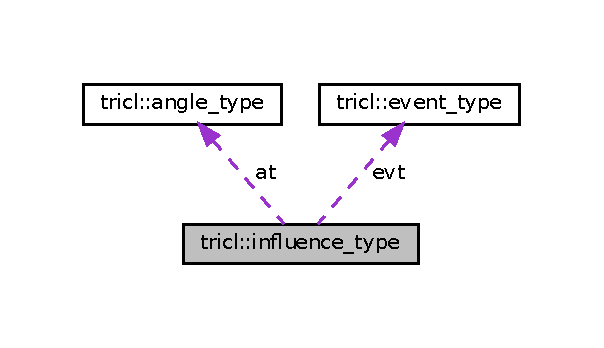
\includegraphics[width=270pt]{d0/dba/structtricl_1_1influence__type__coll__graph}
\end{center}
\end{figure}
\subsection*{Data Fields}
\begin{DoxyCompactItemize}
\item 
\mbox{\Hypertarget{structtricl_1_1influence__type_a9e3a80224b266e0ff8041644e372fe19}\label{structtricl_1_1influence__type_a9e3a80224b266e0ff8041644e372fe19}} 
const \hyperlink{structtricl_1_1event__type}{event\+\_\+type} {\bfseries evt}
\item 
\mbox{\Hypertarget{structtricl_1_1influence__type_a9d6fecd13fbb3e7b0686556d80b3b537}\label{structtricl_1_1influence__type_a9d6fecd13fbb3e7b0686556d80b3b537}} 
const \hyperlink{structtricl_1_1angle__type}{angle\+\_\+type} {\bfseries at}
\end{DoxyCompactItemize}
\subsection*{Friends}
\begin{DoxyCompactItemize}
\item 
\mbox{\Hypertarget{structtricl_1_1influence__type_a4f5b42686b09f580c15f8fa9f3aa296f}\label{structtricl_1_1influence__type_a4f5b42686b09f580c15f8fa9f3aa296f}} 
bool {\bfseries operator==} (const \hyperlink{structtricl_1_1influence__type}{influence\+\_\+type} \&left, const \hyperlink{structtricl_1_1influence__type}{influence\+\_\+type} \&right)
\end{DoxyCompactItemize}


The documentation for this struct was generated from the following file\+:\begin{DoxyCompactItemize}
\item 
src/\hyperlink{data__model_8h}{data\+\_\+model.\+h}\end{DoxyCompactItemize}

\hypertarget{structtricl_1_1inleg}{}\section{tricl\+:\+:inleg Struct Reference}
\label{structtricl_1_1inleg}\index{tricl\+::inleg@{tricl\+::inleg}}


An inleg represents a leg \char`\"{}incoming\char`\"{} to a target entity.  




{\ttfamily \#include $<$data\+\_\+model.\+h$>$}

\subsection*{Data Fields}
\begin{DoxyCompactItemize}
\item 
\mbox{\Hypertarget{structtricl_1_1inleg_a6bdf67f9629e590cebfa4b87d30cf4c6}\label{structtricl_1_1inleg_a6bdf67f9629e590cebfa4b87d30cf4c6}} 
\hyperlink{namespacetricl_a57273122278e8b301844e2a2e1f0742f}{entity} \hyperlink{structtricl_1_1inleg_a6bdf67f9629e590cebfa4b87d30cf4c6}{e\+\_\+source}
\begin{DoxyCompactList}\small\item\em Source entity of the leg. Plays a similar role as {\ttfamily e2} in an angle. \end{DoxyCompactList}\item 
\mbox{\Hypertarget{structtricl_1_1inleg_a5119f9bdfc64539b95279288762b39e3}\label{structtricl_1_1inleg_a5119f9bdfc64539b95279288762b39e3}} 
\hyperlink{namespacetricl_a2d01894944fb58a8fedc0912a48d13f8}{relationship\+\_\+or\+\_\+action\+\_\+type} \hyperlink{structtricl_1_1inleg_a5119f9bdfc64539b95279288762b39e3}{rat\+\_\+in}
\begin{DoxyCompactList}\small\item\em Plays a similar role as {\ttfamily rat23} in an angle. \end{DoxyCompactList}\end{DoxyCompactItemize}
\subsection*{Friends}
\begin{DoxyCompactItemize}
\item 
\mbox{\Hypertarget{structtricl_1_1inleg_a2882c00597e94a9fb19cde857cfe5003}\label{structtricl_1_1inleg_a2882c00597e94a9fb19cde857cfe5003}} 
bool {\bfseries operator==} (const \hyperlink{structtricl_1_1inleg}{inleg} \&left, const \hyperlink{structtricl_1_1inleg}{inleg} \&right)
\item 
\mbox{\Hypertarget{structtricl_1_1inleg_a8ddd31813cdcbb1b7c88d51fcd01cd23}\label{structtricl_1_1inleg_a8ddd31813cdcbb1b7c88d51fcd01cd23}} 
bool {\bfseries operator$<$} (const \hyperlink{structtricl_1_1inleg}{inleg} \&left, const \hyperlink{structtricl_1_1inleg}{inleg} \&right)
\end{DoxyCompactItemize}


\subsection{Detailed Description}
An inleg represents a leg \char`\"{}incoming\char`\"{} to a target entity. 

When an inleg is used, the target entity is clear from the context, hence it is not named itself in the inleg but only the source entity and relationship or action type are stored.

Inlegs may influence the attempt rate or success probability of \char`\"{}adjacent\char`\"{} events (events with the same target entity). 

The documentation for this struct was generated from the following file\+:\begin{DoxyCompactItemize}
\item 
src/\hyperlink{data__model_8h}{data\+\_\+model.\+h}\end{DoxyCompactItemize}

\hypertarget{structtricl_1_1link}{}\section{tricl\+:\+:link Struct Reference}
\label{structtricl_1_1link}\index{tricl\+::link@{tricl\+::link}}


A link encodes either the existence of a certain relationship between two entities (or the cumulative impact of all past actions of a certain type between two entities -- not yet implemented).  




{\ttfamily \#include $<$data\+\_\+model.\+h$>$}

\subsection*{Data Fields}
\begin{DoxyCompactItemize}
\item 
\mbox{\Hypertarget{structtricl_1_1link_a94b71567d0a342c8d0bf28e4fea1dff4}\label{structtricl_1_1link_a94b71567d0a342c8d0bf28e4fea1dff4}} 
const \hyperlink{namespacetricl_a57273122278e8b301844e2a2e1f0742f}{entity} \hyperlink{structtricl_1_1link_a94b71567d0a342c8d0bf28e4fea1dff4}{e1}
\begin{DoxyCompactList}\small\item\em Source entity (or, if $<$0, source entity type of a summary event) \end{DoxyCompactList}\item 
\mbox{\Hypertarget{structtricl_1_1link_a9a21745032378ca68f88966d78814be0}\label{structtricl_1_1link_a9a21745032378ca68f88966d78814be0}} 
const \hyperlink{namespacetricl_a2d01894944fb58a8fedc0912a48d13f8}{relationship\+\_\+or\+\_\+action\+\_\+type} \hyperlink{structtricl_1_1link_a9a21745032378ca68f88966d78814be0}{rat13}
\begin{DoxyCompactList}\small\item\em Type of relationship or action represented by this link. \end{DoxyCompactList}\item 
\mbox{\Hypertarget{structtricl_1_1link_ad54f7dbfcda5fd3f98ff5db897893c87}\label{structtricl_1_1link_ad54f7dbfcda5fd3f98ff5db897893c87}} 
const \hyperlink{namespacetricl_a57273122278e8b301844e2a2e1f0742f}{entity} \hyperlink{structtricl_1_1link_ad54f7dbfcda5fd3f98ff5db897893c87}{e3}
\begin{DoxyCompactList}\small\item\em Target entity (or, if $<$0, target entity type of a summary event) \end{DoxyCompactList}\end{DoxyCompactItemize}
\subsection*{Friends}
\begin{DoxyCompactItemize}
\item 
\mbox{\Hypertarget{structtricl_1_1link_a383e61e15072ef3fe9e16102dea483e0}\label{structtricl_1_1link_a383e61e15072ef3fe9e16102dea483e0}} 
bool {\bfseries operator==} (const \hyperlink{structtricl_1_1link}{link} \&left, const \hyperlink{structtricl_1_1link}{link} \&right)
\item 
\mbox{\Hypertarget{structtricl_1_1link_af79bc13140c8180154526642748b0c33}\label{structtricl_1_1link_af79bc13140c8180154526642748b0c33}} 
bool {\bfseries operator$<$} (const \hyperlink{structtricl_1_1link}{link} \&left, const \hyperlink{structtricl_1_1link}{link} \&right)
\end{DoxyCompactItemize}


\subsection{Detailed Description}
A link encodes either the existence of a certain relationship between two entities (or the cumulative impact of all past actions of a certain type between two entities -- not yet implemented). 

The documentation for this struct was generated from the following file\+:\begin{DoxyCompactItemize}
\item 
src/\hyperlink{data__model_8h}{data\+\_\+model.\+h}\end{DoxyCompactItemize}

\hypertarget{structtricl_1_1link__type}{}\section{tricl\+:\+:link\+\_\+type Struct Reference}
\label{structtricl_1_1link__type}\index{tricl\+::link\+\_\+type@{tricl\+::link\+\_\+type}}


The type of a link is given by two entity types and a relationship or action type.  




{\ttfamily \#include $<$data\+\_\+model.\+h$>$}

\subsection*{Data Fields}
\begin{DoxyCompactItemize}
\item 
\mbox{\Hypertarget{structtricl_1_1link__type_a9cb3cda7790fc4d697f6274cf0af708c}\label{structtricl_1_1link__type_a9cb3cda7790fc4d697f6274cf0af708c}} 
const \hyperlink{namespacetricl_afd4de3aedd5e48cf955f03457386e98f}{entity\+\_\+type} \hyperlink{structtricl_1_1link__type_a9cb3cda7790fc4d697f6274cf0af708c}{et1}
\begin{DoxyCompactList}\small\item\em Type of source entity e1 occurring in this type of link. \end{DoxyCompactList}\item 
\mbox{\Hypertarget{structtricl_1_1link__type_ab567b0eff4a068b28141da69c810770d}\label{structtricl_1_1link__type_ab567b0eff4a068b28141da69c810770d}} 
const \hyperlink{namespacetricl_a2d01894944fb58a8fedc0912a48d13f8}{relationship\+\_\+or\+\_\+action\+\_\+type} \hyperlink{structtricl_1_1link__type_ab567b0eff4a068b28141da69c810770d}{rat13}
\begin{DoxyCompactList}\small\item\em Type of relationship or action represented by this type of link. \end{DoxyCompactList}\item 
\mbox{\Hypertarget{structtricl_1_1link__type_ae89141e8c4719830d32c0d7fe95a184f}\label{structtricl_1_1link__type_ae89141e8c4719830d32c0d7fe95a184f}} 
const \hyperlink{namespacetricl_afd4de3aedd5e48cf955f03457386e98f}{entity\+\_\+type} \hyperlink{structtricl_1_1link__type_ae89141e8c4719830d32c0d7fe95a184f}{et3}
\begin{DoxyCompactList}\small\item\em Type of target entity e3 occurring in this type of link. \end{DoxyCompactList}\end{DoxyCompactItemize}
\subsection*{Friends}
\begin{DoxyCompactItemize}
\item 
\mbox{\Hypertarget{structtricl_1_1link__type_ae75460e218908d70af1163248317096e}\label{structtricl_1_1link__type_ae75460e218908d70af1163248317096e}} 
bool {\bfseries operator==} (const \hyperlink{structtricl_1_1link__type}{link\+\_\+type} \&left, const \hyperlink{structtricl_1_1link__type}{link\+\_\+type} \&right)
\end{DoxyCompactItemize}


\subsection{Detailed Description}
The type of a link is given by two entity types and a relationship or action type. 

The documentation for this struct was generated from the following file\+:\begin{DoxyCompactItemize}
\item 
src/\hyperlink{data__model_8h}{data\+\_\+model.\+h}\end{DoxyCompactItemize}

\hypertarget{structtricl_1_1outleg}{}\section{tricl\+:\+:outleg Struct Reference}
\label{structtricl_1_1outleg}\index{tricl\+::outleg@{tricl\+::outleg}}


An outleg represents a leg \char`\"{}outgoing\char`\"{} from a source entity.  




{\ttfamily \#include $<$data\+\_\+model.\+h$>$}

\subsection*{Data Fields}
\begin{DoxyCompactItemize}
\item 
\mbox{\Hypertarget{structtricl_1_1outleg_a126702ea981b412b0536b34457e92f45}\label{structtricl_1_1outleg_a126702ea981b412b0536b34457e92f45}} 
\hyperlink{namespacetricl_a2d01894944fb58a8fedc0912a48d13f8}{relationship\+\_\+or\+\_\+action\+\_\+type} \hyperlink{structtricl_1_1outleg_a126702ea981b412b0536b34457e92f45}{rat\+\_\+out}
\begin{DoxyCompactList}\small\item\em Plays a similar role as {\ttfamily rat12} in an angle. \end{DoxyCompactList}\item 
\mbox{\Hypertarget{structtricl_1_1outleg_a7329dd10bd2213695049e0b816ab34ce}\label{structtricl_1_1outleg_a7329dd10bd2213695049e0b816ab34ce}} 
\hyperlink{namespacetricl_a57273122278e8b301844e2a2e1f0742f}{entity} \hyperlink{structtricl_1_1outleg_a7329dd10bd2213695049e0b816ab34ce}{e\+\_\+target}
\begin{DoxyCompactList}\small\item\em Target entity of the leg. Plays a similar role as {\ttfamily e2} in an angle. \end{DoxyCompactList}\end{DoxyCompactItemize}
\subsection*{Friends}
\begin{DoxyCompactItemize}
\item 
\mbox{\Hypertarget{structtricl_1_1outleg_a925572d2a4bc56d312134f995f7790a5}\label{structtricl_1_1outleg_a925572d2a4bc56d312134f995f7790a5}} 
bool {\bfseries operator==} (const \hyperlink{structtricl_1_1outleg}{outleg} \&left, const \hyperlink{structtricl_1_1outleg}{outleg} \&right)
\item 
\mbox{\Hypertarget{structtricl_1_1outleg_a594b6be76b1271da95305f64d3f28f52}\label{structtricl_1_1outleg_a594b6be76b1271da95305f64d3f28f52}} 
bool {\bfseries operator$<$} (const \hyperlink{structtricl_1_1outleg}{outleg} \&left, const \hyperlink{structtricl_1_1outleg}{outleg} \&right)
\end{DoxyCompactItemize}


\subsection{Detailed Description}
An outleg represents a leg \char`\"{}outgoing\char`\"{} from a source entity. 

When an outleg is used, the source entity is clear from the context, hence it is not named itself in the outleg but only the target entity and relationship or action type are stored.

Outlegs may influence the attempt rate or success probability of \char`\"{}adjacent\char`\"{} events (events with the same source entity). 

The documentation for this struct was generated from the following file\+:\begin{DoxyCompactItemize}
\item 
src/\hyperlink{data__model_8h}{data\+\_\+model.\+h}\end{DoxyCompactItemize}

\chapter{File Documentation}
\hypertarget{angle_8h}{}\section{src/angle.h File Reference}
\label{angle_8h}\index{src/angle.\+h@{src/angle.\+h}}


Performance-\/critical inline functions for handling of angles.  


{\ttfamily \#include \char`\"{}global\+\_\+variables.\+h\char`\"{}}\newline
{\ttfamily \#include \char`\"{}probability.\+h\char`\"{}}\newline
{\ttfamily \#include \char`\"{}debugging.\+h\char`\"{}}\newline
{\ttfamily \#include \char`\"{}event.\+h\char`\"{}}\newline
{\ttfamily \#include \char`\"{}io.\+h\char`\"{}}\newline
Include dependency graph for angle.\+h\+:\nopagebreak
\begin{figure}[H]
\begin{center}
\leavevmode
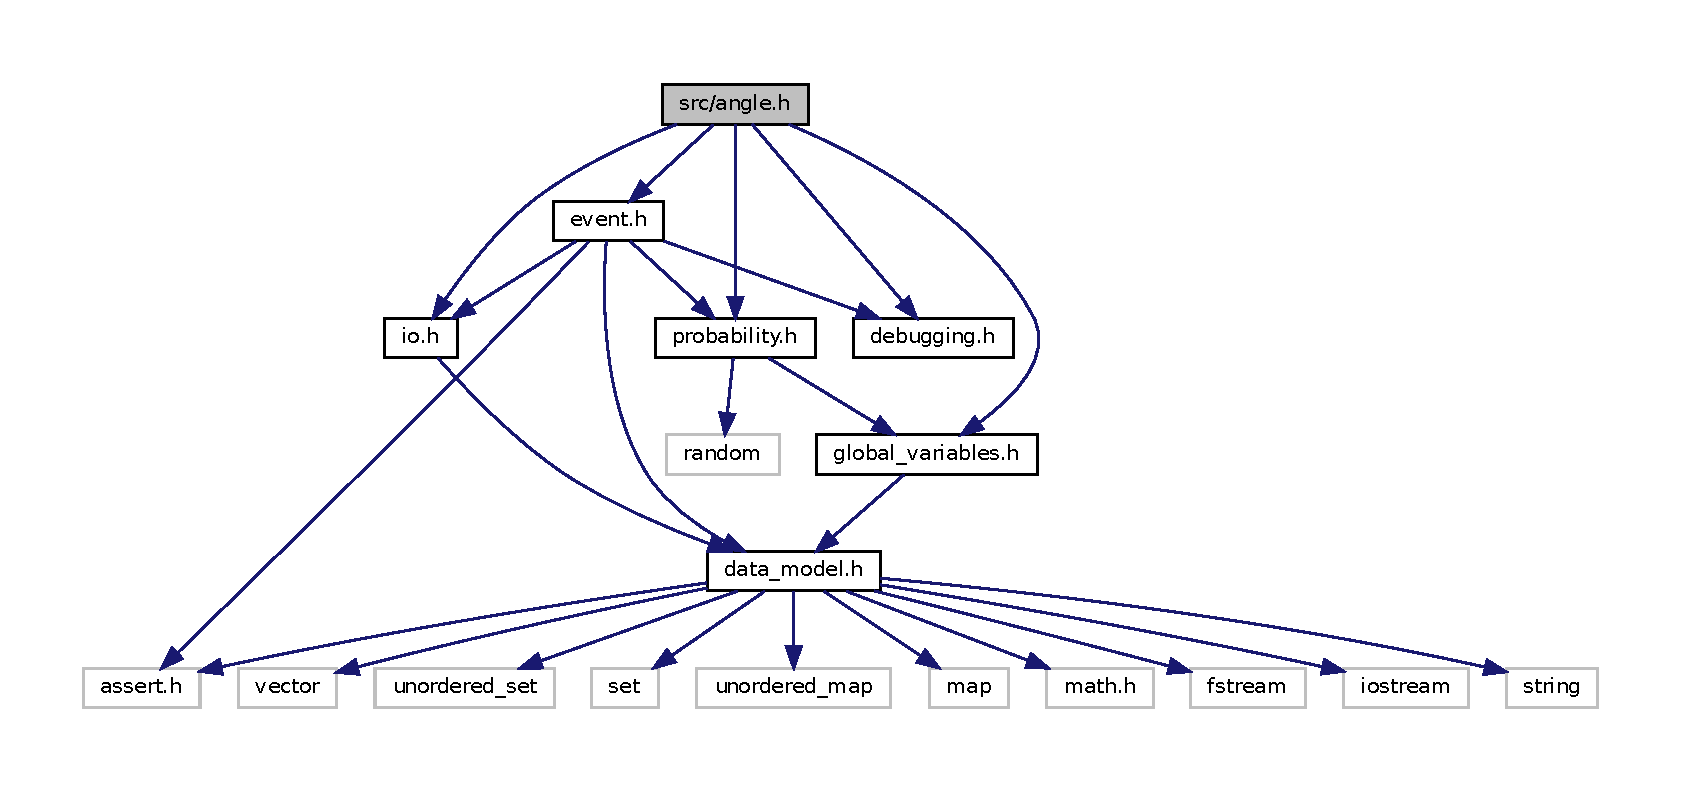
\includegraphics[width=350pt]{da/d9b/angle_8h__incl}
\end{center}
\end{figure}
This graph shows which files directly or indirectly include this file\+:\nopagebreak
\begin{figure}[H]
\begin{center}
\leavevmode
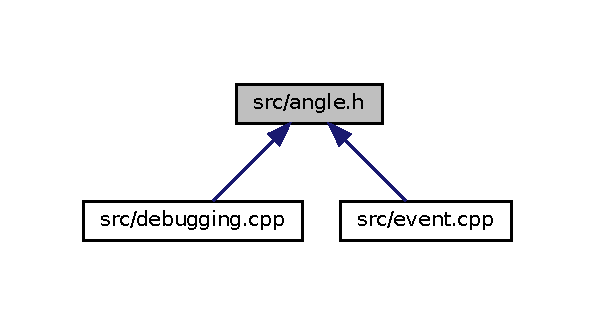
\includegraphics[width=286pt]{d1/d39/angle_8h__dep__incl}
\end{center}
\end{figure}
\subsection*{Functions}
\begin{DoxyCompactItemize}
\item 
void \hyperlink{angle_8h_a1a5dff9417edeae00cf8bfd75459fc36}{add\+\_\+or\+\_\+delete\+\_\+angle} (\hyperlink{namespacetricl_a6967089e2c0837f273d8cb5fd9f7e46d}{event\+\_\+class} ec\+\_\+angle, \hyperlink{namespacetricl_a57273122278e8b301844e2a2e1f0742f}{entity} e1, \hyperlink{namespacetricl_afd4de3aedd5e48cf955f03457386e98f}{entity\+\_\+type} et1, \hyperlink{namespacetricl_a2d01894944fb58a8fedc0912a48d13f8}{relationship\+\_\+or\+\_\+action\+\_\+type} rat12, \hyperlink{namespacetricl_a57273122278e8b301844e2a2e1f0742f}{entity} e2, \hyperlink{namespacetricl_afd4de3aedd5e48cf955f03457386e98f}{entity\+\_\+type} et2, \hyperlink{namespacetricl_a2d01894944fb58a8fedc0912a48d13f8}{relationship\+\_\+or\+\_\+action\+\_\+type} rat23, \hyperlink{namespacetricl_a57273122278e8b301844e2a2e1f0742f}{entity} e3, \hyperlink{namespacetricl_afd4de3aedd5e48cf955f03457386e98f}{entity\+\_\+type} et3)
\begin{DoxyCompactList}\small\item\em Perform all necessary changes in state and event data due to the addition or deletion of an angle. \end{DoxyCompactList}\item 
angle\+\_\+vec \hyperlink{angle_8h_a41fd7245e9c518d475b54f06b741fafb}{leg\+\_\+intersection} (const \hyperlink{namespacetricl_a57273122278e8b301844e2a2e1f0742f}{entity} e1, const \hyperlink{namespacetricl_ab38d0de463e15641fa11e175c60a265e}{outleg\+\_\+set} \&out1, const \hyperlink{namespacetricl_a024e365a54b0a7ed2094f9d452d52a84}{inleg\+\_\+set} \&in3, const \hyperlink{namespacetricl_a57273122278e8b301844e2a2e1f0742f}{entity} e3)
\begin{DoxyCompactList}\small\item\em Compare each outleg of e1 with each inleg of e3 to find each angle from e1 to e3. \end{DoxyCompactList}\end{DoxyCompactItemize}


\subsection{Detailed Description}
Performance-\/critical inline functions for handling of angles. 

See \hyperlink{data__model_8h}{data\+\_\+model.\+h} for how a \hyperlink{structtricl_1_1angle}{tricl\+::angle} relates to other tricl datatypes. 

\subsection{Function Documentation}
\mbox{\Hypertarget{angle_8h_a1a5dff9417edeae00cf8bfd75459fc36}\label{angle_8h_a1a5dff9417edeae00cf8bfd75459fc36}} 
\index{angle.\+h@{angle.\+h}!add\+\_\+or\+\_\+delete\+\_\+angle@{add\+\_\+or\+\_\+delete\+\_\+angle}}
\index{add\+\_\+or\+\_\+delete\+\_\+angle@{add\+\_\+or\+\_\+delete\+\_\+angle}!angle.\+h@{angle.\+h}}
\subsubsection{\texorpdfstring{add\+\_\+or\+\_\+delete\+\_\+angle()}{add\_or\_delete\_angle()}}
{\footnotesize\ttfamily void add\+\_\+or\+\_\+delete\+\_\+angle (\begin{DoxyParamCaption}\item[{\hyperlink{namespacetricl_a6967089e2c0837f273d8cb5fd9f7e46d}{event\+\_\+class}}]{ec\+\_\+angle,  }\item[{\hyperlink{namespacetricl_a57273122278e8b301844e2a2e1f0742f}{entity}}]{e1,  }\item[{\hyperlink{namespacetricl_afd4de3aedd5e48cf955f03457386e98f}{entity\+\_\+type}}]{et1,  }\item[{\hyperlink{namespacetricl_a2d01894944fb58a8fedc0912a48d13f8}{relationship\+\_\+or\+\_\+action\+\_\+type}}]{rat12,  }\item[{\hyperlink{namespacetricl_a57273122278e8b301844e2a2e1f0742f}{entity}}]{e2,  }\item[{\hyperlink{namespacetricl_afd4de3aedd5e48cf955f03457386e98f}{entity\+\_\+type}}]{et2,  }\item[{\hyperlink{namespacetricl_a2d01894944fb58a8fedc0912a48d13f8}{relationship\+\_\+or\+\_\+action\+\_\+type}}]{rat23,  }\item[{\hyperlink{namespacetricl_a57273122278e8b301844e2a2e1f0742f}{entity}}]{e3,  }\item[{\hyperlink{namespacetricl_afd4de3aedd5e48cf955f03457386e98f}{entity\+\_\+type}}]{et3 }\end{DoxyParamCaption})\hspace{0.3cm}{\ttfamily [inline]}}



Perform all necessary changes in state and event data due to the addition or deletion of an angle. 

Iterate through all events that might be influenced by this angle, update their attempt rates and success probability units, and (re)schedule them based on the new rates.

This is one of the performance bottleneck functions since it is called many times by \hyperlink{event_8cpp_adc013b33a8b8afbb4f75c8c95dc3b93a}{update\+\_\+adjacent\+\_\+events()}. 
\begin{DoxyParams}[1]{Parameters}
\mbox{\tt in}  & {\em ec\+\_\+angle} & class of the event that caused the change\+: E\+C\+\_\+\+E\+ST adds an angle, E\+C\+\_\+\+T\+E\+RM deletes one \\
\hline
\mbox{\tt in}  & {\em e1} & source entity \\
\hline
\mbox{\tt in}  & {\em et1} & its type \\
\hline
\mbox{\tt in}  & {\em rat12} & source-\/to-\/middle relationship or action type \\
\hline
\mbox{\tt in}  & {\em e2} & middle entity \\
\hline
\mbox{\tt in}  & {\em et2} & its type \\
\hline
\mbox{\tt in}  & {\em rat23} & middle-\/to-\/target relationship or action type \\
\hline
\mbox{\tt in}  & {\em e3} & target entity \\
\hline
\mbox{\tt in}  & {\em et3} & its type \\
\hline
\end{DoxyParams}
\mbox{\Hypertarget{angle_8h_a41fd7245e9c518d475b54f06b741fafb}\label{angle_8h_a41fd7245e9c518d475b54f06b741fafb}} 
\index{angle.\+h@{angle.\+h}!leg\+\_\+intersection@{leg\+\_\+intersection}}
\index{leg\+\_\+intersection@{leg\+\_\+intersection}!angle.\+h@{angle.\+h}}
\subsubsection{\texorpdfstring{leg\+\_\+intersection()}{leg\_intersection()}}
{\footnotesize\ttfamily angle\+\_\+vec leg\+\_\+intersection (\begin{DoxyParamCaption}\item[{const \hyperlink{namespacetricl_a57273122278e8b301844e2a2e1f0742f}{entity}}]{e1,  }\item[{const \hyperlink{namespacetricl_ab38d0de463e15641fa11e175c60a265e}{outleg\+\_\+set} \&}]{out1,  }\item[{const \hyperlink{namespacetricl_a024e365a54b0a7ed2094f9d452d52a84}{inleg\+\_\+set} \&}]{in3,  }\item[{const \hyperlink{namespacetricl_a57273122278e8b301844e2a2e1f0742f}{entity}}]{e3 }\end{DoxyParamCaption})\hspace{0.3cm}{\ttfamily [inline]}}



Compare each outleg of e1 with each inleg of e3 to find each angle from e1 to e3. 

This is one of the performance bottleneck functions since it is called by \hyperlink{angle_8h_a1a5dff9417edeae00cf8bfd75459fc36}{add\+\_\+or\+\_\+delete\+\_\+angle()}. It uses a large share of the model\textquotesingle{}s C\+PU time.

(code was adapted from adapted from set\+\_\+intersection template)

\begin{DoxyReturn}{Returns}
a vector of found angles 
\end{DoxyReturn}
\subsubsection*{Algorithm\+: }

The two sequences are sorted by e2 (since std\+::set is an ordered datatype and operator$<$ for legs was implemented accordingly). Pseudocode\+: \begin{DoxyVerb}put blockstart = out1.end().
repeat:
  if out1.e2 < in3.e2, advance out1.
  else if out1.e2 > in3.e2:
    advance in3.
    if blockstart != out1.end():
      if in3.e2 == previous in3.e2, rewind out2 to blockstart
      else put blockstart = out1.end().
  else out1.e2 == in3.e2:
    if blockstart == out1.end(), remember out1 position as blockstart
    store found angle
    advance out1
\end{DoxyVerb}

\begin{DoxyParams}[1]{Parameters}
\mbox{\tt in}  & {\em e1} & source entity \\
\hline
\mbox{\tt in}  & {\em out1} & set of outlegs of source entity \\
\hline
\mbox{\tt in}  & {\em in3} & set of inlegs of target entity \\
\hline
\mbox{\tt in}  & {\em e3} & target entity \\
\hline
\end{DoxyParams}

\hypertarget{config_8cpp}{}\section{src/config.cpp File Reference}
\label{config_8cpp}\index{src/config.\+cpp@{src/config.\+cpp}}


Handling of configuration files.  


{\ttfamily \#include $<$limits.\+h$>$}\\*
{\ttfamily \#include $<$math.\+h$>$}\\*
{\ttfamily \#include $<$iostream$>$}\\*
{\ttfamily \#include \char`\"{}yaml-\/cpp/yaml.\+h\char`\"{}}\\*
{\ttfamily \#include \char`\"{}data\+\_\+model.\+h\char`\"{}}\\*
{\ttfamily \#include \char`\"{}global\+\_\+variables.\+h\char`\"{}}\\*
{\ttfamily \#include \char`\"{}entity.\+h\char`\"{}}\\*
{\ttfamily \#include \char`\"{}io.\+h\char`\"{}}\\*
Include dependency graph for config.\+cpp\+:
\nopagebreak
\begin{figure}[H]
\begin{center}
\leavevmode
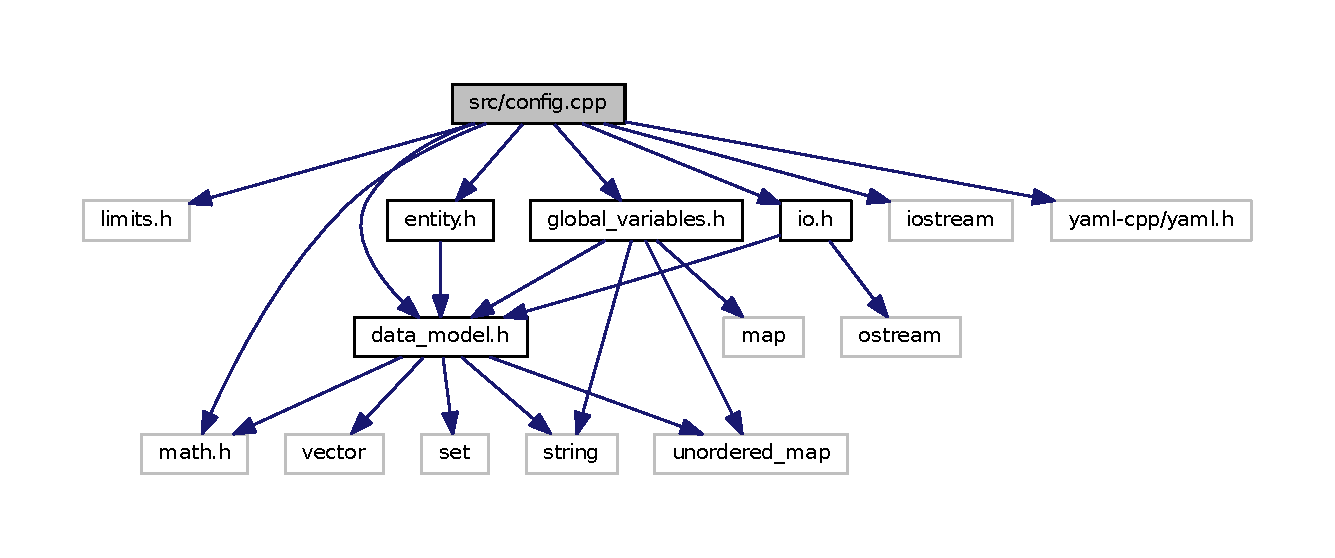
\includegraphics[width=350pt]{db/d4c/config_8cpp__incl}
\end{center}
\end{figure}
\subsection*{Macros}
\begin{DoxyCompactItemize}
\item 
\#define {\bfseries T\+A\+I\+L\+\_\+\+D\+E\+F\+A\+U\+LT}~1.\+0\hypertarget{config_8cpp_a04e254fb2bac4b90010f68d6d716f448}{}\label{config_8cpp_a04e254fb2bac4b90010f68d6d716f448}

\end{DoxyCompactItemize}
\subsection*{Functions}
\begin{DoxyCompactItemize}
\item 
void {\bfseries read\+\_\+entity\+\_\+labels} (Y\+A\+M\+L\+::\+Node n, entity\+\_\+type et)\hypertarget{config_8cpp_ac5594ed0754d45494f17470961e83309}{}\label{config_8cpp_ac5594ed0754d45494f17470961e83309}

\item 
void {\bfseries read\+\_\+config} ()\hypertarget{config_8cpp_ac8471a77a592a1fbe4b3af45fa93098a}{}\label{config_8cpp_ac8471a77a592a1fbe4b3af45fa93098a}

\end{DoxyCompactItemize}
\subsection*{Variables}
\begin{DoxyCompactItemize}
\item 
string {\bfseries gexf\+\_\+filename} = \char`\"{}\char`\"{}\hypertarget{config_8cpp_a0b60e3ce1fbd529d7fb44c1a3b6f2d5a}{}\label{config_8cpp_a0b60e3ce1fbd529d7fb44c1a3b6f2d5a}

\item 
string {\bfseries diagram\+\_\+fileprefix} = \char`\"{}\char`\"{}\hypertarget{config_8cpp_af960657d113135c47b4e0ed4536930c0}{}\label{config_8cpp_af960657d113135c47b4e0ed4536930c0}

\item 
bool {\bfseries verbose} = false\hypertarget{config_8cpp_ab3f078684998b83967d507d0f453f454}{}\label{config_8cpp_ab3f078684998b83967d507d0f453f454}

\item 
bool {\bfseries quiet} = false\hypertarget{config_8cpp_ae4426f467d61ae456b95844d4d9c2dcd}{}\label{config_8cpp_ae4426f467d61ae456b95844d4d9c2dcd}

\item 
bool {\bfseries debug} = false\hypertarget{config_8cpp_a398527b3e9e358c345c5047b16871957}{}\label{config_8cpp_a398527b3e9e358c345c5047b16871957}

\item 
timepoint {\bfseries max\+\_\+t} = I\+N\+F\+I\+N\+I\+TY\hypertarget{config_8cpp_a61e4a08c5309d5cd9538ce9654bdb9e9}{}\label{config_8cpp_a61e4a08c5309d5cd9538ce9654bdb9e9}

\item 
long int {\bfseries max\+\_\+n\+\_\+events} = L\+O\+N\+G\+\_\+\+M\+AX\hypertarget{config_8cpp_a921a3c48e5eda75a9944e3d8fdecc826}{}\label{config_8cpp_a921a3c48e5eda75a9944e3d8fdecc826}

\item 
unsigned {\bfseries seed} = 0\hypertarget{config_8cpp_abb3c5a016eb55b340002c5da33a16714}{}\label{config_8cpp_abb3c5a016eb55b340002c5da33a16714}

\item 
unordered\+\_\+map$<$ entity\+\_\+type, label $>$ {\bfseries et2label} = \{\}\hypertarget{config_8cpp_a1b14b11720f5396f884aba602cc42602}{}\label{config_8cpp_a1b14b11720f5396f884aba602cc42602}

\item 
unordered\+\_\+map$<$ string, entity\+\_\+type $>$ {\bfseries label2et} = \{\}\hypertarget{config_8cpp_a4ad1375a3f0b5760ef4861ef35ac7f25}{}\label{config_8cpp_a4ad1375a3f0b5760ef4861ef35ac7f25}

\item 
unordered\+\_\+map$<$ entity\+\_\+type, entity $>$ {\bfseries et2n} = \{\}\hypertarget{config_8cpp_aba5a0104caf66faf04d0e2f4491415fb}{}\label{config_8cpp_aba5a0104caf66faf04d0e2f4491415fb}

\item 
unordered\+\_\+map$<$ relationship\+\_\+or\+\_\+action\+\_\+type, label $>$ {\bfseries rat2label} = \{ \{R\+T\+\_\+\+ID, \char`\"{}=\char`\"{}\} \}\hypertarget{config_8cpp_a16775be180de048f5d158cf6c18af175}{}\label{config_8cpp_a16775be180de048f5d158cf6c18af175}

\item 
unordered\+\_\+map$<$ string, relationship\+\_\+or\+\_\+action\+\_\+type $>$ {\bfseries label2rat} = \{ \{\char`\"{}=\char`\"{}, R\+T\+\_\+\+ID\} \}\hypertarget{config_8cpp_a1b29491c10222b82a8ac3f8241aa27a8}{}\label{config_8cpp_a1b29491c10222b82a8ac3f8241aa27a8}

\item 
unordered\+\_\+map$<$ relationship\+\_\+or\+\_\+action\+\_\+type, bool $>$ {\bfseries r\+\_\+is\+\_\+action\+\_\+type} = \{\}\hypertarget{config_8cpp_acb03df27c0aec975d0d0a27e21f9b956}{}\label{config_8cpp_acb03df27c0aec975d0d0a27e21f9b956}

\item 
unordered\+\_\+map$<$ relationship\+\_\+or\+\_\+action\+\_\+type, relationship\+\_\+or\+\_\+action\+\_\+type $>$ {\bfseries rat2inv} = \{\}\hypertarget{config_8cpp_a698aaa515390777326d52ab118c9f1fe}{}\label{config_8cpp_a698aaa515390777326d52ab118c9f1fe}

\item 
unordered\+\_\+map$<$ entity, entity\+\_\+type $>$ {\bfseries e2et} = \{\}\hypertarget{config_8cpp_a12b15805ec2a70ba1781f87af3d8215b}{}\label{config_8cpp_a12b15805ec2a70ba1781f87af3d8215b}

\item 
unordered\+\_\+map$<$ entity, label $>$ {\bfseries e2label} = \{\}\hypertarget{config_8cpp_a1d4d2e1edc14bccb896b5dd715cba4a6}{}\label{config_8cpp_a1d4d2e1edc14bccb896b5dd715cba4a6}

\item 
unordered\+\_\+map$<$ string, entity $>$ {\bfseries label2e} = \{\}\hypertarget{config_8cpp_a3e3cf64afa14be51e4752ebe0e78d8b4}{}\label{config_8cpp_a3e3cf64afa14be51e4752ebe0e78d8b4}

\item 
set$<$ \hyperlink{structlink}{link} $>$ {\bfseries initial\+\_\+links} = \{\}\hypertarget{config_8cpp_afe42a9a97fc8e959183c94fc333f2331}{}\label{config_8cpp_afe42a9a97fc8e959183c94fc333f2331}

\item 
unordered\+\_\+map$<$ entity\+\_\+type, int $>$ {\bfseries et2n\+\_\+blocks} = \{\}\hypertarget{config_8cpp_ac3d91d4eef87cfaf1371a698513533ba}{}\label{config_8cpp_ac3d91d4eef87cfaf1371a698513533ba}

\item 
unordered\+\_\+map$<$ \hyperlink{structlink__type}{link\+\_\+type}, probability $>$ {\bfseries lt2initial\+\_\+prob\+\_\+within} = \{\}\hypertarget{config_8cpp_a1cf9b4c5338052d0ac84135ecefc7d39}{}\label{config_8cpp_a1cf9b4c5338052d0ac84135ecefc7d39}

\item 
unordered\+\_\+map$<$ \hyperlink{structlink__type}{link\+\_\+type}, probability $>$ {\bfseries lt2initial\+\_\+prob\+\_\+between} = \{\}\hypertarget{config_8cpp_aa892b7f705910915c42a59b564850a4a}{}\label{config_8cpp_aa892b7f705910915c42a59b564850a4a}

\item 
unordered\+\_\+map$<$ entity\+\_\+type, int $>$ {\bfseries et2dim} = \{\}\hypertarget{config_8cpp_a5022e1a1414fd07a51e1e3e6f08ab064}{}\label{config_8cpp_a5022e1a1414fd07a51e1e3e6f08ab064}

\item 
unordered\+\_\+map$<$ \hyperlink{structlink__type}{link\+\_\+type}, probability $>$ {\bfseries lt2spatial\+\_\+decay} = \{\}\hypertarget{config_8cpp_ac075689bc4d37b273487fa22e5099b32}{}\label{config_8cpp_ac075689bc4d37b273487fa22e5099b32}

\item 
unordered\+\_\+map$<$ \hyperlink{structinfluence__type}{influence\+\_\+type}, rate $>$ {\bfseries inflt2attempt\+\_\+rate} = \{\}\hypertarget{config_8cpp_aa37926f8d74a0c74e47def544c4f872e}{}\label{config_8cpp_aa37926f8d74a0c74e47def544c4f872e}

\item 
unordered\+\_\+map$<$ \hyperlink{structevent__type}{event\+\_\+type}, double $>$ {\bfseries evt2left\+\_\+tail} = \{\}\hypertarget{config_8cpp_ae7b89a8070b4de9d132b167704229c70}{}\label{config_8cpp_ae7b89a8070b4de9d132b167704229c70}

\item 
unordered\+\_\+map$<$ \hyperlink{structevent__type}{event\+\_\+type}, double $>$ {\bfseries evt2right\+\_\+tail} = \{\}\hypertarget{config_8cpp_a6a65e62a5f8173784beb092165af2528}{}\label{config_8cpp_a6a65e62a5f8173784beb092165af2528}

\item 
unordered\+\_\+map$<$ \hyperlink{structevent__type}{event\+\_\+type}, probunits $>$ {\bfseries evt2base\+\_\+probunits} = \{\}\hypertarget{config_8cpp_a5372b5c53ebbceff39a367177d0e4c38}{}\label{config_8cpp_a5372b5c53ebbceff39a367177d0e4c38}

\item 
unordered\+\_\+map$<$ \hyperlink{structinfluence__type}{influence\+\_\+type}, probunits $>$ {\bfseries inflt2delta\+\_\+probunits} = \{\}\hypertarget{config_8cpp_aa4d1d1a030f8a8b177f11e3b4dc93011}{}\label{config_8cpp_aa4d1d1a030f8a8b177f11e3b4dc93011}

\item 
unordered\+\_\+map$<$ entity\+\_\+type, double $>$ {\bfseries et2gexf\+\_\+size} = \{\}\hypertarget{config_8cpp_a922d0c80d1e0778e68aaca86945eb49e}{}\label{config_8cpp_a922d0c80d1e0778e68aaca86945eb49e}

\item 
unordered\+\_\+map$<$ entity\+\_\+type, double $>$ {\bfseries et2gexf\+\_\+a} = \{\}\hypertarget{config_8cpp_a26668024dfdce9d505c1e0ed03a645a2}{}\label{config_8cpp_a26668024dfdce9d505c1e0ed03a645a2}

\item 
unordered\+\_\+map$<$ entity\+\_\+type, string $>$ {\bfseries et2gexf\+\_\+shape} = \{\}\hypertarget{config_8cpp_a10ef80ac6e92253faba86527383b0b19}{}\label{config_8cpp_a10ef80ac6e92253faba86527383b0b19}

\item 
unordered\+\_\+map$<$ entity\+\_\+type, int $>$ {\bfseries et2gexf\+\_\+r} = \{\}\hypertarget{config_8cpp_aa7267315093f6567077ec5e612b46ed1}{}\label{config_8cpp_aa7267315093f6567077ec5e612b46ed1}

\item 
unordered\+\_\+map$<$ entity\+\_\+type, int $>$ {\bfseries et2gexf\+\_\+g} = \{\}\hypertarget{config_8cpp_a86c65c01b4b0c35b56baf6d8d557d977}{}\label{config_8cpp_a86c65c01b4b0c35b56baf6d8d557d977}

\item 
unordered\+\_\+map$<$ entity\+\_\+type, int $>$ {\bfseries et2gexf\+\_\+b} = \{\}\hypertarget{config_8cpp_aded47b9a1ea0cb3ac40ea0ae60d013c3}{}\label{config_8cpp_aded47b9a1ea0cb3ac40ea0ae60d013c3}

\item 
unordered\+\_\+map$<$ relationship\+\_\+or\+\_\+action\+\_\+type, double $>$ {\bfseries rat2gexf\+\_\+thickness} = \{\}\hypertarget{config_8cpp_a7e4baebe848adb451c45c44624784a8a}{}\label{config_8cpp_a7e4baebe848adb451c45c44624784a8a}

\item 
unordered\+\_\+map$<$ relationship\+\_\+or\+\_\+action\+\_\+type, double $>$ {\bfseries rat2gexf\+\_\+a} = \{\}\hypertarget{config_8cpp_a8fc9665235760bdb38eb6a631e654077}{}\label{config_8cpp_a8fc9665235760bdb38eb6a631e654077}

\item 
unordered\+\_\+map$<$ relationship\+\_\+or\+\_\+action\+\_\+type, string $>$ {\bfseries rat2gexf\+\_\+shape} = \{\}\hypertarget{config_8cpp_a9a7b4c97b0337eec7a107d4f48c994f0}{}\label{config_8cpp_a9a7b4c97b0337eec7a107d4f48c994f0}

\item 
unordered\+\_\+map$<$ relationship\+\_\+or\+\_\+action\+\_\+type, int $>$ {\bfseries rat2gexf\+\_\+r} = \{\}\hypertarget{config_8cpp_ad77fa8d20dd7cf1471f2219765253a49}{}\label{config_8cpp_ad77fa8d20dd7cf1471f2219765253a49}

\item 
unordered\+\_\+map$<$ relationship\+\_\+or\+\_\+action\+\_\+type, int $>$ {\bfseries rat2gexf\+\_\+g} = \{\}\hypertarget{config_8cpp_a8063993d6d713ccd233e2fcc6e9bc99b}{}\label{config_8cpp_a8063993d6d713ccd233e2fcc6e9bc99b}

\item 
unordered\+\_\+map$<$ relationship\+\_\+or\+\_\+action\+\_\+type, int $>$ {\bfseries rat2gexf\+\_\+b} = \{\}\hypertarget{config_8cpp_aa91b7e25dfb65b3ea4d7f4c15a7bc25d}{}\label{config_8cpp_aa91b7e25dfb65b3ea4d7f4c15a7bc25d}

\item 
entity {\bfseries max\+\_\+e} = 0\hypertarget{config_8cpp_aca8167edc3c91cb84c829dd88f75c7b4}{}\label{config_8cpp_aca8167edc3c91cb84c829dd88f75c7b4}

\end{DoxyCompactItemize}


\subsection{Detailed Description}
Handling of configuration files. 

Configuration files are in Y\+A\+ML. See config\+\_\+files/parameters\+\_\+\+T\+E\+M\+P\+L\+A\+T\+E.\+yaml for an example

\begin{DoxyAuthor}{Author}
Jobst Heitzig, Potsdam Institute for Climate Impact Research, \href{mailto:heitzig@pik-potsdam.de}{\tt heitzig@pik-\/potsdam.\+de} 
\end{DoxyAuthor}
\begin{DoxyDate}{Date}
Mar 30, 2020 
\end{DoxyDate}

\hypertarget{constants_8cpp}{}\section{src/constants.cpp File Reference}
\label{constants_8cpp}\index{src/constants.\+cpp@{src/constants.\+cpp}}


Some global constants.  


{\ttfamily \#include \char`\"{}data\+\_\+model.\+h\char`\"{}}\newline
Include dependency graph for constants.\+cpp\+:
\nopagebreak
\begin{figure}[H]
\begin{center}
\leavevmode
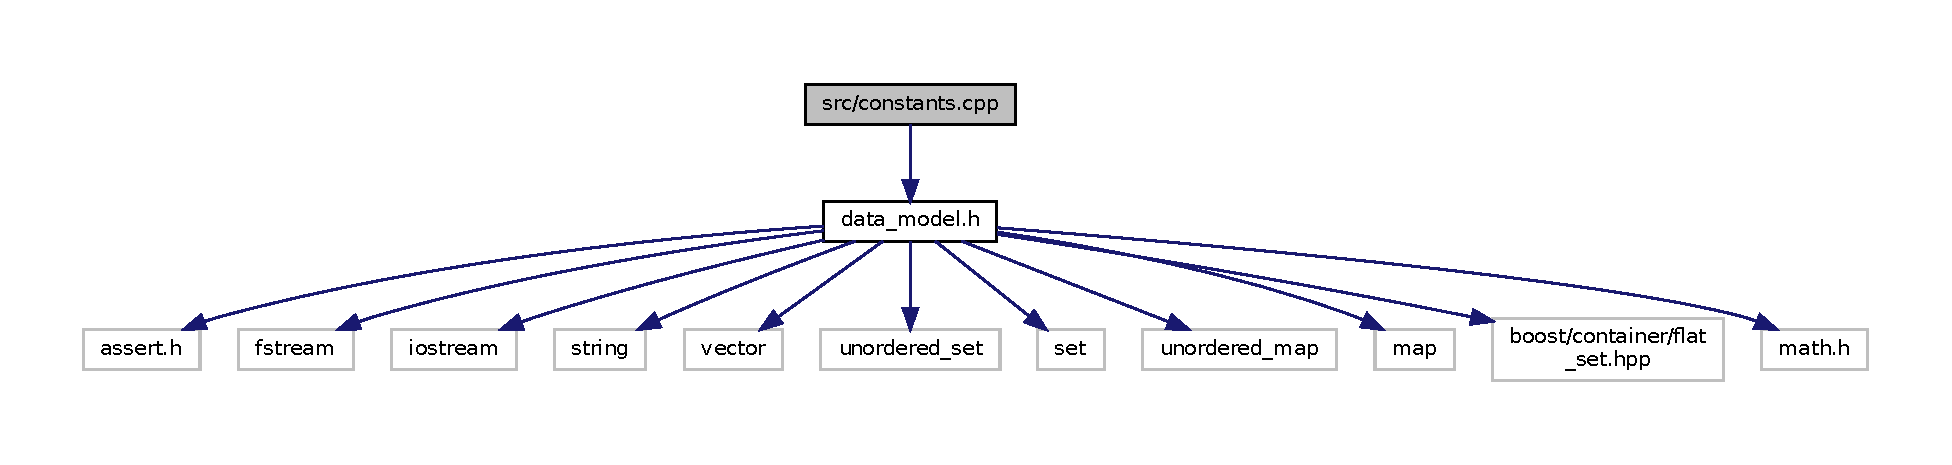
\includegraphics[width=350pt]{d0/d49/constants_8cpp__incl}
\end{center}
\end{figure}
\subsection*{Variables}
\begin{DoxyCompactItemize}
\item 
unordered\+\_\+map$<$ event\+\_\+class, string $>$ {\bfseries tricl\+::ec2label}
\end{DoxyCompactItemize}


\subsection{Detailed Description}
Some global constants. 

\begin{DoxyAuthor}{Author}
Jobst Heitzig, Potsdam Institute for Climate Impact Research, \href{mailto:heitzig@pik-potsdam.de}{\tt heitzig@pik-\/potsdam.\+de} 
\end{DoxyAuthor}
\begin{DoxyDate}{Date}
Mar 30, 2020 
\end{DoxyDate}


\subsection{Variable Documentation}
\mbox{\Hypertarget{constants_8cpp_file_a9f4cb99ed8a0723da68503403d270bf7}\label{constants_8cpp_file_a9f4cb99ed8a0723da68503403d270bf7}} 
\index{constants.\+cpp@{constants.\+cpp}!ec2label@{ec2label}}
\index{ec2label@{ec2label}!constants.\+cpp@{constants.\+cpp}}
\subsubsection{\texorpdfstring{ec2label}{ec2label}}
{\footnotesize\ttfamily unordered\+\_\+map$<$ event\+\_\+class, string $>$ tricl\+::ec2label}

{\bfseries Initial value\+:}
\begin{DoxyCode}
= \{
        \{ EC\_EST, \textcolor{stringliteral}{"establish that"} \},
        \{ EC\_TERM, \textcolor{stringliteral}{"terminate that"} \},
        \{ EC\_ACT, \textcolor{stringliteral}{"let"} \}
    \}
\end{DoxyCode}

\hypertarget{data__model_8h}{}\section{src/data\+\_\+model.h File Reference}
\label{data__model_8h}\index{src/data\+\_\+model.\+h@{src/data\+\_\+model.\+h}}


The main data model.  


{\ttfamily \#include $<$assert.\+h$>$}\newline
{\ttfamily \#include $<$fstream$>$}\newline
{\ttfamily \#include $<$iostream$>$}\newline
{\ttfamily \#include $<$string$>$}\newline
{\ttfamily \#include $<$vector$>$}\newline
{\ttfamily \#include $<$set$>$}\newline
{\ttfamily \#include $<$unordered\+\_\+map$>$}\newline
{\ttfamily \#include $<$map$>$}\newline
{\ttfamily \#include $<$math.\+h$>$}\newline
Include dependency graph for data\+\_\+model.\+h\+:\nopagebreak
\begin{figure}[H]
\begin{center}
\leavevmode
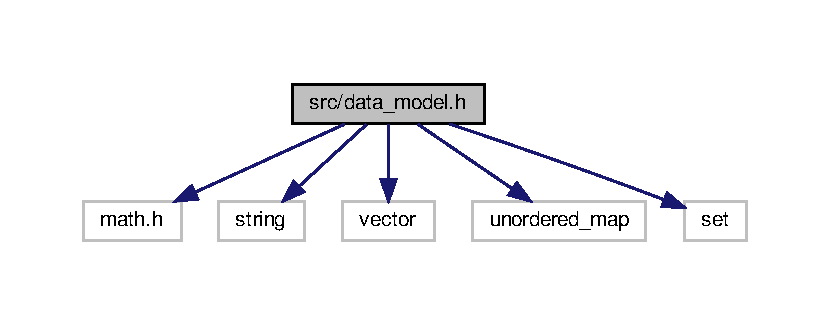
\includegraphics[width=350pt]{d0/dc6/data__model_8h__incl}
\end{center}
\end{figure}
This graph shows which files directly or indirectly include this file\+:\nopagebreak
\begin{figure}[H]
\begin{center}
\leavevmode
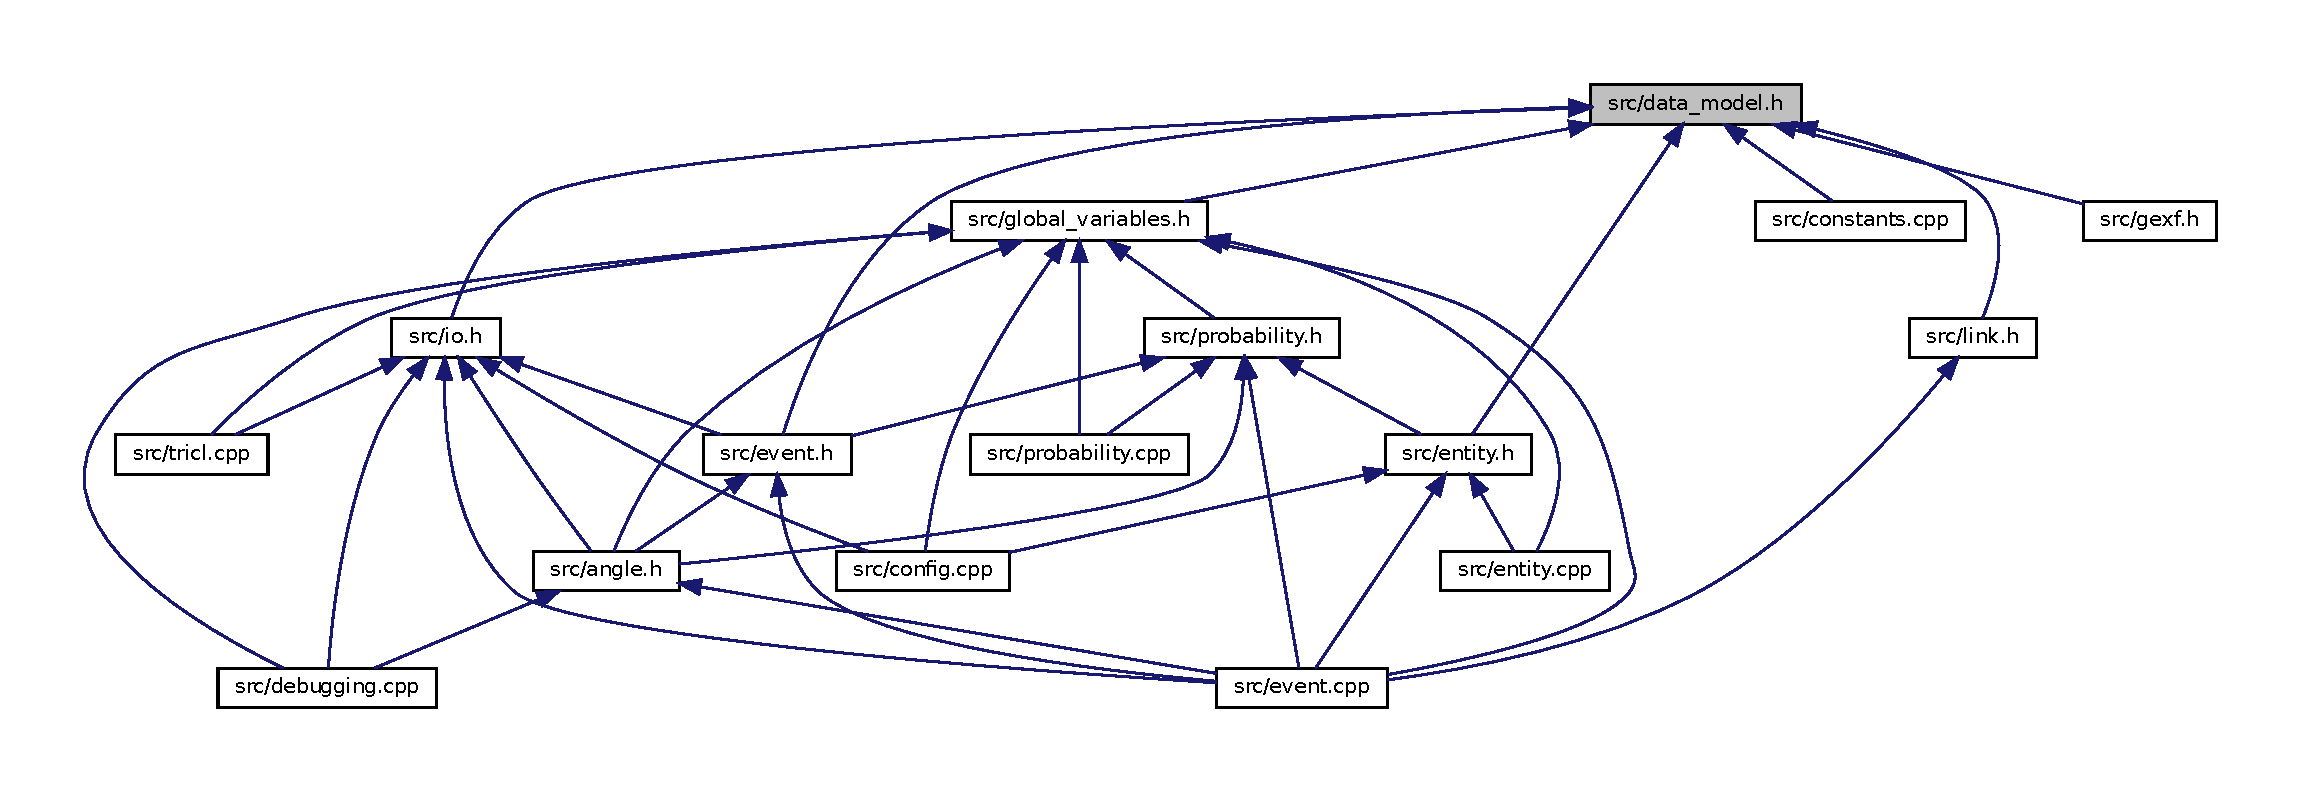
\includegraphics[width=350pt]{d8/d95/data__model_8h__dep__incl}
\end{center}
\end{figure}
\subsection*{Data Structures}
\begin{DoxyCompactItemize}
\item 
struct \hyperlink{structtricl_1_1entity__type__pair}{tricl\+::entity\+\_\+type\+\_\+pair}
\item 
struct \hyperlink{structtricl_1_1link__type}{tricl\+::link\+\_\+type}
\item 
struct \hyperlink{structtricl_1_1event__type}{tricl\+::event\+\_\+type}
\item 
struct \hyperlink{structtricl_1_1angle__type}{tricl\+::angle\+\_\+type}
\item 
struct \hyperlink{structtricl_1_1influence__type}{tricl\+::influence\+\_\+type}
\item 
struct \hyperlink{structtricl_1_1inleg}{tricl\+::inleg}
\item 
struct \hyperlink{structtricl_1_1outleg}{tricl\+::outleg}
\item 
struct \hyperlink{structtricl_1_1link}{tricl\+::link}
\item 
struct \hyperlink{structtricl_1_1event}{tricl\+::event}
\item 
struct \hyperlink{structtricl_1_1event__data}{tricl\+::event\+\_\+data}
\item 
struct \hyperlink{structtricl_1_1angle}{tricl\+::angle}
\item 
struct \hyperlink{structstd_1_1hash_3_01entity__type__pair_01_4}{std\+::hash$<$ entity\+\_\+type\+\_\+pair $>$}
\item 
struct \hyperlink{structstd_1_1hash_3_01link__type_01_4}{std\+::hash$<$ link\+\_\+type $>$}
\item 
struct \hyperlink{structstd_1_1hash_3_01event__type_01_4}{std\+::hash$<$ event\+\_\+type $>$}
\item 
struct \hyperlink{structstd_1_1hash_3_01angle__type_01_4}{std\+::hash$<$ angle\+\_\+type $>$}
\item 
struct \hyperlink{structstd_1_1hash_3_01influence__type_01_4}{std\+::hash$<$ influence\+\_\+type $>$}
\item 
struct \hyperlink{structstd_1_1hash_3_01inleg_01_4}{std\+::hash$<$ inleg $>$}
\item 
struct \hyperlink{structstd_1_1hash_3_01outleg_01_4}{std\+::hash$<$ outleg $>$}
\item 
struct \hyperlink{structstd_1_1hash_3_01link_01_4}{std\+::hash$<$ link $>$}
\item 
struct \hyperlink{structstd_1_1hash_3_01event_01_4}{std\+::hash$<$ event $>$}
\item 
struct \hyperlink{structstd_1_1hash_3_01angle_01_4}{std\+::hash$<$ angle $>$}
\end{DoxyCompactItemize}
\subsection*{Macros}
\begin{DoxyCompactItemize}
\item 
\mbox{\Hypertarget{data__model_8h_a4ef43416c3082b95dfc7b9b4b37ed4a7}\label{data__model_8h_a4ef43416c3082b95dfc7b9b4b37ed4a7}} 
\#define \hyperlink{data__model_8h_a4ef43416c3082b95dfc7b9b4b37ed4a7}{E\+\_\+\+B\+I\+TS}~20
\begin{DoxyCompactList}\small\item\em no. of bits used for entity ids --$>$ max. 1 mio. entities \end{DoxyCompactList}\item 
\mbox{\Hypertarget{data__model_8h_a27e24a1c84c197041afdad0fc49dcaeb}\label{data__model_8h_a27e24a1c84c197041afdad0fc49dcaeb}} 
\#define \hyperlink{data__model_8h_a27e24a1c84c197041afdad0fc49dcaeb}{E\+T\+\_\+\+B\+I\+TS}~4
\begin{DoxyCompactList}\small\item\em no. of bits used for entity types --$>$ max. 16 entity types \end{DoxyCompactList}\item 
\mbox{\Hypertarget{data__model_8h_a1712faaa1ef9bb3dcbfae56161881708}\label{data__model_8h_a1712faaa1ef9bb3dcbfae56161881708}} 
\#define \hyperlink{data__model_8h_a1712faaa1ef9bb3dcbfae56161881708}{R\+A\+T\+\_\+\+B\+I\+TS}~4
\begin{DoxyCompactList}\small\item\em no. of bits used for relationship or action types --$>$ max. 16 relationship or action types \end{DoxyCompactList}\item 
\mbox{\Hypertarget{data__model_8h_acaa7fd772f80b3066211e5eb6e29ed91}\label{data__model_8h_acaa7fd772f80b3066211e5eb6e29ed91}} 
\#define \hyperlink{data__model_8h_acaa7fd772f80b3066211e5eb6e29ed91}{M\+A\+X\+\_\+\+N\+\_\+E}~((1$<$$<$\hyperlink{data__model_8h_a4ef43416c3082b95dfc7b9b4b37ed4a7}{E\+\_\+\+B\+I\+TS})-\/1)
\begin{DoxyCompactList}\small\item\em resulting max. no. of entities \end{DoxyCompactList}\item 
\mbox{\Hypertarget{data__model_8h_ae71ff63a5bdb6bfc09a18840c8df4e54}\label{data__model_8h_ae71ff63a5bdb6bfc09a18840c8df4e54}} 
\#define \hyperlink{data__model_8h_ae71ff63a5bdb6bfc09a18840c8df4e54}{N\+O\+\_\+\+R\+AT}~0
\begin{DoxyCompactList}\small\item\em missing value for relationship or action type, used in angles to encode legs \end{DoxyCompactList}\item 
\mbox{\Hypertarget{data__model_8h_a549fa469b9ccb6e0fe046f797bc181e0}\label{data__model_8h_a549fa469b9ccb6e0fe046f797bc181e0}} 
\#define \hyperlink{data__model_8h_a549fa469b9ccb6e0fe046f797bc181e0}{R\+T\+\_\+\+ID}~1
\begin{DoxyCompactList}\small\item\em relationship type for identity relationship \char`\"{}=\char`\"{}, always present \end{DoxyCompactList}\item 
\mbox{\Hypertarget{data__model_8h_a9a89b5cd637aedee7c32dc74252da764}\label{data__model_8h_a9a89b5cd637aedee7c32dc74252da764}} 
\#define {\bfseries I\+N\+F\+LT}(inflt)~((size\+\_\+t)inflt.\+evt.\+ec $^\wedge$ ((size\+\_\+t)inflt.\+evt.\+et1 $<$$<$ 2) $^\wedge$ ((size\+\_\+t)inflt.\+evt.\+rat13 $<$$<$ (2+\hyperlink{data__model_8h_a27e24a1c84c197041afdad0fc49dcaeb}{E\+T\+\_\+\+B\+I\+TS})) $^\wedge$ ((size\+\_\+t)inflt.\+evt.\+et3 $<$$<$ (2+\hyperlink{data__model_8h_a27e24a1c84c197041afdad0fc49dcaeb}{E\+T\+\_\+\+B\+I\+TS}+\hyperlink{data__model_8h_a1712faaa1ef9bb3dcbfae56161881708}{R\+A\+T\+\_\+\+B\+I\+TS})) $^\wedge$ ((size\+\_\+t)inflt.\+at.\+rat12 $<$$<$ (2+2$\ast$\hyperlink{data__model_8h_a27e24a1c84c197041afdad0fc49dcaeb}{E\+T\+\_\+\+B\+I\+TS}+\hyperlink{data__model_8h_a1712faaa1ef9bb3dcbfae56161881708}{R\+A\+T\+\_\+\+B\+I\+TS})) $^\wedge$ ((size\+\_\+t)inflt.\+at.\+et2 $<$$<$ (2+2$\ast$\hyperlink{data__model_8h_a27e24a1c84c197041afdad0fc49dcaeb}{E\+T\+\_\+\+B\+I\+TS}+2$\ast$\hyperlink{data__model_8h_a1712faaa1ef9bb3dcbfae56161881708}{R\+A\+T\+\_\+\+B\+I\+TS})) $^\wedge$ ((size\+\_\+t)inflt.\+at.\+rat23 $<$$<$ (2+3$\ast$\hyperlink{data__model_8h_a27e24a1c84c197041afdad0fc49dcaeb}{E\+T\+\_\+\+B\+I\+TS}+2$\ast$\hyperlink{data__model_8h_a1712faaa1ef9bb3dcbfae56161881708}{R\+A\+T\+\_\+\+B\+I\+TS})))
\item 
\mbox{\Hypertarget{data__model_8h_a3890372a566c5b111dd6fabda11e73bc}\label{data__model_8h_a3890372a566c5b111dd6fabda11e73bc}} 
\#define {\bfseries M\+A\+X\+\_\+\+N\+\_\+\+I\+N\+F\+LT}~(1 $<$$<$ (2+3$\ast$\hyperlink{data__model_8h_a27e24a1c84c197041afdad0fc49dcaeb}{E\+T\+\_\+\+B\+I\+TS}+3$\ast$\hyperlink{data__model_8h_a1712faaa1ef9bb3dcbfae56161881708}{R\+A\+T\+\_\+\+B\+I\+TS}))
\end{DoxyCompactItemize}
\subsection*{Typedefs}
\begin{DoxyCompactItemize}
\item 
\mbox{\Hypertarget{data__model_8h_a720ff6a29f998e11e1d3622fc8df64b1}\label{data__model_8h_a720ff6a29f998e11e1d3622fc8df64b1}} 
typedef double \hyperlink{data__model_8h_a720ff6a29f998e11e1d3622fc8df64b1}{tricl\+::timepoint}
\begin{DoxyCompactList}\small\item\em a point in continuous model time, 0...inf \end{DoxyCompactList}\item 
\mbox{\Hypertarget{data__model_8h_af8f8f9076e92e1c664ffa96f18d038a5}\label{data__model_8h_af8f8f9076e92e1c664ffa96f18d038a5}} 
typedef double \hyperlink{data__model_8h_af8f8f9076e92e1c664ffa96f18d038a5}{tricl\+::probunits}
\begin{DoxyCompactList}\small\item\em -\/inf...inf, will be mapped to probabilities by means of the function probunits2probability() \end{DoxyCompactList}\item 
\mbox{\Hypertarget{data__model_8h_af2e8973ba58a3dad9061296d8bee16a2}\label{data__model_8h_af2e8973ba58a3dad9061296d8bee16a2}} 
typedef double \hyperlink{data__model_8h_af2e8973ba58a3dad9061296d8bee16a2}{tricl\+::probability}
\begin{DoxyCompactList}\small\item\em 0...1 \end{DoxyCompactList}\item 
\mbox{\Hypertarget{data__model_8h_ae42d2696f294300a43e0f5edf4875479}\label{data__model_8h_ae42d2696f294300a43e0f5edf4875479}} 
typedef double \hyperlink{data__model_8h_ae42d2696f294300a43e0f5edf4875479}{tricl\+::rate}
\begin{DoxyCompactList}\small\item\em probability per time, 0...inf. (inf is used for things happening \char`\"{}immediately\char`\"{}) \end{DoxyCompactList}\item 
\mbox{\Hypertarget{data__model_8h_a77e7daffafa870e5786b344119da9b15}\label{data__model_8h_a77e7daffafa870e5786b344119da9b15}} 
typedef string \hyperlink{data__model_8h_a77e7daffafa870e5786b344119da9b15}{tricl\+::label}
\begin{DoxyCompactList}\small\item\em labels of things \end{DoxyCompactList}\item 
typedef int \hyperlink{data__model_8h_a57273122278e8b301844e2a2e1f0742f}{tricl\+::entity}
\begin{DoxyCompactList}\small\item\em Entities are used to encode all physical and abstract objects of the modeled social dynamics that can stand in some form of relation to another or can perform some kinds of actions on or with another. \end{DoxyCompactList}\item 
typedef short unsigned int \hyperlink{data__model_8h_afd4de3aedd5e48cf955f03457386e98f}{tricl\+::entity\+\_\+type}
\begin{DoxyCompactList}\small\item\em Entity types are used to encode the different kinds of entities in a model. \end{DoxyCompactList}\item 
typedef size\+\_\+t \hyperlink{data__model_8h_a2d01894944fb58a8fedc0912a48d13f8}{tricl\+::relationship\+\_\+or\+\_\+action\+\_\+type}
\begin{DoxyCompactList}\small\item\em Relationship types are used to encode the kinds of relationships entities may stand in; action types are used to encode the kinds of actions entities may perform on or with another (not implemented yet); they are encoded in a common datatype and distinguished by means of the map rat\+\_\+is\+\_\+action\+\_\+type (not implemented yet). \end{DoxyCompactList}\item 
\mbox{\Hypertarget{data__model_8h_a703ed53fa2dba74d8f51ede5fd46038d}\label{data__model_8h_a703ed53fa2dba74d8f51ede5fd46038d}} 
typedef set$<$ \hyperlink{structtricl_1_1inleg}{inleg} $>$ {\bfseries tricl\+::inleg\+\_\+set}
\item 
\mbox{\Hypertarget{data__model_8h_ac36fc4606da3d7f9ffd1764942fe5940}\label{data__model_8h_ac36fc4606da3d7f9ffd1764942fe5940}} 
typedef set$<$ \hyperlink{structtricl_1_1outleg}{outleg} $>$ {\bfseries tricl\+::outleg\+\_\+set}
\item 
\mbox{\Hypertarget{data__model_8h_a4ec9b46d6dae5a1d114387bca4029ce5}\label{data__model_8h_a4ec9b46d6dae5a1d114387bca4029ce5}} 
typedef vector$<$ \hyperlink{structtricl_1_1angle}{angle} $>$ {\bfseries tricl\+::angles}
\end{DoxyCompactItemize}
\subsection*{Enumerations}
\begin{DoxyCompactItemize}
\item 
enum \hyperlink{data__model_8h_a6967089e2c0837f273d8cb5fd9f7e46d}{tricl\+::event\+\_\+class} \{ \hyperlink{data__model_8h_a6967089e2c0837f273d8cb5fd9f7e46da928305067790de15396de8fcc92b72b9}{tricl\+::\+E\+C\+\_\+\+E\+ST}, 
\hyperlink{data__model_8h_a6967089e2c0837f273d8cb5fd9f7e46da16f53be37a75a1cdfc726014c7f3810a}{tricl\+::\+E\+C\+\_\+\+T\+E\+RM}, 
\hyperlink{data__model_8h_a6967089e2c0837f273d8cb5fd9f7e46dac508c68c92ee059322cb644dd330bbcf}{tricl\+::\+E\+C\+\_\+\+A\+CT}
 \}\begin{DoxyCompactList}\small\item\em (don\textquotesingle{}t confuse with event\+\_\+type!) \end{DoxyCompactList}
\end{DoxyCompactItemize}
\subsection*{Variables}
\begin{DoxyCompactItemize}
\item 
\mbox{\Hypertarget{data__model_8h_a1d25690adbc3921709bd3b3e16415713}\label{data__model_8h_a1d25690adbc3921709bd3b3e16415713}} 
const \hyperlink{structtricl_1_1angle__type}{angle\+\_\+type} {\bfseries tricl\+::\+N\+O\+\_\+\+A\+N\+G\+LE} = \{ .rat12 = \hyperlink{data__model_8h_ae71ff63a5bdb6bfc09a18840c8df4e54}{N\+O\+\_\+\+R\+AT}, .et2 = 0, .rat23 = \hyperlink{data__model_8h_ae71ff63a5bdb6bfc09a18840c8df4e54}{N\+O\+\_\+\+R\+AT} \}
\end{DoxyCompactItemize}


\subsection{Detailed Description}
The main data model. 

Defines all structs and their operators.

\begin{DoxyAuthor}{Author}
Jobst Heitzig, Potsdam Institute for Climate Impact Research, \href{mailto:heitzig@pik-potsdam.de}{\tt heitzig@pik-\/potsdam.\+de} 
\end{DoxyAuthor}
\begin{DoxyDate}{Date}
Mar 30, 2020
\end{DoxyDate}
\subsubsection*{Data architecture }

Most data is kept in unordered maps (what would be dictionaries in python) whose keys are entity types, entities, link types, links, legs, angles, event types, events, influence types and influences. the latter types of things are encoded as structs, most of which are basically tuples of integer ids.

For fast access to map entries, these are automatically turned into integer hashs via the hash structs at the end of this file.

Some data (which is accessed most often) is instead kept in vectors whose indices are either entities (which are ints) or integer hash values of influence types (constructed via the macro I\+N\+F\+LT).

All hashs are constructed as logical O\+Rs of properly shifted ids, hence valid ids are restricted by the respective numbers of bits reserved for this id in the hash.

This hash construction is governed by the bit size macros \hyperlink{data__model_8h_a4ef43416c3082b95dfc7b9b4b37ed4a7}{E\+\_\+\+B\+I\+TS}, \hyperlink{data__model_8h_a27e24a1c84c197041afdad0fc49dcaeb}{E\+T\+\_\+\+B\+I\+TS}, and \hyperlink{data__model_8h_a1712faaa1ef9bb3dcbfae56161881708}{R\+A\+T\+\_\+\+B\+I\+TS}, which could be adapted in dependence on system architecture, but must fulfil the following constraints\+: 2 + 2$\ast$\+E\+\_\+\+B\+I\+TS + R\+A\+T\+\_\+\+B\+I\+TS $<$= no. of bits in size\+\_\+t (32 or 64) 2$^\wedge$\+E\+\_\+\+B\+I\+TS + 2$^\wedge$(6 + 3$\ast$\+R\+A\+T\+\_\+\+B\+I\+TS + 3$\ast$\+E\+T\+\_\+\+B\+I\+TS) $<$= available memory bytes 

\subsection{Typedef Documentation}
\mbox{\Hypertarget{data__model_8h_file_a57273122278e8b301844e2a2e1f0742f}\label{data__model_8h_file_a57273122278e8b301844e2a2e1f0742f}} 
\index{data\+\_\+model.\+h@{data\+\_\+model.\+h}!entity@{entity}}
\index{entity@{entity}!data\+\_\+model.\+h@{data\+\_\+model.\+h}}
\subsubsection{\texorpdfstring{entity}{entity}}
{\footnotesize\ttfamily typedef int \hyperlink{data__model_8h_a57273122278e8b301844e2a2e1f0742f}{tricl\+::entity}}



Entities are used to encode all physical and abstract objects of the modeled social dynamics that can stand in some form of relation to another or can perform some kinds of actions on or with another. 

Actual entities have ids $>$= 1. In summary events, the datatype \char`\"{}entity\char`\"{} is also used to store entity types as negative numbers. \mbox{\Hypertarget{data__model_8h_file_afd4de3aedd5e48cf955f03457386e98f}\label{data__model_8h_file_afd4de3aedd5e48cf955f03457386e98f}} 
\index{data\+\_\+model.\+h@{data\+\_\+model.\+h}!entity\+\_\+type@{entity\+\_\+type}}
\index{entity\+\_\+type@{entity\+\_\+type}!data\+\_\+model.\+h@{data\+\_\+model.\+h}}
\subsubsection{\texorpdfstring{entity\+\_\+type}{entity\_type}}
{\footnotesize\ttfamily typedef short unsigned int \hyperlink{data__model_8h_afd4de3aedd5e48cf955f03457386e98f}{tricl\+::entity\+\_\+type}}



Entity types are used to encode the different kinds of entities in a model. 

Examples of entity type labels\+: \char`\"{}user\char`\"{}, \char`\"{}message\char`\"{}, \char`\"{}opinion\char`\"{}, \char`\"{}epidemic status\char`\"{}, \char`\"{}religious group\char`\"{}, \char`\"{}household\char`\"{}, \char`\"{}news channel\char`\"{}$>$=1 so that -\/entity\+\_\+type can be stored in entity fields \mbox{\Hypertarget{data__model_8h_file_a2d01894944fb58a8fedc0912a48d13f8}\label{data__model_8h_file_a2d01894944fb58a8fedc0912a48d13f8}} 
\index{data\+\_\+model.\+h@{data\+\_\+model.\+h}!relationship\+\_\+or\+\_\+action\+\_\+type@{relationship\+\_\+or\+\_\+action\+\_\+type}}
\index{relationship\+\_\+or\+\_\+action\+\_\+type@{relationship\+\_\+or\+\_\+action\+\_\+type}!data\+\_\+model.\+h@{data\+\_\+model.\+h}}
\subsubsection{\texorpdfstring{relationship\+\_\+or\+\_\+action\+\_\+type}{relationship\_or\_action\_type}}
{\footnotesize\ttfamily typedef size\+\_\+t \hyperlink{data__model_8h_a2d01894944fb58a8fedc0912a48d13f8}{tricl\+::relationship\+\_\+or\+\_\+action\+\_\+type}}



Relationship types are used to encode the kinds of relationships entities may stand in; action types are used to encode the kinds of actions entities may perform on or with another (not implemented yet); they are encoded in a common datatype and distinguished by means of the map rat\+\_\+is\+\_\+action\+\_\+type (not implemented yet). 

Both can either be symmetric (undirected) or nonsymmetric (directed).

Examples of labels for symmetric relationship types\+: \char`\"{}is friends with\char`\"{}, \char`\"{}is inconsistent with\char`\"{}, \char`\"{}is a neighbour of\char`\"{}.

Examples of labels for nonsymmetric relationship types\+: \char`\"{}follows\char`\"{}, \char`\"{}has read\char`\"{}, \char`\"{}is in status\char`\"{}, \char`\"{}belongs to\char`\"{}.

Examples of labels for symmetric action types\+: \char`\"{}meets\char`\"{}, \char`\"{}talks to\char`\"{}.

Examples of labels for nonsymmetric action types\+: \char`\"{}broadcasts\char`\"{}, \char`\"{}reads\char`\"{}.$>$= 1 

\subsection{Enumeration Type Documentation}
\mbox{\Hypertarget{data__model_8h_file_a6967089e2c0837f273d8cb5fd9f7e46d}\label{data__model_8h_file_a6967089e2c0837f273d8cb5fd9f7e46d}} 
\index{data\+\_\+model.\+h@{data\+\_\+model.\+h}!event\+\_\+class@{event\+\_\+class}}
\index{event\+\_\+class@{event\+\_\+class}!data\+\_\+model.\+h@{data\+\_\+model.\+h}}
\subsubsection{\texorpdfstring{event\+\_\+class}{event\_class}}
{\footnotesize\ttfamily enum \hyperlink{data__model_8h_a6967089e2c0837f273d8cb5fd9f7e46d}{tricl\+::event\+\_\+class}}



(don\textquotesingle{}t confuse with event\+\_\+type!) 

\begin{DoxyEnumFields}{Enumerator}
\raisebox{\heightof{T}}[0pt][0pt]{\index{E\+C\+\_\+\+E\+ST@{E\+C\+\_\+\+E\+ST}!data\+\_\+model.\+h@{data\+\_\+model.\+h}}\index{data\+\_\+model.\+h@{data\+\_\+model.\+h}!E\+C\+\_\+\+E\+ST@{E\+C\+\_\+\+E\+ST}}}\mbox{\Hypertarget{data__model_8h_a6967089e2c0837f273d8cb5fd9f7e46da928305067790de15396de8fcc92b72b9}\label{data__model_8h_a6967089e2c0837f273d8cb5fd9f7e46da928305067790de15396de8fcc92b72b9}} 
E\+C\+\_\+\+E\+ST&establishment of a relationship \\
\hline

\raisebox{\heightof{T}}[0pt][0pt]{\index{E\+C\+\_\+\+T\+E\+RM@{E\+C\+\_\+\+T\+E\+RM}!data\+\_\+model.\+h@{data\+\_\+model.\+h}}\index{data\+\_\+model.\+h@{data\+\_\+model.\+h}!E\+C\+\_\+\+T\+E\+RM@{E\+C\+\_\+\+T\+E\+RM}}}\mbox{\Hypertarget{data__model_8h_a6967089e2c0837f273d8cb5fd9f7e46da16f53be37a75a1cdfc726014c7f3810a}\label{data__model_8h_a6967089e2c0837f273d8cb5fd9f7e46da16f53be37a75a1cdfc726014c7f3810a}} 
E\+C\+\_\+\+T\+E\+RM&termination of a relationship \\
\hline

\raisebox{\heightof{T}}[0pt][0pt]{\index{E\+C\+\_\+\+A\+CT@{E\+C\+\_\+\+A\+CT}!data\+\_\+model.\+h@{data\+\_\+model.\+h}}\index{data\+\_\+model.\+h@{data\+\_\+model.\+h}!E\+C\+\_\+\+A\+CT@{E\+C\+\_\+\+A\+CT}}}\mbox{\Hypertarget{data__model_8h_a6967089e2c0837f273d8cb5fd9f7e46dac508c68c92ee059322cb644dd330bbcf}\label{data__model_8h_a6967089e2c0837f273d8cb5fd9f7e46dac508c68c92ee059322cb644dd330bbcf}} 
E\+C\+\_\+\+A\+CT&occurrence of an action \\
\hline

\end{DoxyEnumFields}

\hypertarget{debugging_8cpp}{}\section{src/debugging.cpp File Reference}
\label{debugging_8cpp}\index{src/debugging.\+cpp@{src/debugging.\+cpp}}


Some stuff only needed for debugging.  


{\ttfamily \#include \char`\"{}assert.\+h\char`\"{}}\newline
{\ttfamily \#include $<$iostream$>$}\newline
{\ttfamily \#include \char`\"{}global\+\_\+variables.\+h\char`\"{}}\newline
{\ttfamily \#include \char`\"{}angle.\+h\char`\"{}}\newline
{\ttfamily \#include \char`\"{}io.\+h\char`\"{}}\newline
Include dependency graph for debugging.\+cpp\+:
\nopagebreak
\begin{figure}[H]
\begin{center}
\leavevmode
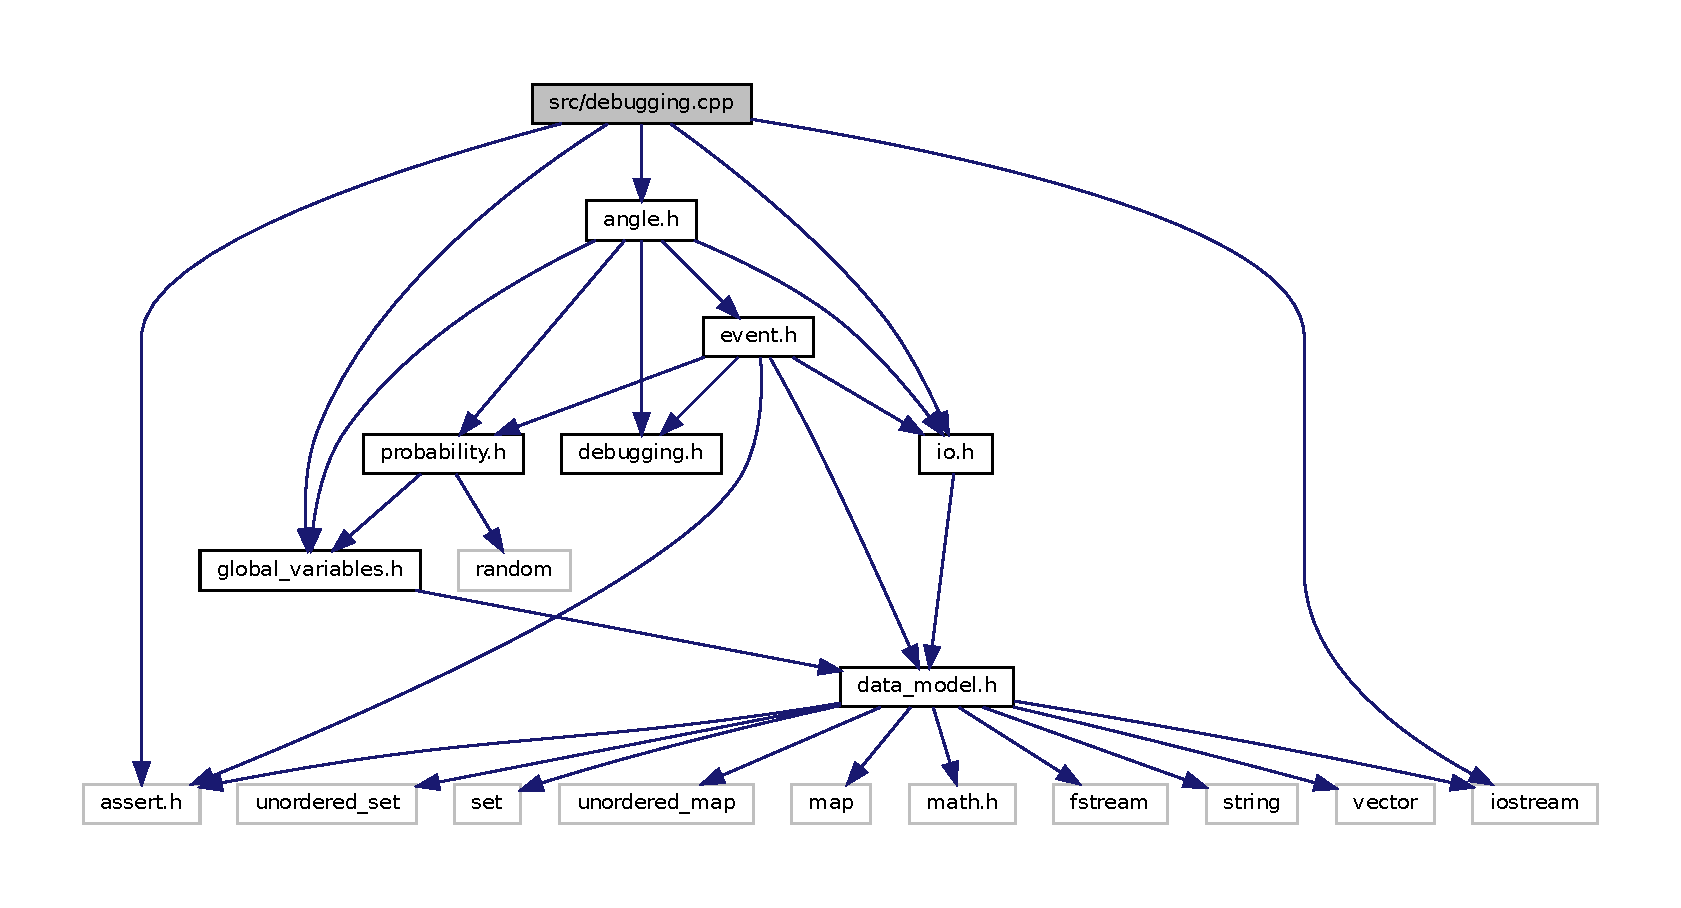
\includegraphics[width=350pt]{d8/d02/debugging_8cpp__incl}
\end{center}
\end{figure}
\subsection*{Functions}
\begin{DoxyCompactItemize}
\item 
int \hyperlink{debugging_8cpp_a8989a80ae48af3b19feed166bb0e2193}{compute\+\_\+n\+\_\+angles} (\hyperlink{structtricl_1_1event__type}{event\+\_\+type} evt, \hyperlink{namespacetricl_a57273122278e8b301844e2a2e1f0742f}{entity} e1, \hyperlink{namespacetricl_a57273122278e8b301844e2a2e1f0742f}{entity} e3, bool print)
\begin{DoxyCompactList}\small\item\em Find the no. \end{DoxyCompactList}\item 
\mbox{\Hypertarget{debugging_8cpp_ad45f6e1ec65e51f87af37e3a100e924b}\label{debugging_8cpp_ad45f6e1ec65e51f87af37e3a100e924b}} 
void \hyperlink{debugging_8cpp_ad45f6e1ec65e51f87af37e3a100e924b}{verify\+\_\+angle\+\_\+consistency} ()
\begin{DoxyCompactList}\small\item\em Verify that data about angles is consistent. \end{DoxyCompactList}\item 
\mbox{\Hypertarget{debugging_8cpp_a75cdc015c7c73360c0e565f4bbea0279}\label{debugging_8cpp_a75cdc015c7c73360c0e565f4bbea0279}} 
void \hyperlink{debugging_8cpp_a75cdc015c7c73360c0e565f4bbea0279}{verify\+\_\+data\+\_\+consistency} ()
\begin{DoxyCompactList}\small\item\em Verify that other data is consistent. \end{DoxyCompactList}\end{DoxyCompactItemize}


\subsection{Detailed Description}
Some stuff only needed for debugging. 



\subsection{Function Documentation}
\mbox{\Hypertarget{debugging_8cpp_a8989a80ae48af3b19feed166bb0e2193}\label{debugging_8cpp_a8989a80ae48af3b19feed166bb0e2193}} 
\index{debugging.\+cpp@{debugging.\+cpp}!compute\+\_\+n\+\_\+angles@{compute\+\_\+n\+\_\+angles}}
\index{compute\+\_\+n\+\_\+angles@{compute\+\_\+n\+\_\+angles}!debugging.\+cpp@{debugging.\+cpp}}
\subsubsection{\texorpdfstring{compute\+\_\+n\+\_\+angles()}{compute\_n\_angles()}}
{\footnotesize\ttfamily int compute\+\_\+n\+\_\+angles (\begin{DoxyParamCaption}\item[{\hyperlink{structtricl_1_1event__type}{event\+\_\+type}}]{evt,  }\item[{\hyperlink{namespacetricl_a57273122278e8b301844e2a2e1f0742f}{entity}}]{e1,  }\item[{\hyperlink{namespacetricl_a57273122278e8b301844e2a2e1f0742f}{entity}}]{e3,  }\item[{bool}]{print }\end{DoxyParamCaption})}



Find the no. 

of angles influencing an event from scratch in order to compare it with the stored no. 
\hypertarget{entity_8cpp}{}\section{src/entity.cpp File Reference}
\label{entity_8cpp}\index{src/entity.\+cpp@{src/entity.\+cpp}}


Handling of entities.  


{\ttfamily \#include $<$iostream$>$}\newline
{\ttfamily \#include $<$math.\+h$>$}\newline
{\ttfamily \#include \char`\"{}global\+\_\+variables.\+h\char`\"{}}\newline
{\ttfamily \#include \char`\"{}entity.\+h\char`\"{}}\newline
{\ttfamily \#include \char`\"{}probability.\+h\char`\"{}}\newline
Include dependency graph for entity.\+cpp\+:\nopagebreak
\begin{figure}[H]
\begin{center}
\leavevmode
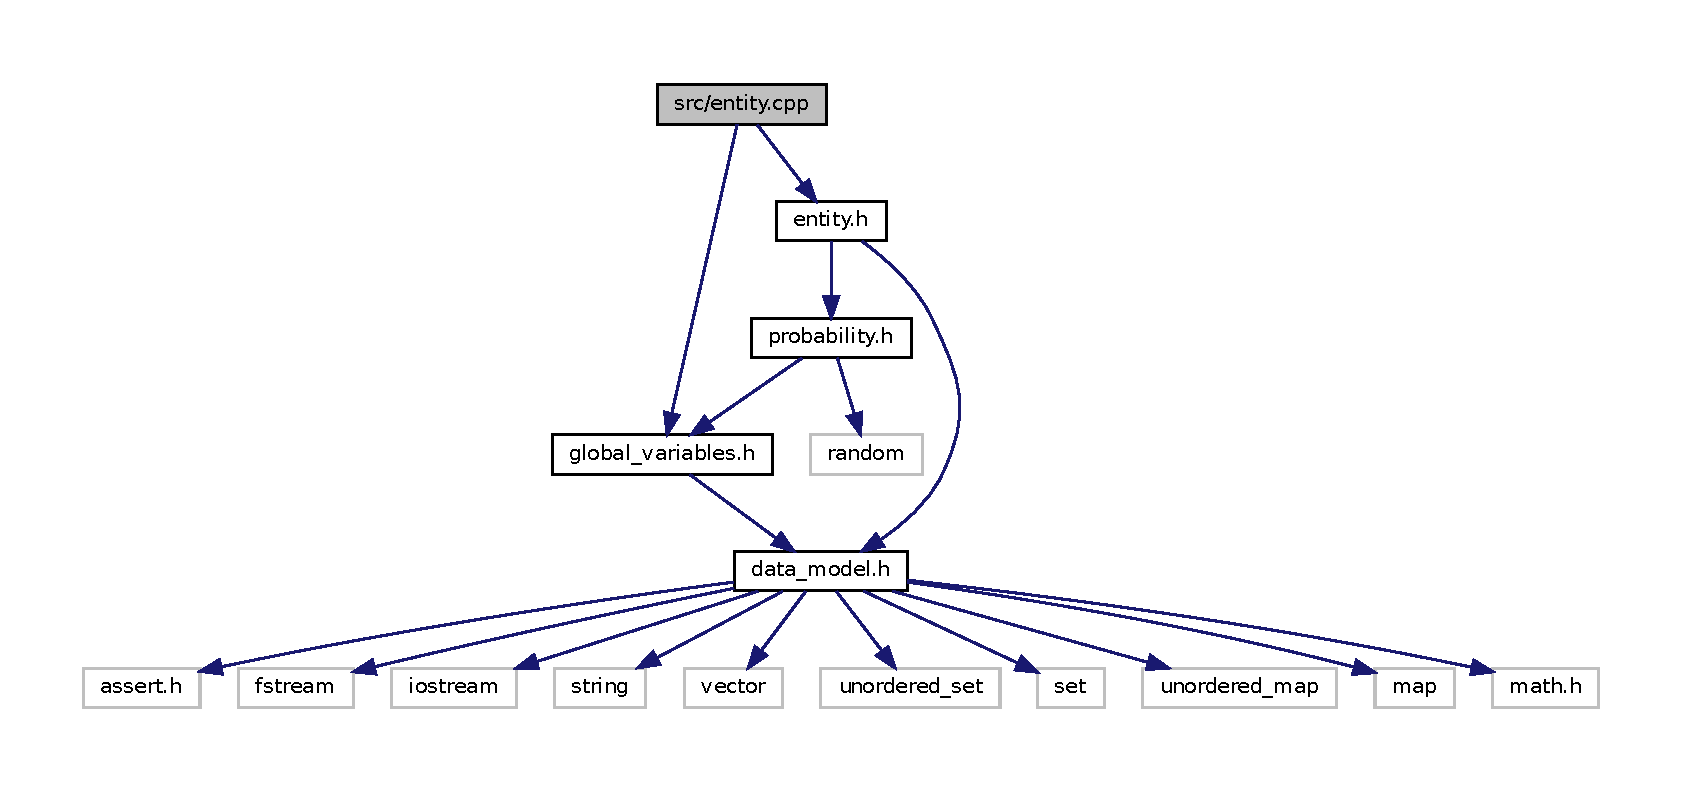
\includegraphics[width=350pt]{d8/d92/entity_8cpp__incl}
\end{center}
\end{figure}
\subsection*{Functions}
\begin{DoxyCompactItemize}
\item 
\hyperlink{namespacetricl_a57273122278e8b301844e2a2e1f0742f}{entity} \hyperlink{entity_8cpp_a0a2d9d57b1737f98889d96db80b44ea4}{add\+\_\+entity} (\hyperlink{namespacetricl_afd4de3aedd5e48cf955f03457386e98f}{entity\+\_\+type} et, string elabel)
\begin{DoxyCompactList}\small\item\em Add a new entity of a specific type. \end{DoxyCompactList}\item 
\hyperlink{namespacetricl_a57273122278e8b301844e2a2e1f0742f}{entity} \hyperlink{entity_8cpp_a98c686b5512ec703bd0da855cd296f24}{random\+\_\+entity} (\hyperlink{namespacetricl_afd4de3aedd5e48cf955f03457386e98f}{entity\+\_\+type} et)
\begin{DoxyCompactList}\small\item\em Return a random entity of a specific type. \end{DoxyCompactList}\end{DoxyCompactItemize}


\subsection{Detailed Description}
Handling of entities. 

\begin{DoxyAuthor}{Author}
Jobst Heitzig, Potsdam Institute for Climate Impact Research, \href{mailto:heitzig@pik-potsdam.de}{\tt heitzig@pik-\/potsdam.\+de} 
\end{DoxyAuthor}
\begin{DoxyDate}{Date}
Mar 30, 2020 
\end{DoxyDate}


\subsection{Function Documentation}
\mbox{\Hypertarget{entity_8cpp_a0a2d9d57b1737f98889d96db80b44ea4}\label{entity_8cpp_a0a2d9d57b1737f98889d96db80b44ea4}} 
\index{entity.\+cpp@{entity.\+cpp}!add\+\_\+entity@{add\+\_\+entity}}
\index{add\+\_\+entity@{add\+\_\+entity}!entity.\+cpp@{entity.\+cpp}}
\subsubsection{\texorpdfstring{add\+\_\+entity()}{add\_entity()}}
{\footnotesize\ttfamily \hyperlink{namespacetricl_a57273122278e8b301844e2a2e1f0742f}{entity} add\+\_\+entity (\begin{DoxyParamCaption}\item[{\hyperlink{namespacetricl_afd4de3aedd5e48cf955f03457386e98f}{entity\+\_\+type}}]{et,  }\item[{string}]{elabel }\end{DoxyParamCaption})}



Add a new entity of a specific type. 

(the entity is not returned) 
\begin{DoxyParams}[1]{Parameters}
\mbox{\tt in}  & {\em et} & entity type of the entity to be generated anew. \\
\hline
\mbox{\tt in}  & {\em elabel} & entity label (if \char`\"{}\char`\"{}, will be generated) \\
\hline
\end{DoxyParams}
\mbox{\Hypertarget{entity_8cpp_a98c686b5512ec703bd0da855cd296f24}\label{entity_8cpp_a98c686b5512ec703bd0da855cd296f24}} 
\index{entity.\+cpp@{entity.\+cpp}!random\+\_\+entity@{random\+\_\+entity}}
\index{random\+\_\+entity@{random\+\_\+entity}!entity.\+cpp@{entity.\+cpp}}
\subsubsection{\texorpdfstring{random\+\_\+entity()}{random\_entity()}}
{\footnotesize\ttfamily \hyperlink{namespacetricl_a57273122278e8b301844e2a2e1f0742f}{entity} random\+\_\+entity (\begin{DoxyParamCaption}\item[{\hyperlink{namespacetricl_afd4de3aedd5e48cf955f03457386e98f}{entity\+\_\+type}}]{et }\end{DoxyParamCaption})}



Return a random entity of a specific type. 

The entity is drawn uniformly at random. 
\begin{DoxyParams}[1]{Parameters}
\mbox{\tt in}  & {\em et} & Entity type of which a random entity is needed \\
\hline
\end{DoxyParams}

\hypertarget{entity_8h}{}\section{src/entity.h File Reference}
\label{entity_8h}\index{src/entity.\+h@{src/entity.\+h}}


Performance-\/critical inline functions for handling of entities.  


{\ttfamily \#include \char`\"{}data\+\_\+model.\+h\char`\"{}}\newline
{\ttfamily \#include \char`\"{}probability.\+h\char`\"{}}\newline
Include dependency graph for entity.\+h\+:\nopagebreak
\begin{figure}[H]
\begin{center}
\leavevmode
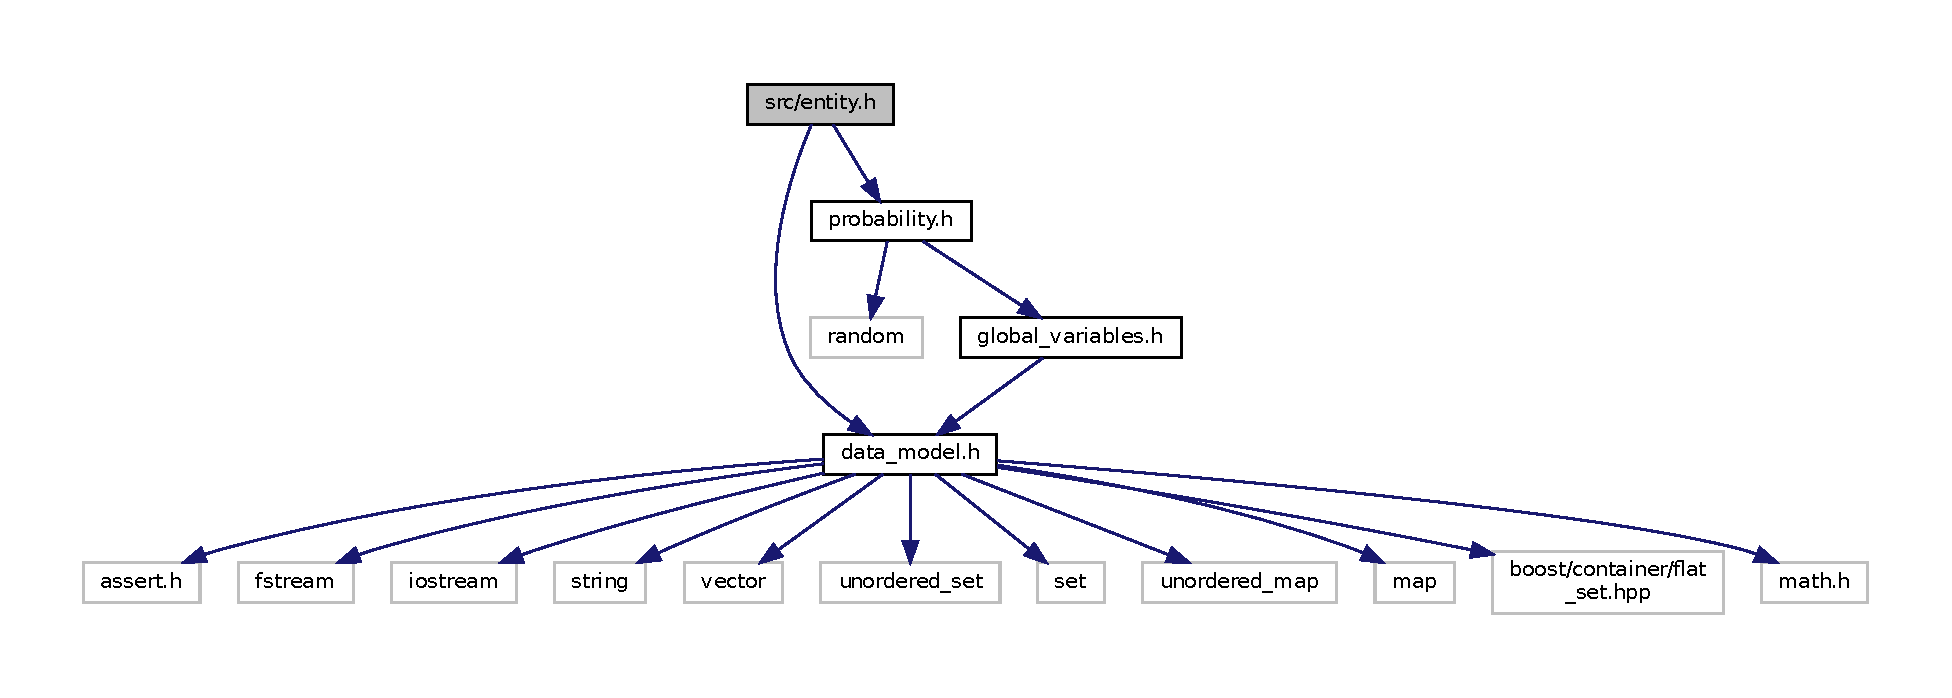
\includegraphics[width=350pt]{d1/ded/entity_8h__incl}
\end{center}
\end{figure}
This graph shows which files directly or indirectly include this file\+:
\nopagebreak
\begin{figure}[H]
\begin{center}
\leavevmode
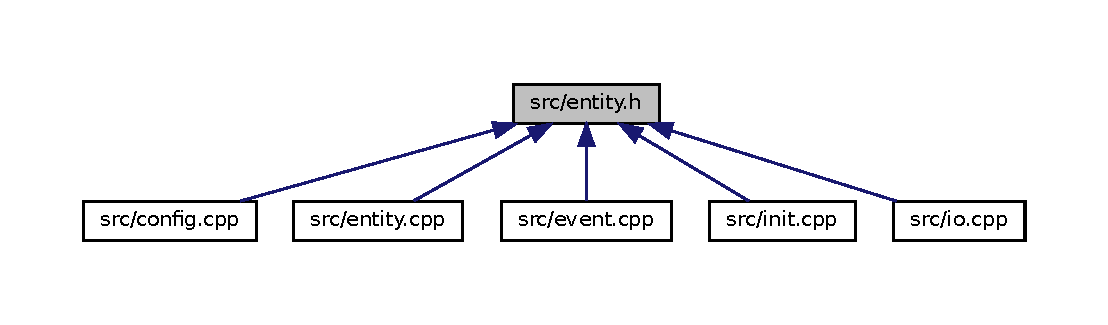
\includegraphics[width=350pt]{d0/d4b/entity_8h__dep__incl}
\end{center}
\end{figure}
\subsection*{Functions}
\begin{DoxyCompactItemize}
\item 
\hyperlink{namespacetricl_a57273122278e8b301844e2a2e1f0742f}{entity} \hyperlink{entity_8h_a63c7b12e1c90def63a1505349df4b3bb}{add\+\_\+entity} (\hyperlink{namespacetricl_afd4de3aedd5e48cf955f03457386e98f}{entity\+\_\+type} et, string \hyperlink{namespacetricl_a77e7daffafa870e5786b344119da9b15}{label})
\begin{DoxyCompactList}\small\item\em Add a new entity of a specific type. \end{DoxyCompactList}\item 
\hyperlink{namespacetricl_a57273122278e8b301844e2a2e1f0742f}{entity} \hyperlink{entity_8h_a98c686b5512ec703bd0da855cd296f24}{random\+\_\+entity} (\hyperlink{namespacetricl_afd4de3aedd5e48cf955f03457386e98f}{entity\+\_\+type} et)
\begin{DoxyCompactList}\small\item\em Return an entity uniformly drawn at random from a specific type. \end{DoxyCompactList}\end{DoxyCompactItemize}


\subsection{Detailed Description}
Performance-\/critical inline functions for handling of entities. 

See \hyperlink{data__model_8h}{data\+\_\+model.\+h} for how a \hyperlink{namespacetricl_a57273122278e8b301844e2a2e1f0742f}{tricl\+::entity} relates to other tricl datatypes. 

\subsection{Function Documentation}
\mbox{\Hypertarget{entity_8h_a63c7b12e1c90def63a1505349df4b3bb}\label{entity_8h_a63c7b12e1c90def63a1505349df4b3bb}} 
\index{entity.\+h@{entity.\+h}!add\+\_\+entity@{add\+\_\+entity}}
\index{add\+\_\+entity@{add\+\_\+entity}!entity.\+h@{entity.\+h}}
\subsubsection{\texorpdfstring{add\+\_\+entity()}{add\_entity()}}
{\footnotesize\ttfamily \hyperlink{namespacetricl_a57273122278e8b301844e2a2e1f0742f}{entity} add\+\_\+entity (\begin{DoxyParamCaption}\item[{\hyperlink{namespacetricl_afd4de3aedd5e48cf955f03457386e98f}{entity\+\_\+type}}]{et,  }\item[{string}]{elabel }\end{DoxyParamCaption})}



Add a new entity of a specific type. 

\begin{DoxyReturn}{Returns}
the new entity 
\end{DoxyReturn}

\begin{DoxyParams}[1]{Parameters}
\mbox{\tt in}  & {\em et} & entity type of the entity to be generated anew. \\
\hline
\mbox{\tt in}  & {\em elabel} & entity label (if \char`\"{}\char`\"{}, will be generated) \\
\hline
\end{DoxyParams}
\mbox{\Hypertarget{entity_8h_a98c686b5512ec703bd0da855cd296f24}\label{entity_8h_a98c686b5512ec703bd0da855cd296f24}} 
\index{entity.\+h@{entity.\+h}!random\+\_\+entity@{random\+\_\+entity}}
\index{random\+\_\+entity@{random\+\_\+entity}!entity.\+h@{entity.\+h}}
\subsubsection{\texorpdfstring{random\+\_\+entity()}{random\_entity()}}
{\footnotesize\ttfamily \hyperlink{namespacetricl_a57273122278e8b301844e2a2e1f0742f}{entity} random\+\_\+entity (\begin{DoxyParamCaption}\item[{\hyperlink{namespacetricl_afd4de3aedd5e48cf955f03457386e98f}{entity\+\_\+type}}]{et }\end{DoxyParamCaption})\hspace{0.3cm}{\ttfamily [inline]}}



Return an entity uniformly drawn at random from a specific type. 

Mainly used in summary events.

\begin{DoxyReturn}{Returns}
the entity 
\end{DoxyReturn}

\begin{DoxyParams}[1]{Parameters}
\mbox{\tt in}  & {\em et} & Entity type of which a random entity is needed \\
\hline
\end{DoxyParams}

\hypertarget{event_8cpp}{}\section{src/event.cpp File Reference}
\label{event_8cpp}\index{src/event.\+cpp@{src/event.\+cpp}}


Handling of events.  


{\ttfamily \#include $<$assert.\+h$>$}\\*
{\ttfamily \#include $<$iostream$>$}\\*
{\ttfamily \#include \char`\"{}debugging.\+h\char`\"{}}\\*
{\ttfamily \#include \char`\"{}data\+\_\+model.\+h\char`\"{}}\\*
{\ttfamily \#include \char`\"{}global\+\_\+variables.\+h\char`\"{}}\\*
{\ttfamily \#include \char`\"{}entity.\+h\char`\"{}}\\*
{\ttfamily \#include \char`\"{}angle.\+h\char`\"{}}\\*
{\ttfamily \#include \char`\"{}link.\+h\char`\"{}}\\*
{\ttfamily \#include \char`\"{}probability.\+h\char`\"{}}\\*
{\ttfamily \#include \char`\"{}event.\+h\char`\"{}}\\*
{\ttfamily \#include \char`\"{}io.\+h\char`\"{}}\\*
Include dependency graph for event.\+cpp\+:
\nopagebreak
\begin{figure}[H]
\begin{center}
\leavevmode
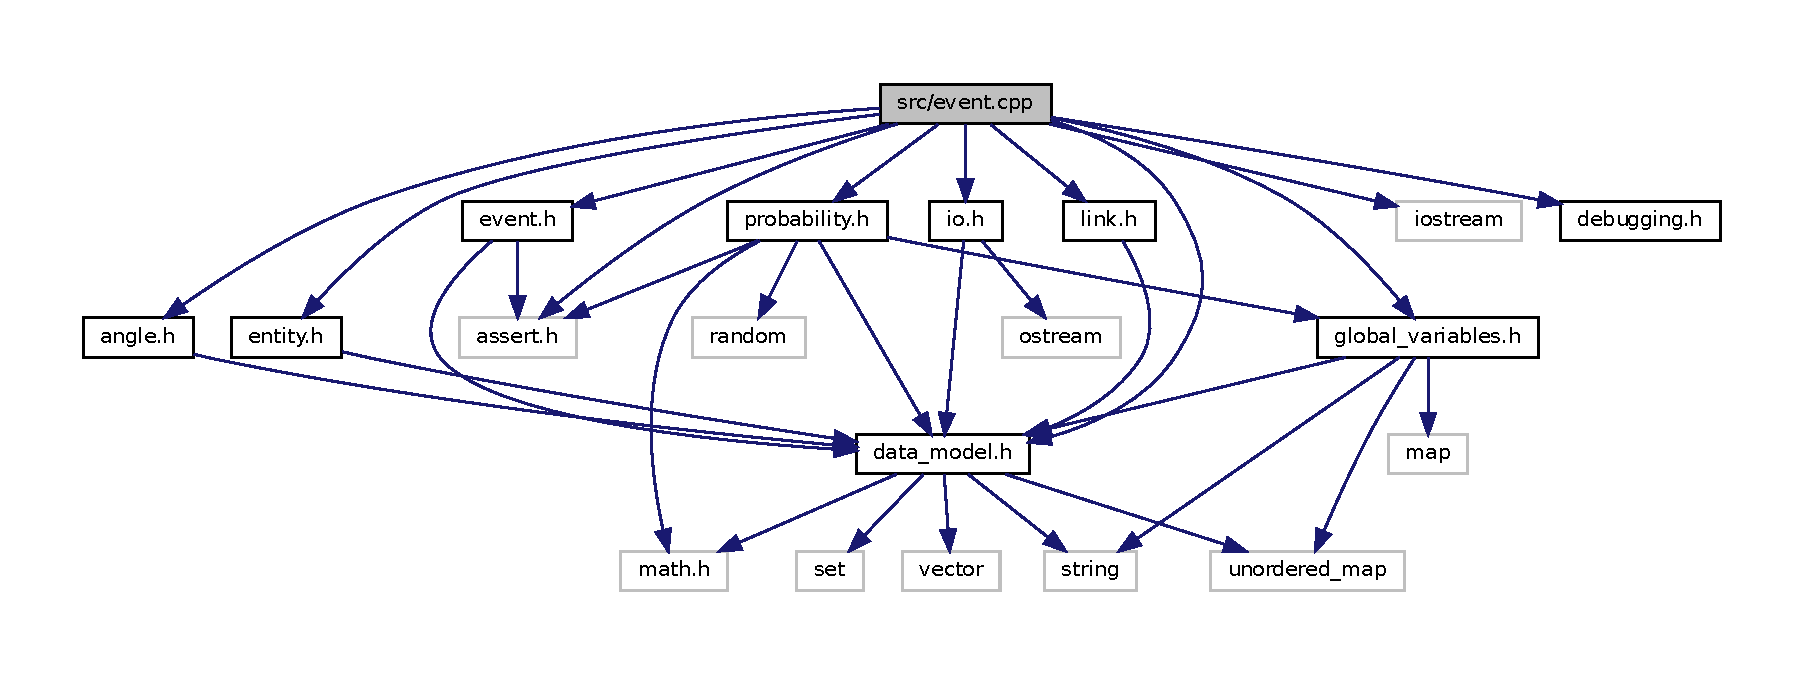
\includegraphics[width=350pt]{d6/d99/event_8cpp__incl}
\end{center}
\end{figure}
\subsection*{Macros}
\begin{DoxyCompactItemize}
\item 
\#define {\bfseries I\+F\+\_\+12}~if (which == 0)\hypertarget{event_8cpp_ac1e75a2e1d58d4f43aaa35324bb26538}{}\label{event_8cpp_ac1e75a2e1d58d4f43aaa35324bb26538}

\item 
\#define {\bfseries I\+F\+\_\+23}~if (which == 1)\hypertarget{event_8cpp_a0add313a6fd3d8fae54c55f125be6f0f}{}\label{event_8cpp_a0add313a6fd3d8fae54c55f125be6f0f}

\end{DoxyCompactItemize}
\subsection*{Functions}
\begin{DoxyCompactItemize}
\item 
bool \hyperlink{event_8cpp_ab8644632b851d99741826fb61fb703bd}{event\+\_\+is\+\_\+scheduled} (\hyperlink{structevent}{event} \&ev, \hyperlink{structevent__data}{event\+\_\+data} $\ast$evd\+\_\+)
\begin{DoxyCompactList}\small\item\em Return whether a future instance of the event is scheduled. \end{DoxyCompactList}\item 
void {\bfseries \+\_\+schedule\+\_\+event} (\hyperlink{structevent}{event} \&ev, \hyperlink{structevent__data}{event\+\_\+data} $\ast$evd\+\_\+, double left\+\_\+tail, double right\+\_\+tail)\hypertarget{event_8cpp_a4048cb830821ab767f91d751e7bd1f37}{}\label{event_8cpp_a4048cb830821ab767f91d751e7bd1f37}

\item 
void {\bfseries schedule\+\_\+event} (\hyperlink{structevent}{event} \&ev, \hyperlink{structevent__data}{event\+\_\+data} $\ast$evd\+\_\+, double left\+\_\+tail, double right\+\_\+tail)\hypertarget{event_8cpp_a269d75ea7ef6f98c60705a062e98f4e0}{}\label{event_8cpp_a269d75ea7ef6f98c60705a062e98f4e0}

\item 
void {\bfseries reschedule\+\_\+event} (\hyperlink{structevent}{event} \&ev, \hyperlink{structevent__data}{event\+\_\+data} $\ast$evd\+\_\+, double left\+\_\+tail, double right\+\_\+tail)\hypertarget{event_8cpp_ad37a5884bb4d210596ad150d6efafed0}{}\label{event_8cpp_ad37a5884bb4d210596ad150d6efafed0}

\item 
void {\bfseries add\+\_\+event} (\hyperlink{structevent}{event} \&ev)\hypertarget{event_8cpp_aef94fa11ff43b90a11586d18670f2700}{}\label{event_8cpp_aef94fa11ff43b90a11586d18670f2700}

\item 
void {\bfseries remove\+\_\+event} (\hyperlink{structevent}{event} \&ev, \hyperlink{structevent__data}{event\+\_\+data} $\ast$evd\+\_\+)\hypertarget{event_8cpp_a55e7ed06ea3900949b3bb7a464670054}{}\label{event_8cpp_a55e7ed06ea3900949b3bb7a464670054}

\item 
void {\bfseries conditionally\+\_\+remove\+\_\+event} (\hyperlink{structevent}{event} \&ev)\hypertarget{event_8cpp_a875f0862466ff1b831fee64602d92d76}{}\label{event_8cpp_a875f0862466ff1b831fee64602d92d76}

\item 
void {\bfseries update\+\_\+adjacent\+\_\+events} (\hyperlink{structevent}{event} \&ev)\hypertarget{event_8cpp_adc013b33a8b8afbb4f75c8c95dc3b93a}{}\label{event_8cpp_adc013b33a8b8afbb4f75c8c95dc3b93a}

\item 
void {\bfseries add\+\_\+reverse\+\_\+event} (\hyperlink{structevent}{event} \&old\+\_\+ev)\hypertarget{event_8cpp_aec4dd06c452378363b04a58a0cfe8f8b}{}\label{event_8cpp_aec4dd06c452378363b04a58a0cfe8f8b}

\item 
void {\bfseries perform\+\_\+event} (\hyperlink{structevent}{event} \&ev)\hypertarget{event_8cpp_af13ceffde477e67e6d9418750ce45107}{}\label{event_8cpp_af13ceffde477e67e6d9418750ce45107}

\item 
bool {\bfseries pop\+\_\+next\+\_\+event} ()\hypertarget{event_8cpp_ad57de4475b376dedfc003a1b09cfece8}{}\label{event_8cpp_ad57de4475b376dedfc003a1b09cfece8}

\end{DoxyCompactItemize}


\subsection{Detailed Description}
Handling of events. 

An event is a tuple \{ec, e1, rat13, e3\} where ec is the event class (E\+C\+\_\+\+E\+ST or E\+C\+\_\+\+T\+E\+RM for establishment or termination of a relationship, E\+C\+\_\+\+A\+CT for the occurrence of an act), e1 and e3 are the affected entities, and rat13 is the relationship or action type.

An event type is a tuple (ec, et1, rat13, et3\} where et1, et3 are two entity types.

An event\textquotesingle{}s variable data (current attempt rate, success probability units, and next scheduled timepoint) is stored in a separate struct of type \hyperlink{structevent__data}{event\+\_\+data}.

\begin{DoxyAuthor}{Author}
Jobst Heitzig, Potsdam Institute for Climate Impact Research, \href{mailto:heitzig@pik-potsdam.de}{\tt heitzig@pik-\/potsdam.\+de} 
\end{DoxyAuthor}
\begin{DoxyDate}{Date}
Mar 30, 2020 
\end{DoxyDate}


\subsection{Function Documentation}
\index{event.\+cpp@{event.\+cpp}!event\+\_\+is\+\_\+scheduled@{event\+\_\+is\+\_\+scheduled}}
\index{event\+\_\+is\+\_\+scheduled@{event\+\_\+is\+\_\+scheduled}!event.\+cpp@{event.\+cpp}}
\subsubsection[{\texorpdfstring{event\+\_\+is\+\_\+scheduled(event \&ev, event\+\_\+data $\ast$evd\+\_\+)}{event_is_scheduled(event &ev, event_data *evd_)}}]{\setlength{\rightskip}{0pt plus 5cm}bool event\+\_\+is\+\_\+scheduled (
\begin{DoxyParamCaption}
\item[{{\bf event} \&}]{ev, }
\item[{{\bf event\+\_\+data} $\ast$}]{evd\+\_\+}
\end{DoxyParamCaption}
)}\hypertarget{event_8cpp_ab8644632b851d99741826fb61fb703bd}{}\label{event_8cpp_ab8644632b851d99741826fb61fb703bd}


Return whether a future instance of the event is scheduled. 


\begin{DoxyParams}[1]{Parameters}
\mbox{\tt in}  & {\em ev} & the event to check, passed by reference for performance \\
\hline
\mbox{\tt in}  & {\em evd\+\_\+} & the corresponding variable event data, passed by pointer for performance \\
\hline
\end{DoxyParams}

\hypertarget{event_8h}{}\section{src/event.h File Reference}
\label{event_8h}\index{src/event.\+h@{src/event.\+h}}


Performance-\/critical inline functions for handling of events.  


{\ttfamily \#include $<$assert.\+h$>$}\newline
{\ttfamily \#include \char`\"{}data\+\_\+model.\+h\char`\"{}}\newline
{\ttfamily \#include \char`\"{}probability.\+h\char`\"{}}\newline
{\ttfamily \#include \char`\"{}io.\+h\char`\"{}}\newline
{\ttfamily \#include \char`\"{}debugging.\+h\char`\"{}}\newline
Include dependency graph for event.\+h\+:\nopagebreak
\begin{figure}[H]
\begin{center}
\leavevmode
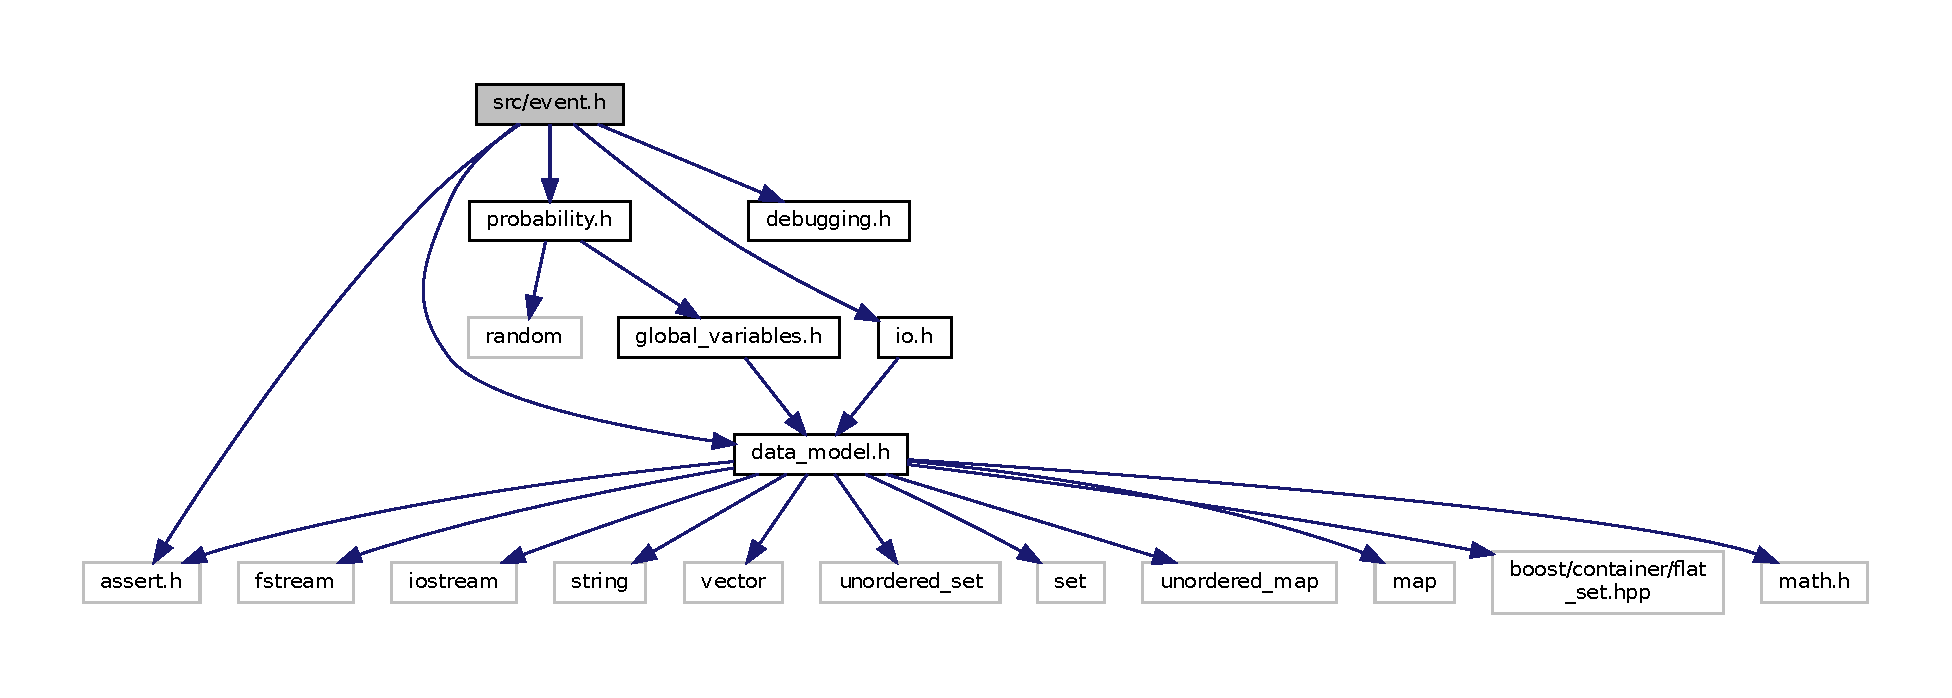
\includegraphics[width=350pt]{d9/d06/event_8h__incl}
\end{center}
\end{figure}
This graph shows which files directly or indirectly include this file\+:\nopagebreak
\begin{figure}[H]
\begin{center}
\leavevmode
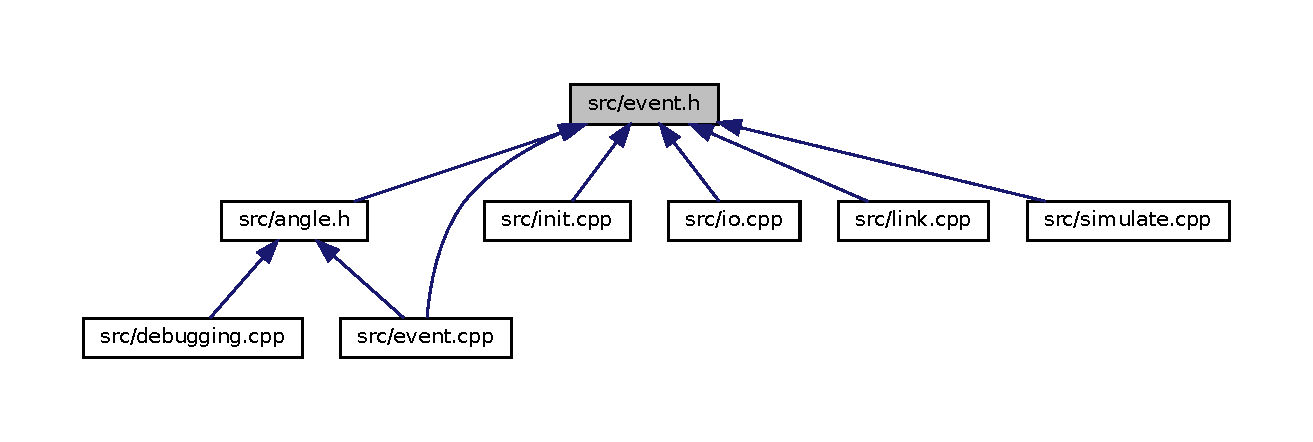
\includegraphics[width=350pt]{d1/d41/event_8h__dep__incl}
\end{center}
\end{figure}
\subsection*{Functions}
\begin{DoxyCompactItemize}
\item 
\mbox{\Hypertarget{event_8h_a5e7ea570ae4eb47e074fe61d3c3f8af7}\label{event_8h_a5e7ea570ae4eb47e074fe61d3c3f8af7}} 
bool {\bfseries event\+\_\+is\+\_\+summary} (const \hyperlink{structtricl_1_1event}{event} \&ev)
\item 
\mbox{\Hypertarget{event_8h_a3566ddb08d205f9df16fec4e6dbc32e3}\label{event_8h_a3566ddb08d205f9df16fec4e6dbc32e3}} 
\hyperlink{namespacetricl_afd4de3aedd5e48cf955f03457386e98f}{entity\+\_\+type} {\bfseries summary\+\_\+et1} (const \hyperlink{structtricl_1_1event}{event} \&ev)
\item 
\mbox{\Hypertarget{event_8h_a0fdd1444b7ca109e06564537ea2446d3}\label{event_8h_a0fdd1444b7ca109e06564537ea2446d3}} 
\hyperlink{namespacetricl_afd4de3aedd5e48cf955f03457386e98f}{entity\+\_\+type} {\bfseries summary\+\_\+et3} (const \hyperlink{structtricl_1_1event}{event} \&ev)
\item 
bool \hyperlink{event_8h_ab8644632b851d99741826fb61fb703bd}{event\+\_\+is\+\_\+scheduled} (\hyperlink{structtricl_1_1event}{event} \&ev, \hyperlink{structtricl_1_1event__data}{event\+\_\+data} $\ast$evd\+\_\+)
\begin{DoxyCompactList}\small\item\em Return whether a future instance of the event is scheduled. \end{DoxyCompactList}\item 
\mbox{\Hypertarget{event_8h_a4048cb830821ab767f91d751e7bd1f37}\label{event_8h_a4048cb830821ab767f91d751e7bd1f37}} 
void {\bfseries \+\_\+schedule\+\_\+event} (\hyperlink{structtricl_1_1event}{event} \&ev, \hyperlink{structtricl_1_1event__data}{event\+\_\+data} $\ast$evd\+\_\+, double left\+\_\+tail, double right\+\_\+tail)
\item 
\mbox{\Hypertarget{event_8h_a269d75ea7ef6f98c60705a062e98f4e0}\label{event_8h_a269d75ea7ef6f98c60705a062e98f4e0}} 
void {\bfseries schedule\+\_\+event} (\hyperlink{structtricl_1_1event}{event} \&ev, \hyperlink{structtricl_1_1event__data}{event\+\_\+data} $\ast$evd\+\_\+, double left\+\_\+tail, double right\+\_\+tail)
\item 
\mbox{\Hypertarget{event_8h_ad37a5884bb4d210596ad150d6efafed0}\label{event_8h_ad37a5884bb4d210596ad150d6efafed0}} 
void {\bfseries reschedule\+\_\+event} (\hyperlink{structtricl_1_1event}{event} \&ev, \hyperlink{structtricl_1_1event__data}{event\+\_\+data} $\ast$evd\+\_\+, double left\+\_\+tail, double right\+\_\+tail)
\item 
void \hyperlink{event_8h_aef94fa11ff43b90a11586d18670f2700}{add\+\_\+event} (\hyperlink{structtricl_1_1event}{event} \&ev)
\begin{DoxyCompactList}\small\item\em Add (and then schedule) an event. \end{DoxyCompactList}\item 
void \hyperlink{event_8h_a55e7ed06ea3900949b3bb7a464670054}{remove\+\_\+event} (\hyperlink{structtricl_1_1event}{event} \&ev, \hyperlink{structtricl_1_1event__data}{event\+\_\+data} $\ast$evd\+\_\+)
\begin{DoxyCompactList}\small\item\em Remove a scheduled event. \end{DoxyCompactList}\item 
void \hyperlink{event_8h_a875f0862466ff1b831fee64602d92d76}{conditionally\+\_\+remove\+\_\+event} (\hyperlink{structtricl_1_1event}{event} \&ev)
\begin{DoxyCompactList}\small\item\em Remove event if scheduled and adjust total effective rate (!). \end{DoxyCompactList}\item 
void \hyperlink{event_8h_adc013b33a8b8afbb4f75c8c95dc3b93a}{update\+\_\+adjacent\+\_\+events} (\hyperlink{structtricl_1_1event}{event} \&ev)
\begin{DoxyCompactList}\small\item\em Update all events which are adjacent to a given event because the event affects angles that might influence them. \end{DoxyCompactList}\item 
void \hyperlink{event_8h_aec4dd06c452378363b04a58a0cfe8f8b}{add\+\_\+reverse\+\_\+event} (\hyperlink{structtricl_1_1event}{event} \&old\+\_\+ev)
\begin{DoxyCompactList}\small\item\em Add the reverse event of a just performed event. \end{DoxyCompactList}\item 
void \hyperlink{event_8h_abd0fec822d726403436f1bdad4aa7b51}{perform\+\_\+event} (\hyperlink{structtricl_1_1event}{event} \&ev, \hyperlink{structtricl_1_1event__data}{event\+\_\+data} $\ast$evd\+\_\+)
\begin{DoxyCompactList}\small\item\em Perform an event (usually the current event). \end{DoxyCompactList}\item 
bool \hyperlink{event_8h_ad57de4475b376dedfc003a1b09cfece8}{pop\+\_\+next\+\_\+event} ()
\begin{DoxyCompactList}\small\item\em Find the next occurring event. \end{DoxyCompactList}\end{DoxyCompactItemize}


\subsection{Detailed Description}
Performance-\/critical inline functions for handling of events. 

See \hyperlink{data__model_8h}{data\+\_\+model.\+h} for how a \hyperlink{structtricl_1_1event}{tricl\+::event} relates to other tricl datatypes. 

\subsection{Function Documentation}
\mbox{\Hypertarget{event_8h_aef94fa11ff43b90a11586d18670f2700}\label{event_8h_aef94fa11ff43b90a11586d18670f2700}} 
\index{event.\+h@{event.\+h}!add\+\_\+event@{add\+\_\+event}}
\index{add\+\_\+event@{add\+\_\+event}!event.\+h@{event.\+h}}
\subsubsection{\texorpdfstring{add\+\_\+event()}{add\_event()}}
{\footnotesize\ttfamily void add\+\_\+event (\begin{DoxyParamCaption}\item[{\hyperlink{structtricl_1_1event}{event} \&}]{ev }\end{DoxyParamCaption})}



Add (and then schedule) an event. 

To determine the effective rate of the event, all influencing angles must be identified.

This is a performance-\/critical function, using a large share of the model\textquotesingle{}s C\+PU time. 
\begin{DoxyParams}[1]{Parameters}
\mbox{\tt in}  & {\em ev} & the event to be added \\
\hline
\end{DoxyParams}
\mbox{\Hypertarget{event_8h_aec4dd06c452378363b04a58a0cfe8f8b}\label{event_8h_aec4dd06c452378363b04a58a0cfe8f8b}} 
\index{event.\+h@{event.\+h}!add\+\_\+reverse\+\_\+event@{add\+\_\+reverse\+\_\+event}}
\index{add\+\_\+reverse\+\_\+event@{add\+\_\+reverse\+\_\+event}!event.\+h@{event.\+h}}
\subsubsection{\texorpdfstring{add\+\_\+reverse\+\_\+event()}{add\_reverse\_event()}}
{\footnotesize\ttfamily void add\+\_\+reverse\+\_\+event (\begin{DoxyParamCaption}\item[{\hyperlink{structtricl_1_1event}{event} \&}]{old\+\_\+ev }\end{DoxyParamCaption})}



Add the reverse event of a just performed event. 

(the reverse of E\+C\+\_\+\+E\+ST is E\+C\+\_\+\+T\+E\+RM and vice versa, E\+C\+\_\+\+A\+CT has no reverse) 
\begin{DoxyParams}[1]{Parameters}
\mbox{\tt in}  & {\em old\+\_\+ev} & the just performed event whose reverse shall be added \\
\hline
\end{DoxyParams}
\mbox{\Hypertarget{event_8h_a875f0862466ff1b831fee64602d92d76}\label{event_8h_a875f0862466ff1b831fee64602d92d76}} 
\index{event.\+h@{event.\+h}!conditionally\+\_\+remove\+\_\+event@{conditionally\+\_\+remove\+\_\+event}}
\index{conditionally\+\_\+remove\+\_\+event@{conditionally\+\_\+remove\+\_\+event}!event.\+h@{event.\+h}}
\subsubsection{\texorpdfstring{conditionally\+\_\+remove\+\_\+event()}{conditionally\_remove\_event()}}
{\footnotesize\ttfamily void conditionally\+\_\+remove\+\_\+event (\begin{DoxyParamCaption}\item[{\hyperlink{structtricl_1_1event}{event} \&}]{ev }\end{DoxyParamCaption})}



Remove event if scheduled and adjust total effective rate (!). 


\begin{DoxyParams}[1]{Parameters}
\mbox{\tt in}  & {\em ev} & the event to remove \\
\hline
\end{DoxyParams}
\mbox{\Hypertarget{event_8h_ab8644632b851d99741826fb61fb703bd}\label{event_8h_ab8644632b851d99741826fb61fb703bd}} 
\index{event.\+h@{event.\+h}!event\+\_\+is\+\_\+scheduled@{event\+\_\+is\+\_\+scheduled}}
\index{event\+\_\+is\+\_\+scheduled@{event\+\_\+is\+\_\+scheduled}!event.\+h@{event.\+h}}
\subsubsection{\texorpdfstring{event\+\_\+is\+\_\+scheduled()}{event\_is\_scheduled()}}
{\footnotesize\ttfamily bool event\+\_\+is\+\_\+scheduled (\begin{DoxyParamCaption}\item[{\hyperlink{structtricl_1_1event}{event} \&}]{ev,  }\item[{\hyperlink{structtricl_1_1event__data}{event\+\_\+data} $\ast$}]{evd\+\_\+ }\end{DoxyParamCaption})\hspace{0.3cm}{\ttfamily [inline]}}



Return whether a future instance of the event is scheduled. 


\begin{DoxyParams}[1]{Parameters}
\mbox{\tt in}  & {\em ev} & the event to check, passed by reference for performance \\
\hline
\mbox{\tt in}  & {\em evd\+\_\+} & the corresponding variable event data, passed by pointer for performance \\
\hline
\end{DoxyParams}
\mbox{\Hypertarget{event_8h_abd0fec822d726403436f1bdad4aa7b51}\label{event_8h_abd0fec822d726403436f1bdad4aa7b51}} 
\index{event.\+h@{event.\+h}!perform\+\_\+event@{perform\+\_\+event}}
\index{perform\+\_\+event@{perform\+\_\+event}!event.\+h@{event.\+h}}
\subsubsection{\texorpdfstring{perform\+\_\+event()}{perform\_event()}}
{\footnotesize\ttfamily void perform\+\_\+event (\begin{DoxyParamCaption}\item[{\hyperlink{structtricl_1_1event}{event} \&}]{ev,  }\item[{\hyperlink{structtricl_1_1event__data}{event\+\_\+data} $\ast$}]{evd\+\_\+ }\end{DoxyParamCaption})}



Perform an event (usually the current event). 

In this function, the order of updates is crucial for keeping data consistent\+: add reverse event, add or remove link, update adjacent events.

If the relationship or action type rat13 is asymmetric and has a named inverse rat31, then also do the same things for the companion event that deals with the inverse link e3--rat31--$>$e1. 
\begin{DoxyParams}[1]{Parameters}
\mbox{\tt in}  & {\em ev} & the event to perform \\
\hline
\mbox{\tt in}  & {\em evd\+\_\+} & ptr to the corresponding event data \\
\hline
\end{DoxyParams}
\mbox{\Hypertarget{event_8h_ad57de4475b376dedfc003a1b09cfece8}\label{event_8h_ad57de4475b376dedfc003a1b09cfece8}} 
\index{event.\+h@{event.\+h}!pop\+\_\+next\+\_\+event@{pop\+\_\+next\+\_\+event}}
\index{pop\+\_\+next\+\_\+event@{pop\+\_\+next\+\_\+event}!event.\+h@{event.\+h}}
\subsubsection{\texorpdfstring{pop\+\_\+next\+\_\+event()}{pop\_next\_event()}}
{\footnotesize\ttfamily bool pop\+\_\+next\+\_\+event (\begin{DoxyParamCaption}{ }\end{DoxyParamCaption})}



Find the next occurring event. 

Basically, find the minimum-\/time entry in the ordered map of scheduled events. (If that is a summary event, draw entities for it at random and check whether it succeeds; if it doesn\textquotesingle{}t succeed, repeat.)

\begin{DoxyReturn}{Returns}
whether an event was found that happens before the end of the simulation. 
\end{DoxyReturn}
\mbox{\Hypertarget{event_8h_a55e7ed06ea3900949b3bb7a464670054}\label{event_8h_a55e7ed06ea3900949b3bb7a464670054}} 
\index{event.\+h@{event.\+h}!remove\+\_\+event@{remove\+\_\+event}}
\index{remove\+\_\+event@{remove\+\_\+event}!event.\+h@{event.\+h}}
\subsubsection{\texorpdfstring{remove\+\_\+event()}{remove\_event()}}
{\footnotesize\ttfamily void remove\+\_\+event (\begin{DoxyParamCaption}\item[{\hyperlink{structtricl_1_1event}{event} \&}]{ev,  }\item[{\hyperlink{structtricl_1_1event__data}{event\+\_\+data} $\ast$}]{evd\+\_\+ }\end{DoxyParamCaption})}



Remove a scheduled event. 


\begin{DoxyParams}[1]{Parameters}
\mbox{\tt in}  & {\em ev} & the event to remove \\
\hline
\mbox{\tt in}  & {\em evd\+\_\+} & its data \\
\hline
\end{DoxyParams}
\mbox{\Hypertarget{event_8h_adc013b33a8b8afbb4f75c8c95dc3b93a}\label{event_8h_adc013b33a8b8afbb4f75c8c95dc3b93a}} 
\index{event.\+h@{event.\+h}!update\+\_\+adjacent\+\_\+events@{update\+\_\+adjacent\+\_\+events}}
\index{update\+\_\+adjacent\+\_\+events@{update\+\_\+adjacent\+\_\+events}!event.\+h@{event.\+h}}
\subsubsection{\texorpdfstring{update\+\_\+adjacent\+\_\+events()}{update\_adjacent\_events()}}
{\footnotesize\ttfamily void update\+\_\+adjacent\+\_\+events (\begin{DoxyParamCaption}\item[{\hyperlink{structtricl_1_1event}{event} \&}]{ev }\end{DoxyParamCaption})}



Update all events which are adjacent to a given event because the event affects angles that might influence them. 


\begin{DoxyParams}[1]{Parameters}
\mbox{\tt in}  & {\em ev} & the event whose adjacent events may need update \\
\hline
\end{DoxyParams}

\hypertarget{global__variables_8h}{}\section{src/global\+\_\+variables.h File Reference}
\label{global__variables_8h}\index{src/global\+\_\+variables.\+h@{src/global\+\_\+variables.\+h}}


Definition of global data storage.  


{\ttfamily \#include \char`\"{}data\+\_\+model.\+h\char`\"{}}\newline
Include dependency graph for global\+\_\+variables.\+h\+:\nopagebreak
\begin{figure}[H]
\begin{center}
\leavevmode
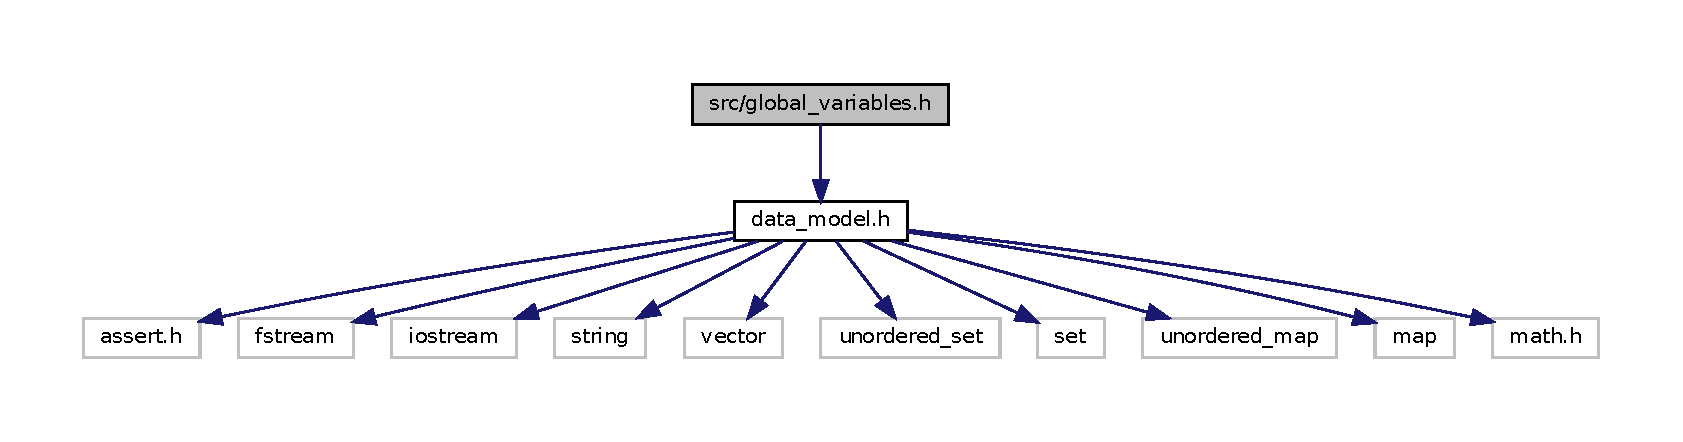
\includegraphics[width=350pt]{d1/d21/global__variables_8h__incl}
\end{center}
\end{figure}
This graph shows which files directly or indirectly include this file\+:
\nopagebreak
\begin{figure}[H]
\begin{center}
\leavevmode
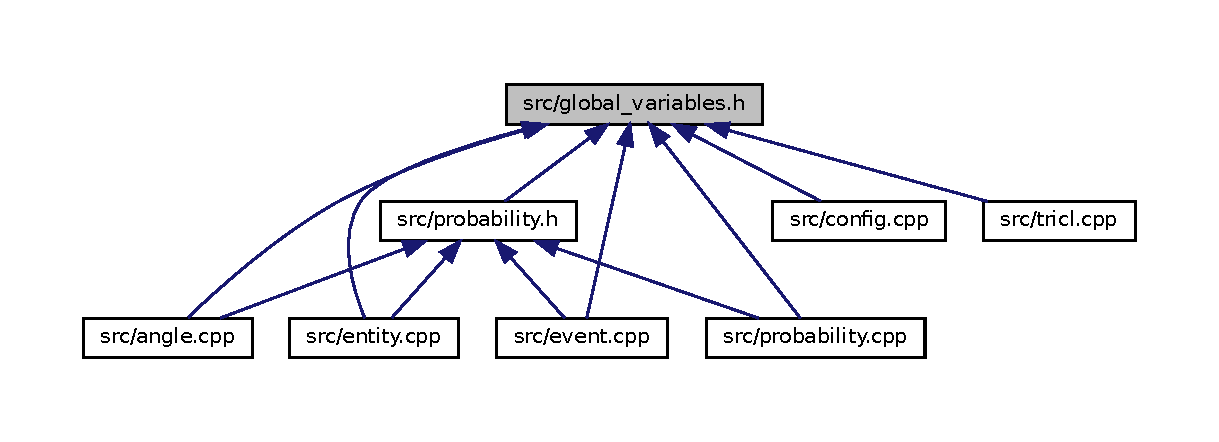
\includegraphics[width=350pt]{de/dbc/global__variables_8h__dep__incl}
\end{center}
\end{figure}
\subsection*{Macros}
\begin{DoxyCompactItemize}
\item 
\mbox{\Hypertarget{global__variables_8h_a20bd8e3d0c96b4a292dc541550fb0d09}\label{global__variables_8h_a20bd8e3d0c96b4a292dc541550fb0d09}} 
\#define {\bfseries C\+O\+U\+N\+T\+\_\+\+A\+L\+L\+\_\+\+A\+N\+G\+L\+ES}~false
\end{DoxyCompactItemize}
\subsection*{Variables}
\begin{DoxyCompactItemize}
\item 
\mbox{\Hypertarget{global__variables_8h_a7153b9485cb42fcae606513208517a6b}\label{global__variables_8h_a7153b9485cb42fcae606513208517a6b}} 
unordered\+\_\+set$<$ \hyperlink{namespacetricl_a57273122278e8b301844e2a2e1f0742f}{entity} $>$ \hyperlink{global__variables_8h_a7153b9485cb42fcae606513208517a6b}{es}
\begin{DoxyCompactList}\small\item\em Set of all entities. \end{DoxyCompactList}\item 
\mbox{\Hypertarget{global__variables_8h_aca8167edc3c91cb84c829dd88f75c7b4}\label{global__variables_8h_aca8167edc3c91cb84c829dd88f75c7b4}} 
\hyperlink{namespacetricl_a57273122278e8b301844e2a2e1f0742f}{entity} \hyperlink{global__variables_8h_aca8167edc3c91cb84c829dd88f75c7b4}{max\+\_\+e}
\begin{DoxyCompactList}\small\item\em Largest entity id in use. \end{DoxyCompactList}\item 
\mbox{\Hypertarget{global__variables_8h_a5575d3ad7f54cb040bf940234988f10c}\label{global__variables_8h_a5575d3ad7f54cb040bf940234988f10c}} 
\hyperlink{namespacetricl_afd4de3aedd5e48cf955f03457386e98f}{entity\+\_\+type} \hyperlink{global__variables_8h_a5575d3ad7f54cb040bf940234988f10c}{e2et} \mbox{[}\hyperlink{data__model_8h_acaa7fd772f80b3066211e5eb6e29ed91}{M\+A\+X\+\_\+\+N\+\_\+E}\mbox{]}
\begin{DoxyCompactList}\small\item\em Entity type by entity (stored in an array for performance) \end{DoxyCompactList}\item 
\mbox{\Hypertarget{global__variables_8h_afde1d602246c7190d16eb890ee87f35b}\label{global__variables_8h_afde1d602246c7190d16eb890ee87f35b}} 
unordered\+\_\+map$<$ \hyperlink{namespacetricl_afd4de3aedd5e48cf955f03457386e98f}{entity\+\_\+type}, vector$<$ \hyperlink{namespacetricl_a57273122278e8b301844e2a2e1f0742f}{entity} $>$ $>$ \hyperlink{global__variables_8h_afde1d602246c7190d16eb890ee87f35b}{et2es}
\begin{DoxyCompactList}\small\item\em Inverse of e2et. \end{DoxyCompactList}\item 
\mbox{\Hypertarget{global__variables_8h_a1d4d2e1edc14bccb896b5dd715cba4a6}\label{global__variables_8h_a1d4d2e1edc14bccb896b5dd715cba4a6}} 
unordered\+\_\+map$<$ \hyperlink{namespacetricl_a57273122278e8b301844e2a2e1f0742f}{entity}, \hyperlink{namespacetricl_a77e7daffafa870e5786b344119da9b15}{label} $>$ \hyperlink{global__variables_8h_a1d4d2e1edc14bccb896b5dd715cba4a6}{e2label}
\begin{DoxyCompactList}\small\item\em Labels of entities. \end{DoxyCompactList}\item 
\mbox{\Hypertarget{global__variables_8h_a3e3cf64afa14be51e4752ebe0e78d8b4}\label{global__variables_8h_a3e3cf64afa14be51e4752ebe0e78d8b4}} 
unordered\+\_\+map$<$ string, \hyperlink{namespacetricl_a57273122278e8b301844e2a2e1f0742f}{entity} $>$ \hyperlink{global__variables_8h_a3e3cf64afa14be51e4752ebe0e78d8b4}{label2e}
\begin{DoxyCompactList}\small\item\em Inverse map of \hyperlink{global__variables_8h_a1d4d2e1edc14bccb896b5dd715cba4a6}{e2label}. \end{DoxyCompactList}\item 
string \hyperlink{global__variables_8h_a6ff215d62218bc381c50ab2e7ef4731d}{config\+\_\+yaml\+\_\+filename}
\begin{DoxyCompactList}\small\item\em Name of (or path to) main config file. \end{DoxyCompactList}\item 
\mbox{\Hypertarget{global__variables_8h_ab3f078684998b83967d507d0f453f454}\label{global__variables_8h_ab3f078684998b83967d507d0f453f454}} 
bool \hyperlink{global__variables_8h_ab3f078684998b83967d507d0f453f454}{verbose}
\begin{DoxyCompactList}\small\item\em Whether to output more detailed information. \end{DoxyCompactList}\item 
\mbox{\Hypertarget{global__variables_8h_ae4426f467d61ae456b95844d4d9c2dcd}\label{global__variables_8h_ae4426f467d61ae456b95844d4d9c2dcd}} 
bool \hyperlink{global__variables_8h_ae4426f467d61ae456b95844d4d9c2dcd}{quiet}
\begin{DoxyCompactList}\small\item\em Whether to suppress most output. \end{DoxyCompactList}\item 
\mbox{\Hypertarget{global__variables_8h_a398527b3e9e358c345c5047b16871957}\label{global__variables_8h_a398527b3e9e358c345c5047b16871957}} 
bool \hyperlink{global__variables_8h_a398527b3e9e358c345c5047b16871957}{debug}
\begin{DoxyCompactList}\small\item\em Whether to output debug messages. \end{DoxyCompactList}\item 
\mbox{\Hypertarget{global__variables_8h_af960657d113135c47b4e0ed4536930c0}\label{global__variables_8h_af960657d113135c47b4e0ed4536930c0}} 
string \hyperlink{global__variables_8h_af960657d113135c47b4e0ed4536930c0}{diagram\+\_\+fileprefix}
\begin{DoxyCompactList}\small\item\em Prefix of name of (or path to) generated diagram files. \end{DoxyCompactList}\item 
\mbox{\Hypertarget{global__variables_8h_a61e4a08c5309d5cd9538ce9654bdb9e9}\label{global__variables_8h_a61e4a08c5309d5cd9538ce9654bdb9e9}} 
\hyperlink{namespacetricl_a720ff6a29f998e11e1d3622fc8df64b1}{timepoint} \hyperlink{global__variables_8h_a61e4a08c5309d5cd9538ce9654bdb9e9}{max\+\_\+t}
\begin{DoxyCompactList}\small\item\em Maximal model time to simulate until. \end{DoxyCompactList}\item 
\mbox{\Hypertarget{global__variables_8h_a921a3c48e5eda75a9944e3d8fdecc826}\label{global__variables_8h_a921a3c48e5eda75a9944e3d8fdecc826}} 
long int \hyperlink{global__variables_8h_a921a3c48e5eda75a9944e3d8fdecc826}{max\+\_\+n\+\_\+events}
\begin{DoxyCompactList}\small\item\em Max. no. events to simulate before stopping. \end{DoxyCompactList}\item 
\mbox{\Hypertarget{global__variables_8h_abb3c5a016eb55b340002c5da33a16714}\label{global__variables_8h_abb3c5a016eb55b340002c5da33a16714}} 
unsigned \hyperlink{global__variables_8h_abb3c5a016eb55b340002c5da33a16714}{seed}
\begin{DoxyCompactList}\small\item\em Random seed (if 0, generate a random seed) \end{DoxyCompactList}\item 
\mbox{\Hypertarget{global__variables_8h_a113f3c013371a7bc91273d8821d8710d}\label{global__variables_8h_a113f3c013371a7bc91273d8821d8710d}} 
unordered\+\_\+map$<$ \hyperlink{namespacetricl_a2d01894944fb58a8fedc0912a48d13f8}{relationship\+\_\+or\+\_\+action\+\_\+type}, string $>$ \hyperlink{global__variables_8h_a113f3c013371a7bc91273d8821d8710d}{gexf\+\_\+filename}
\begin{DoxyCompactList}\small\item\em Names of (or paths to) generated gexf (or gexf.\+gz) files by relationship or action type. \end{DoxyCompactList}\item 
\mbox{\Hypertarget{global__variables_8h_a1b14b11720f5396f884aba602cc42602}\label{global__variables_8h_a1b14b11720f5396f884aba602cc42602}} 
unordered\+\_\+map$<$ \hyperlink{namespacetricl_afd4de3aedd5e48cf955f03457386e98f}{entity\+\_\+type}, \hyperlink{namespacetricl_a77e7daffafa870e5786b344119da9b15}{label} $>$ \hyperlink{global__variables_8h_a1b14b11720f5396f884aba602cc42602}{et2label}
\begin{DoxyCompactList}\small\item\em Entity type labels (typically nouns) \end{DoxyCompactList}\item 
\mbox{\Hypertarget{global__variables_8h_a4ad1375a3f0b5760ef4861ef35ac7f25}\label{global__variables_8h_a4ad1375a3f0b5760ef4861ef35ac7f25}} 
unordered\+\_\+map$<$ string, \hyperlink{namespacetricl_afd4de3aedd5e48cf955f03457386e98f}{entity\+\_\+type} $>$ \hyperlink{global__variables_8h_a4ad1375a3f0b5760ef4861ef35ac7f25}{label2et}
\begin{DoxyCompactList}\small\item\em Inverse map of \hyperlink{global__variables_8h_a1b14b11720f5396f884aba602cc42602}{et2label}. \end{DoxyCompactList}\item 
\mbox{\Hypertarget{global__variables_8h_aba5a0104caf66faf04d0e2f4491415fb}\label{global__variables_8h_aba5a0104caf66faf04d0e2f4491415fb}} 
unordered\+\_\+map$<$ \hyperlink{namespacetricl_afd4de3aedd5e48cf955f03457386e98f}{entity\+\_\+type}, \hyperlink{namespacetricl_a57273122278e8b301844e2a2e1f0742f}{entity} $>$ \hyperlink{global__variables_8h_aba5a0104caf66faf04d0e2f4491415fb}{et2n}
\begin{DoxyCompactList}\small\item\em No. of entities by type. \end{DoxyCompactList}\item 
\mbox{\Hypertarget{global__variables_8h_a41e5e4e1e8384638199deff086cbe4ad}\label{global__variables_8h_a41e5e4e1e8384638199deff086cbe4ad}} 
int \hyperlink{global__variables_8h_a41e5e4e1e8384638199deff086cbe4ad}{n\+\_\+rats}
\begin{DoxyCompactList}\small\item\em No. of distinct relationship or action types. \end{DoxyCompactList}\item 
\mbox{\Hypertarget{global__variables_8h_a16775be180de048f5d158cf6c18af175}\label{global__variables_8h_a16775be180de048f5d158cf6c18af175}} 
unordered\+\_\+map$<$ \hyperlink{namespacetricl_a2d01894944fb58a8fedc0912a48d13f8}{relationship\+\_\+or\+\_\+action\+\_\+type}, \hyperlink{namespacetricl_a77e7daffafa870e5786b344119da9b15}{label} $>$ \hyperlink{global__variables_8h_a16775be180de048f5d158cf6c18af175}{rat2label}
\begin{DoxyCompactList}\small\item\em Relationship or action type labels (typically verbs in the 3rd person singular, or math symbols) \end{DoxyCompactList}\item 
\mbox{\Hypertarget{global__variables_8h_a1b29491c10222b82a8ac3f8241aa27a8}\label{global__variables_8h_a1b29491c10222b82a8ac3f8241aa27a8}} 
unordered\+\_\+map$<$ string, \hyperlink{namespacetricl_a2d01894944fb58a8fedc0912a48d13f8}{relationship\+\_\+or\+\_\+action\+\_\+type} $>$ \hyperlink{global__variables_8h_a1b29491c10222b82a8ac3f8241aa27a8}{label2rat}
\begin{DoxyCompactList}\small\item\em Inverse map of \hyperlink{global__variables_8h_a1b29491c10222b82a8ac3f8241aa27a8}{label2rat}. \end{DoxyCompactList}\item 
\mbox{\Hypertarget{global__variables_8h_acb03df27c0aec975d0d0a27e21f9b956}\label{global__variables_8h_acb03df27c0aec975d0d0a27e21f9b956}} 
unordered\+\_\+map$<$ \hyperlink{namespacetricl_a2d01894944fb58a8fedc0912a48d13f8}{relationship\+\_\+or\+\_\+action\+\_\+type}, bool $>$ \hyperlink{global__variables_8h_acb03df27c0aec975d0d0a27e21f9b956}{r\+\_\+is\+\_\+action\+\_\+type}
\begin{DoxyCompactList}\small\item\em Whether relationship or action type is an action type (not implemented yet) \end{DoxyCompactList}\item 
\mbox{\Hypertarget{global__variables_8h_a698aaa515390777326d52ab118c9f1fe}\label{global__variables_8h_a698aaa515390777326d52ab118c9f1fe}} 
unordered\+\_\+map$<$ \hyperlink{namespacetricl_a2d01894944fb58a8fedc0912a48d13f8}{relationship\+\_\+or\+\_\+action\+\_\+type}, \hyperlink{namespacetricl_a2d01894944fb58a8fedc0912a48d13f8}{relationship\+\_\+or\+\_\+action\+\_\+type} $>$ \hyperlink{global__variables_8h_a698aaa515390777326d52ab118c9f1fe}{rat2inv}
\begin{DoxyCompactList}\small\item\em Inverse type of a relationship or action type (e.\+g. the inverse of \char`\"{}follows\char`\"{} would be \char`\"{}is followed by\char`\"{}, the inverse of \char`\"{}meets\char`\"{} would be \char`\"{}meets\char`\"{}). If N\+O\+\_\+\+R\+AT, inverse has no individual label. \end{DoxyCompactList}\item 
\mbox{\Hypertarget{global__variables_8h_afe42a9a97fc8e959183c94fc333f2331}\label{global__variables_8h_afe42a9a97fc8e959183c94fc333f2331}} 
set$<$ \hyperlink{structtricl_1_1link}{link} $>$ \hyperlink{global__variables_8h_afe42a9a97fc8e959183c94fc333f2331}{initial\+\_\+links}
\begin{DoxyCompactList}\small\item\em Set of named initial links. \end{DoxyCompactList}\item 
\mbox{\Hypertarget{global__variables_8h_ac3d91d4eef87cfaf1371a698513533ba}\label{global__variables_8h_ac3d91d4eef87cfaf1371a698513533ba}} 
unordered\+\_\+map$<$ \hyperlink{namespacetricl_afd4de3aedd5e48cf955f03457386e98f}{entity\+\_\+type}, int $>$ \hyperlink{global__variables_8h_ac3d91d4eef87cfaf1371a698513533ba}{et2n\+\_\+blocks}
\begin{DoxyCompactList}\small\item\em No. of blocks for random block model by entity type. \end{DoxyCompactList}\item 
\mbox{\Hypertarget{global__variables_8h_a1cf9b4c5338052d0ac84135ecefc7d39}\label{global__variables_8h_a1cf9b4c5338052d0ac84135ecefc7d39}} 
unordered\+\_\+map$<$ \hyperlink{structtricl_1_1link__type}{link\+\_\+type}, \hyperlink{namespacetricl_af2e8973ba58a3dad9061296d8bee16a2}{probability} $>$ \hyperlink{global__variables_8h_a1cf9b4c5338052d0ac84135ecefc7d39}{lt2initial\+\_\+prob\+\_\+within}
\begin{DoxyCompactList}\small\item\em Within-\/block link probability for random block model by link type. \end{DoxyCompactList}\item 
\mbox{\Hypertarget{global__variables_8h_aa892b7f705910915c42a59b564850a4a}\label{global__variables_8h_aa892b7f705910915c42a59b564850a4a}} 
unordered\+\_\+map$<$ \hyperlink{structtricl_1_1link__type}{link\+\_\+type}, \hyperlink{namespacetricl_af2e8973ba58a3dad9061296d8bee16a2}{probability} $>$ \hyperlink{global__variables_8h_aa892b7f705910915c42a59b564850a4a}{lt2initial\+\_\+prob\+\_\+between}
\begin{DoxyCompactList}\small\item\em Between-\/block link probability for random block model by link type. \end{DoxyCompactList}\item 
\mbox{\Hypertarget{global__variables_8h_a5022e1a1414fd07a51e1e3e6f08ab064}\label{global__variables_8h_a5022e1a1414fd07a51e1e3e6f08ab064}} 
unordered\+\_\+map$<$ \hyperlink{namespacetricl_afd4de3aedd5e48cf955f03457386e98f}{entity\+\_\+type}, int $>$ \hyperlink{global__variables_8h_a5022e1a1414fd07a51e1e3e6f08ab064}{et2dim}
\begin{DoxyCompactList}\small\item\em No. of spatial dimensions for random geometric model by entity type. \end{DoxyCompactList}\item 
\mbox{\Hypertarget{global__variables_8h_ac075689bc4d37b273487fa22e5099b32}\label{global__variables_8h_ac075689bc4d37b273487fa22e5099b32}} 
unordered\+\_\+map$<$ \hyperlink{structtricl_1_1link__type}{link\+\_\+type}, \hyperlink{namespacetricl_af2e8973ba58a3dad9061296d8bee16a2}{probability} $>$ \hyperlink{global__variables_8h_ac075689bc4d37b273487fa22e5099b32}{lt2spatial\+\_\+decay}
\begin{DoxyCompactList}\small\item\em Rate of exponential decay of link probability for random geometric model by link type. \end{DoxyCompactList}\item 
\mbox{\Hypertarget{global__variables_8h_a06f50231842da057123f740c26bee862}\label{global__variables_8h_a06f50231842da057123f740c26bee862}} 
unordered\+\_\+set$<$ \hyperlink{structtricl_1_1event__type}{event\+\_\+type} $>$ \hyperlink{global__variables_8h_a06f50231842da057123f740c26bee862}{possible\+\_\+evts}
\begin{DoxyCompactList}\small\item\em Types of events that may occur at all. \end{DoxyCompactList}\item 
\mbox{\Hypertarget{global__variables_8h_a719fa5d246e520102772d00812e33b29}\label{global__variables_8h_a719fa5d246e520102772d00812e33b29}} 
unordered\+\_\+map$<$ \hyperlink{structtricl_1_1event__type}{event\+\_\+type}, \hyperlink{namespacetricl_ae42d2696f294300a43e0f5edf4875479}{rate} $>$ \hyperlink{global__variables_8h_a719fa5d246e520102772d00812e33b29}{evt2base\+\_\+attempt\+\_\+rate}
\begin{DoxyCompactList}\small\item\em Basic attempt rate by event type. \end{DoxyCompactList}\item 
\mbox{\Hypertarget{global__variables_8h_aa37926f8d74a0c74e47def544c4f872e}\label{global__variables_8h_aa37926f8d74a0c74e47def544c4f872e}} 
unordered\+\_\+map$<$ \hyperlink{structtricl_1_1influence__type}{influence\+\_\+type}, \hyperlink{namespacetricl_ae42d2696f294300a43e0f5edf4875479}{rate} $>$ \hyperlink{global__variables_8h_aa37926f8d74a0c74e47def544c4f872e}{inflt2attempt\+\_\+rate}
\begin{DoxyCompactList}\small\item\em Additional attempt rate by influence type. \end{DoxyCompactList}\item 
\mbox{\Hypertarget{global__variables_8h_a69b9cd60e82b0548a3b19a476f8b6f80}\label{global__variables_8h_a69b9cd60e82b0548a3b19a476f8b6f80}} 
\hyperlink{namespacetricl_ae42d2696f294300a43e0f5edf4875479}{rate} \hyperlink{global__variables_8h_a69b9cd60e82b0548a3b19a476f8b6f80}{\+\_\+inflt2attempt\+\_\+rate} \mbox{[}M\+A\+X\+\_\+\+N\+\_\+\+I\+N\+F\+LT\mbox{]}
\begin{DoxyCompactList}\small\item\em Redundant copy of \hyperlink{global__variables_8h_aa37926f8d74a0c74e47def544c4f872e}{inflt2attempt\+\_\+rate} as array. \end{DoxyCompactList}\item 
\mbox{\Hypertarget{global__variables_8h_ae7b89a8070b4de9d132b167704229c70}\label{global__variables_8h_ae7b89a8070b4de9d132b167704229c70}} 
unordered\+\_\+map$<$ \hyperlink{structtricl_1_1event__type}{event\+\_\+type}, double $>$ \hyperlink{global__variables_8h_ae7b89a8070b4de9d132b167704229c70}{evt2left\+\_\+tail}
\begin{DoxyCompactList}\small\item\em Left tail index for sigmoid function \hyperlink{probability_8h_a278b4df0353e94d6cf8cfb59a0d8058a}{probunits2probability()}, $>$=0. \end{DoxyCompactList}\item 
\mbox{\Hypertarget{global__variables_8h_a6a65e62a5f8173784beb092165af2528}\label{global__variables_8h_a6a65e62a5f8173784beb092165af2528}} 
unordered\+\_\+map$<$ \hyperlink{structtricl_1_1event__type}{event\+\_\+type}, double $>$ \hyperlink{global__variables_8h_a6a65e62a5f8173784beb092165af2528}{evt2right\+\_\+tail}
\begin{DoxyCompactList}\small\item\em Right tail index for sigmoid function \hyperlink{probability_8h_a278b4df0353e94d6cf8cfb59a0d8058a}{probunits2probability()}, $>$= 0. \end{DoxyCompactList}\item 
\mbox{\Hypertarget{global__variables_8h_a5372b5c53ebbceff39a367177d0e4c38}\label{global__variables_8h_a5372b5c53ebbceff39a367177d0e4c38}} 
unordered\+\_\+map$<$ \hyperlink{structtricl_1_1event__type}{event\+\_\+type}, \hyperlink{namespacetricl_af8f8f9076e92e1c664ffa96f18d038a5}{probunits} $>$ \hyperlink{global__variables_8h_a5372b5c53ebbceff39a367177d0e4c38}{evt2base\+\_\+probunits}
\begin{DoxyCompactList}\small\item\em Basic success probability units by event type. \end{DoxyCompactList}\item 
\mbox{\Hypertarget{global__variables_8h_aa4d1d1a030f8a8b177f11e3b4dc93011}\label{global__variables_8h_aa4d1d1a030f8a8b177f11e3b4dc93011}} 
unordered\+\_\+map$<$ \hyperlink{structtricl_1_1influence__type}{influence\+\_\+type}, \hyperlink{namespacetricl_af8f8f9076e92e1c664ffa96f18d038a5}{probunits} $>$ \hyperlink{global__variables_8h_aa4d1d1a030f8a8b177f11e3b4dc93011}{inflt2delta\+\_\+probunits}
\begin{DoxyCompactList}\small\item\em Change in success probunits by influence type. \end{DoxyCompactList}\item 
\mbox{\Hypertarget{global__variables_8h_ac531d1dd00471f6abbcb38732eab5676}\label{global__variables_8h_ac531d1dd00471f6abbcb38732eab5676}} 
\hyperlink{namespacetricl_af8f8f9076e92e1c664ffa96f18d038a5}{probunits} \hyperlink{global__variables_8h_ac531d1dd00471f6abbcb38732eab5676}{\+\_\+inflt2delta\+\_\+probunits} \mbox{[}M\+A\+X\+\_\+\+N\+\_\+\+I\+N\+F\+LT\mbox{]}
\begin{DoxyCompactList}\small\item\em Redundant copy of \hyperlink{global__variables_8h_aa4d1d1a030f8a8b177f11e3b4dc93011}{inflt2delta\+\_\+probunits} as array. \end{DoxyCompactList}\item 
\mbox{\Hypertarget{global__variables_8h_a5d94c0b6f86837212564c3e263e4ffdb}\label{global__variables_8h_a5d94c0b6f86837212564c3e263e4ffdb}} 
unordered\+\_\+map$<$ \hyperlink{structtricl_1_1entity__type__pair}{entity\+\_\+type\+\_\+pair}, unordered\+\_\+set$<$ \hyperlink{namespacetricl_a2d01894944fb58a8fedc0912a48d13f8}{relationship\+\_\+or\+\_\+action\+\_\+type} $>$ $>$ \hyperlink{global__variables_8h_a5d94c0b6f86837212564c3e263e4ffdb}{ets2relations}
\begin{DoxyCompactList}\small\item\em Possible relationship or action types by entity type pair. \end{DoxyCompactList}\item 
\mbox{\Hypertarget{global__variables_8h_a29508c6fbe67c716bed74a427640c7aa}\label{global__variables_8h_a29508c6fbe67c716bed74a427640c7aa}} 
unordered\+\_\+map$<$ \hyperlink{structtricl_1_1event}{event}, \hyperlink{namespacetricl_ae42d2696f294300a43e0f5edf4875479}{rate} $>$ \hyperlink{global__variables_8h_a29508c6fbe67c716bed74a427640c7aa}{ev2max\+\_\+success\+\_\+probability}
\begin{DoxyCompactList}\small\item\em Maximal possible success probability of summary events. \end{DoxyCompactList}\item 
\mbox{\Hypertarget{global__variables_8h_a922d0c80d1e0778e68aaca86945eb49e}\label{global__variables_8h_a922d0c80d1e0778e68aaca86945eb49e}} 
unordered\+\_\+map$<$ \hyperlink{namespacetricl_afd4de3aedd5e48cf955f03457386e98f}{entity\+\_\+type}, double $>$ \hyperlink{global__variables_8h_a922d0c80d1e0778e68aaca86945eb49e}{et2gexf\+\_\+size}
\begin{DoxyCompactList}\small\item\em Node size for gexf file by entity type. \end{DoxyCompactList}\item 
\mbox{\Hypertarget{global__variables_8h_a26668024dfdce9d505c1e0ed03a645a2}\label{global__variables_8h_a26668024dfdce9d505c1e0ed03a645a2}} 
unordered\+\_\+map$<$ \hyperlink{namespacetricl_afd4de3aedd5e48cf955f03457386e98f}{entity\+\_\+type}, double $>$ \hyperlink{global__variables_8h_a26668024dfdce9d505c1e0ed03a645a2}{et2gexf\+\_\+a}
\begin{DoxyCompactList}\small\item\em Node color alpha value for gexf file by entity type, 0...1. \end{DoxyCompactList}\item 
\mbox{\Hypertarget{global__variables_8h_a10ef80ac6e92253faba86527383b0b19}\label{global__variables_8h_a10ef80ac6e92253faba86527383b0b19}} 
unordered\+\_\+map$<$ \hyperlink{namespacetricl_afd4de3aedd5e48cf955f03457386e98f}{entity\+\_\+type}, string $>$ \hyperlink{global__variables_8h_a10ef80ac6e92253faba86527383b0b19}{et2gexf\+\_\+shape}
\begin{DoxyCompactList}\small\item\em Node shape for gexf file by entity type. \end{DoxyCompactList}\item 
\mbox{\Hypertarget{global__variables_8h_aa7267315093f6567077ec5e612b46ed1}\label{global__variables_8h_aa7267315093f6567077ec5e612b46ed1}} 
unordered\+\_\+map$<$ \hyperlink{namespacetricl_afd4de3aedd5e48cf955f03457386e98f}{entity\+\_\+type}, int $>$ \hyperlink{global__variables_8h_aa7267315093f6567077ec5e612b46ed1}{et2gexf\+\_\+r}
\begin{DoxyCompactList}\small\item\em Node color red value for gexf file by entity type, 0...255. \end{DoxyCompactList}\item 
\mbox{\Hypertarget{global__variables_8h_a86c65c01b4b0c35b56baf6d8d557d977}\label{global__variables_8h_a86c65c01b4b0c35b56baf6d8d557d977}} 
unordered\+\_\+map$<$ \hyperlink{namespacetricl_afd4de3aedd5e48cf955f03457386e98f}{entity\+\_\+type}, int $>$ \hyperlink{global__variables_8h_a86c65c01b4b0c35b56baf6d8d557d977}{et2gexf\+\_\+g}
\begin{DoxyCompactList}\small\item\em Node color green value for gexf file by entity type, 0...255. \end{DoxyCompactList}\item 
\mbox{\Hypertarget{global__variables_8h_aded47b9a1ea0cb3ac40ea0ae60d013c3}\label{global__variables_8h_aded47b9a1ea0cb3ac40ea0ae60d013c3}} 
unordered\+\_\+map$<$ \hyperlink{namespacetricl_afd4de3aedd5e48cf955f03457386e98f}{entity\+\_\+type}, int $>$ \hyperlink{global__variables_8h_aded47b9a1ea0cb3ac40ea0ae60d013c3}{et2gexf\+\_\+b}
\begin{DoxyCompactList}\small\item\em Node color blue value for gexf file by entity type, 0...255. \end{DoxyCompactList}\item 
\mbox{\Hypertarget{global__variables_8h_a7e4baebe848adb451c45c44624784a8a}\label{global__variables_8h_a7e4baebe848adb451c45c44624784a8a}} 
unordered\+\_\+map$<$ \hyperlink{namespacetricl_a2d01894944fb58a8fedc0912a48d13f8}{relationship\+\_\+or\+\_\+action\+\_\+type}, double $>$ \hyperlink{global__variables_8h_a7e4baebe848adb451c45c44624784a8a}{rat2gexf\+\_\+thickness}
\begin{DoxyCompactList}\small\item\em Edge line thickness for gexf file by relationship or action type. \end{DoxyCompactList}\item 
\mbox{\Hypertarget{global__variables_8h_a8fc9665235760bdb38eb6a631e654077}\label{global__variables_8h_a8fc9665235760bdb38eb6a631e654077}} 
unordered\+\_\+map$<$ \hyperlink{namespacetricl_a2d01894944fb58a8fedc0912a48d13f8}{relationship\+\_\+or\+\_\+action\+\_\+type}, double $>$ \hyperlink{global__variables_8h_a8fc9665235760bdb38eb6a631e654077}{rat2gexf\+\_\+a}
\begin{DoxyCompactList}\small\item\em Edge color alpha value for gexf file by relationship or action type, 0...1. \end{DoxyCompactList}\item 
\mbox{\Hypertarget{global__variables_8h_a9a7b4c97b0337eec7a107d4f48c994f0}\label{global__variables_8h_a9a7b4c97b0337eec7a107d4f48c994f0}} 
unordered\+\_\+map$<$ \hyperlink{namespacetricl_a2d01894944fb58a8fedc0912a48d13f8}{relationship\+\_\+or\+\_\+action\+\_\+type}, string $>$ \hyperlink{global__variables_8h_a9a7b4c97b0337eec7a107d4f48c994f0}{rat2gexf\+\_\+shape}
\begin{DoxyCompactList}\small\item\em Edge shape for gexf file by relationship or action type. \end{DoxyCompactList}\item 
\mbox{\Hypertarget{global__variables_8h_ad77fa8d20dd7cf1471f2219765253a49}\label{global__variables_8h_ad77fa8d20dd7cf1471f2219765253a49}} 
unordered\+\_\+map$<$ \hyperlink{namespacetricl_a2d01894944fb58a8fedc0912a48d13f8}{relationship\+\_\+or\+\_\+action\+\_\+type}, int $>$ \hyperlink{global__variables_8h_ad77fa8d20dd7cf1471f2219765253a49}{rat2gexf\+\_\+r}
\begin{DoxyCompactList}\small\item\em Edge color red value for gexf file by relationship or action type, 0...255. \end{DoxyCompactList}\item 
\mbox{\Hypertarget{global__variables_8h_a8063993d6d713ccd233e2fcc6e9bc99b}\label{global__variables_8h_a8063993d6d713ccd233e2fcc6e9bc99b}} 
unordered\+\_\+map$<$ \hyperlink{namespacetricl_a2d01894944fb58a8fedc0912a48d13f8}{relationship\+\_\+or\+\_\+action\+\_\+type}, int $>$ \hyperlink{global__variables_8h_a8063993d6d713ccd233e2fcc6e9bc99b}{rat2gexf\+\_\+g}
\begin{DoxyCompactList}\small\item\em Edge color green value for gexf file by relationship or action type, 0...255. \end{DoxyCompactList}\item 
\mbox{\Hypertarget{global__variables_8h_aa91b7e25dfb65b3ea4d7f4c15a7bc25d}\label{global__variables_8h_aa91b7e25dfb65b3ea4d7f4c15a7bc25d}} 
unordered\+\_\+map$<$ \hyperlink{namespacetricl_a2d01894944fb58a8fedc0912a48d13f8}{relationship\+\_\+or\+\_\+action\+\_\+type}, int $>$ \hyperlink{global__variables_8h_aa91b7e25dfb65b3ea4d7f4c15a7bc25d}{rat2gexf\+\_\+b}
\begin{DoxyCompactList}\small\item\em Edge color blue value for gexf file by relationship or action type, 0...255. \end{DoxyCompactList}\item 
\mbox{\Hypertarget{global__variables_8h_a7995d0e6f6203414b6d3a587cd914ccd}\label{global__variables_8h_a7995d0e6f6203414b6d3a587cd914ccd}} 
\hyperlink{namespacetricl_a720ff6a29f998e11e1d3622fc8df64b1}{timepoint} \hyperlink{global__variables_8h_a7995d0e6f6203414b6d3a587cd914ccd}{current\+\_\+t}
\begin{DoxyCompactList}\small\item\em Current model time point. \end{DoxyCompactList}\item 
\mbox{\Hypertarget{global__variables_8h_af6fef9c00468567be81aa35cbd9954f8}\label{global__variables_8h_af6fef9c00468567be81aa35cbd9954f8}} 
long int \hyperlink{global__variables_8h_af6fef9c00468567be81aa35cbd9954f8}{n\+\_\+events}
\begin{DoxyCompactList}\small\item\em No. of events that occurred so far. \end{DoxyCompactList}\item 
\mbox{\Hypertarget{global__variables_8h_a469af6042c7f42fa196518b3891eaf99}\label{global__variables_8h_a469af6042c7f42fa196518b3891eaf99}} 
\hyperlink{structtricl_1_1event}{event} \hyperlink{global__variables_8h_a469af6042c7f42fa196518b3891eaf99}{current\+\_\+ev}
\begin{DoxyCompactList}\small\item\em Current event. \end{DoxyCompactList}\item 
\mbox{\Hypertarget{global__variables_8h_adf40548238257ccb72ce250dc8d24ecb}\label{global__variables_8h_adf40548238257ccb72ce250dc8d24ecb}} 
\hyperlink{structtricl_1_1event__data}{event\+\_\+data} $\ast$ \hyperlink{global__variables_8h_adf40548238257ccb72ce250dc8d24ecb}{current\+\_\+evd\+\_\+}
\begin{DoxyCompactList}\small\item\em Pointer to event data of current event. \end{DoxyCompactList}\item 
\mbox{\Hypertarget{global__variables_8h_ad341486e8758a34dc041b76c3da467b8}\label{global__variables_8h_ad341486e8758a34dc041b76c3da467b8}} 
map$<$ \hyperlink{namespacetricl_a720ff6a29f998e11e1d3622fc8df64b1}{timepoint}, \hyperlink{structtricl_1_1event}{event} $>$ \hyperlink{global__variables_8h_ad341486e8758a34dc041b76c3da467b8}{t2ev}
\begin{DoxyCompactList}\small\item\em Current schedule of events, inverse of ev2data\mbox{[}ev\mbox{]}.t. \end{DoxyCompactList}\item 
\mbox{\Hypertarget{global__variables_8h_abd93dcd3ef051b923d28ab67c676e0bb}\label{global__variables_8h_abd93dcd3ef051b923d28ab67c676e0bb}} 
unordered\+\_\+map$<$ \hyperlink{structtricl_1_1event}{event}, \hyperlink{structtricl_1_1event__data}{event\+\_\+data} $>$ \hyperlink{global__variables_8h_abd93dcd3ef051b923d28ab67c676e0bb}{ev2data}
\begin{DoxyCompactList}\small\item\em Data of all currently scheduled events. \end{DoxyCompactList}\item 
\mbox{\Hypertarget{global__variables_8h_a75a5d043ba4e509c67453695e7e5529c}\label{global__variables_8h_a75a5d043ba4e509c67453695e7e5529c}} 
unordered\+\_\+map$<$ \hyperlink{namespacetricl_a57273122278e8b301844e2a2e1f0742f}{entity}, \hyperlink{namespacetricl_ac36fc4606da3d7f9ffd1764942fe5940}{outleg\+\_\+set} $>$ \hyperlink{global__variables_8h_a75a5d043ba4e509c67453695e7e5529c}{e2outs}
\begin{DoxyCompactList}\small\item\em Set of current outlegs by source entity. \end{DoxyCompactList}\item 
\mbox{\Hypertarget{global__variables_8h_a8b3b3d5adbc11b8004154a178ff6b72b}\label{global__variables_8h_a8b3b3d5adbc11b8004154a178ff6b72b}} 
unordered\+\_\+map$<$ \hyperlink{namespacetricl_a57273122278e8b301844e2a2e1f0742f}{entity}, \hyperlink{namespacetricl_a703ed53fa2dba74d8f51ede5fd46038d}{inleg\+\_\+set} $>$ \hyperlink{global__variables_8h_a8b3b3d5adbc11b8004154a178ff6b72b}{e2ins}
\begin{DoxyCompactList}\small\item\em Set of current inlegs by source entity (redundant, but essential for performance) \end{DoxyCompactList}\item 
\mbox{\Hypertarget{global__variables_8h_a350c4ac6a5a928c3d633cb168a210370}\label{global__variables_8h_a350c4ac6a5a928c3d633cb168a210370}} 
unordered\+\_\+map$<$ \hyperlink{structtricl_1_1link__type}{link\+\_\+type}, long int $>$ \hyperlink{global__variables_8h_a350c4ac6a5a928c3d633cb168a210370}{lt2n}
\begin{DoxyCompactList}\small\item\em No. of current (non-\/id.) links by type incl. inverse relationships. \end{DoxyCompactList}\item 
\mbox{\Hypertarget{global__variables_8h_a2a10752aad7e37dad675c09c1d82d2bd}\label{global__variables_8h_a2a10752aad7e37dad675c09c1d82d2bd}} 
long int \hyperlink{global__variables_8h_a2a10752aad7e37dad675c09c1d82d2bd}{n\+\_\+links}
\begin{DoxyCompactList}\small\item\em Total no. of current (non-\/id.) links incl. inverse relationships. \end{DoxyCompactList}\item 
\mbox{\Hypertarget{global__variables_8h_aa5d2c58e453251cc00477f3c945d7597}\label{global__variables_8h_aa5d2c58e453251cc00477f3c945d7597}} 
long int \hyperlink{global__variables_8h_aa5d2c58e453251cc00477f3c945d7597}{n\+\_\+angles}
\begin{DoxyCompactList}\small\item\em Total no. of current (non-\/id.) angles that may influence at least one event. \end{DoxyCompactList}\end{DoxyCompactItemize}


\subsection{Detailed Description}
Definition of global data storage. 

See \hyperlink{data__model_8h}{data\+\_\+model.\+h} for an explanation of the overall data architecture. 

\subsection{Variable Documentation}
\mbox{\Hypertarget{global__variables_8h_a6ff215d62218bc381c50ab2e7ef4731d}\label{global__variables_8h_a6ff215d62218bc381c50ab2e7ef4731d}} 
\index{global\+\_\+variables.\+h@{global\+\_\+variables.\+h}!config\+\_\+yaml\+\_\+filename@{config\+\_\+yaml\+\_\+filename}}
\index{config\+\_\+yaml\+\_\+filename@{config\+\_\+yaml\+\_\+filename}!global\+\_\+variables.\+h@{global\+\_\+variables.\+h}}
\subsubsection{\texorpdfstring{config\+\_\+yaml\+\_\+filename}{config\_yaml\_filename}}
{\footnotesize\ttfamily string config\+\_\+yaml\+\_\+filename}



Name of (or path to) main config file. 

Name of (or path to) main config file. 
\hypertarget{probability_8cpp}{}\section{src/probability.cpp File Reference}
\label{probability_8cpp}\index{src/probability.\+cpp@{src/probability.\+cpp}}


Additional functions dealing with probabilities.  


{\ttfamily \#include \char`\"{}global\+\_\+variables.\+h\char`\"{}}\newline
{\ttfamily \#include \char`\"{}probability.\+h\char`\"{}}\newline
Include dependency graph for probability.\+cpp\+:\nopagebreak
\begin{figure}[H]
\begin{center}
\leavevmode
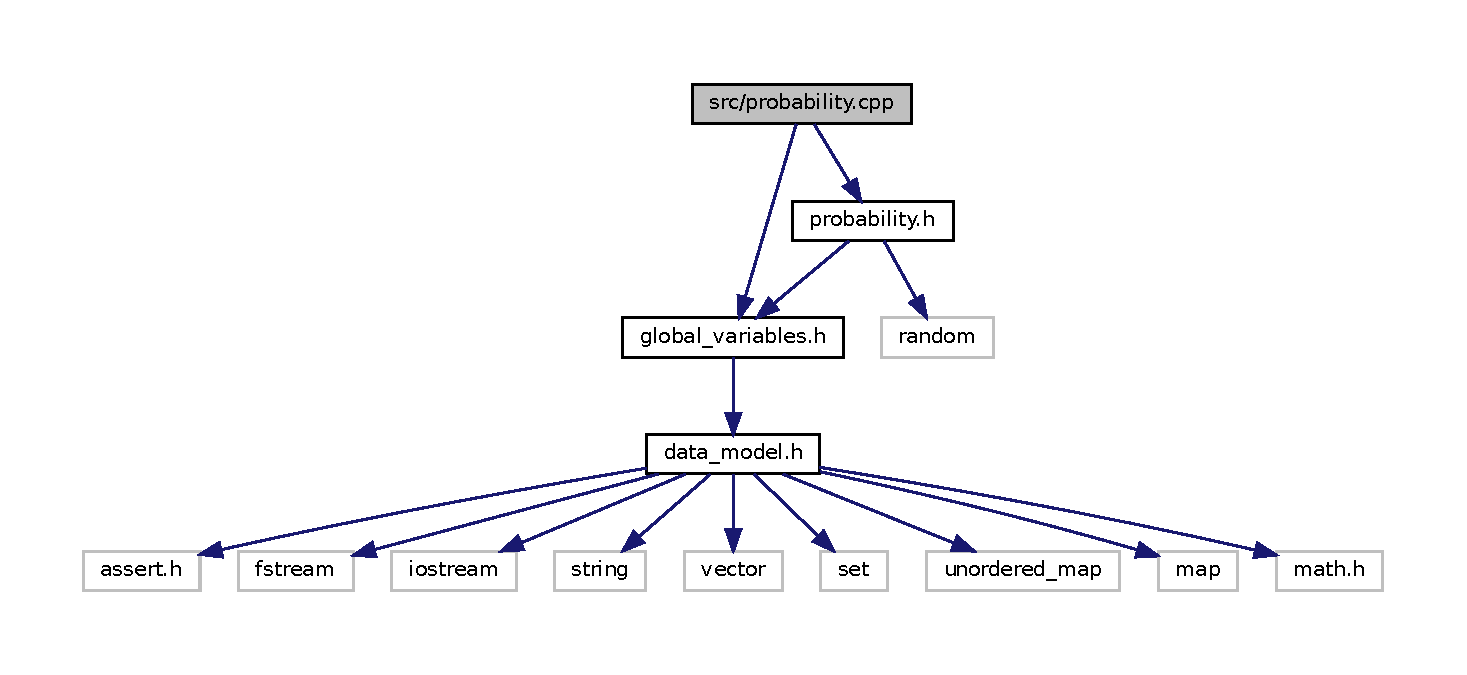
\includegraphics[width=350pt]{d1/d32/probability_8cpp__incl}
\end{center}
\end{figure}
\subsection*{Functions}
\begin{DoxyCompactItemize}
\item 
\mbox{\Hypertarget{probability_8cpp_a7e1fccef67213ff95a65f2a927e7c1c6}\label{probability_8cpp_a7e1fccef67213ff95a65f2a927e7c1c6}} 
uniform\+\_\+real\+\_\+distribution {\bfseries uniform} (0, 1)
\item 
\mbox{\Hypertarget{probability_8cpp_a6a1b9029d84d91d784ad861f0330fada}\label{probability_8cpp_a6a1b9029d84d91d784ad861f0330fada}} 
exponential\+\_\+distribution {\bfseries exponential} (1)
\item 
void \hyperlink{probability_8cpp_a59876affedc061069286bfd09a1c1d49}{init\+\_\+randomness} ()
\begin{DoxyCompactList}\small\item\em Initialize the pseudo-\/random number generator using specified seed. \end{DoxyCompactList}\end{DoxyCompactItemize}
\subsection*{Variables}
\begin{DoxyCompactItemize}
\item 
\mbox{\Hypertarget{probability_8cpp_a740e3e4f1bd0949f379c6ca7792d2fec}\label{probability_8cpp_a740e3e4f1bd0949f379c6ca7792d2fec}} 
random\+\_\+device {\bfseries ran\+\_\+dev}
\item 
\mbox{\Hypertarget{probability_8cpp_a29e835ad2ed1bccd97f457d7c0cb746e}\label{probability_8cpp_a29e835ad2ed1bccd97f457d7c0cb746e}} 
mt19937 \hyperlink{probability_8cpp_a29e835ad2ed1bccd97f457d7c0cb746e}{random\+\_\+variable}
\begin{DoxyCompactList}\small\item\em Our pseudo-\/random number generator. \end{DoxyCompactList}\end{DoxyCompactItemize}


\subsection{Detailed Description}
Additional functions dealing with probabilities. 



\subsection{Function Documentation}
\mbox{\Hypertarget{probability_8cpp_a59876affedc061069286bfd09a1c1d49}\label{probability_8cpp_a59876affedc061069286bfd09a1c1d49}} 
\index{probability.\+cpp@{probability.\+cpp}!init\+\_\+randomness@{init\+\_\+randomness}}
\index{init\+\_\+randomness@{init\+\_\+randomness}!probability.\+cpp@{probability.\+cpp}}
\subsubsection{\texorpdfstring{init\+\_\+randomness()}{init\_randomness()}}
{\footnotesize\ttfamily void init\+\_\+randomness (\begin{DoxyParamCaption}{ }\end{DoxyParamCaption})}



Initialize the pseudo-\/random number generator using specified seed. 

Uses a pseudo-\/random seed if seed == 0. 
\hypertarget{probability_8h}{}\section{src/probability.h File Reference}
\label{probability_8h}\index{src/probability.\+h@{src/probability.\+h}}


Inline functions dealing with probabilities.  


{\ttfamily \#include $<$random$>$}\newline
{\ttfamily \#include \char`\"{}global\+\_\+variables.\+h\char`\"{}}\newline
Include dependency graph for probability.\+h\+:\nopagebreak
\begin{figure}[H]
\begin{center}
\leavevmode
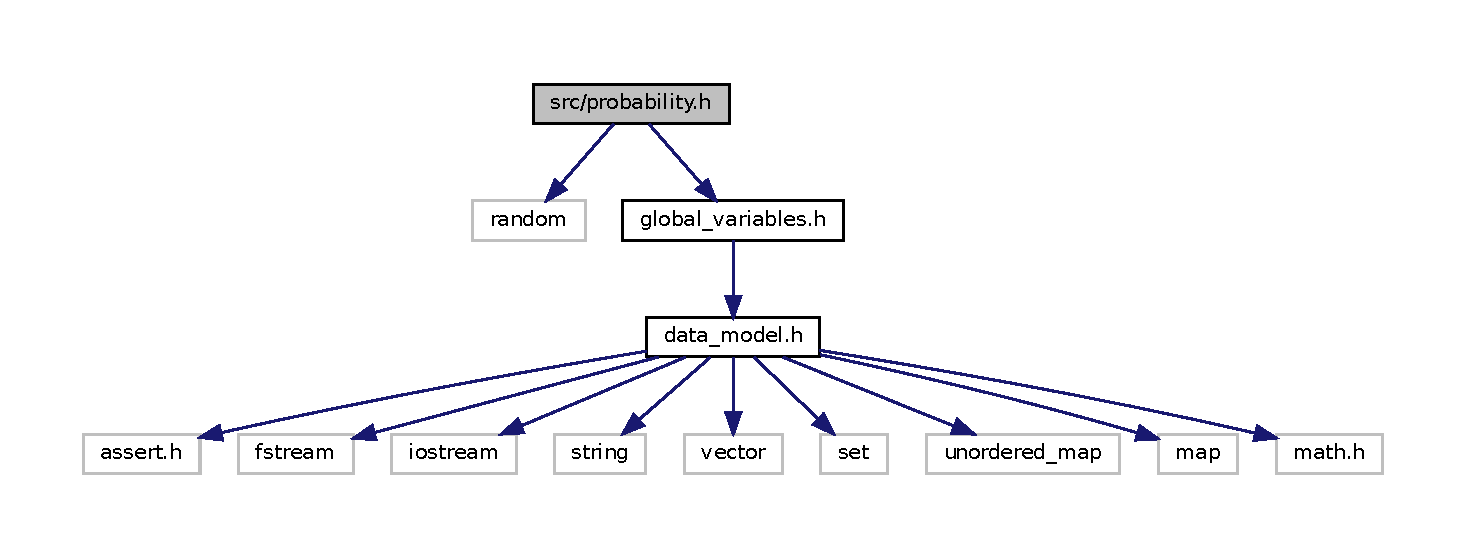
\includegraphics[width=350pt]{d6/dd3/probability_8h__incl}
\end{center}
\end{figure}
This graph shows which files directly or indirectly include this file\+:\nopagebreak
\begin{figure}[H]
\begin{center}
\leavevmode
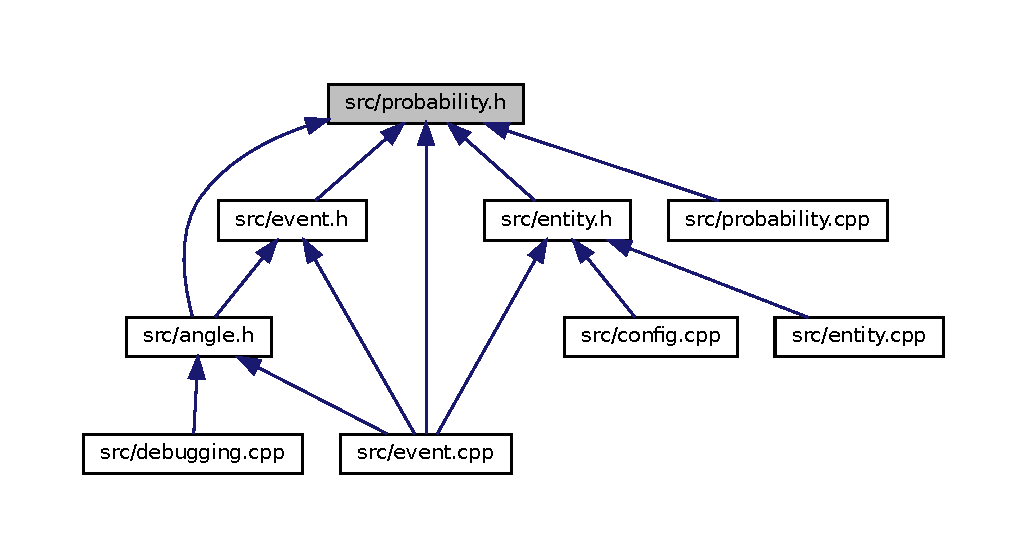
\includegraphics[width=350pt]{d4/de2/probability_8h__dep__incl}
\end{center}
\end{figure}
\subsection*{Functions}
\begin{DoxyCompactItemize}
\item 
void \hyperlink{probability_8h_a59876affedc061069286bfd09a1c1d49}{init\+\_\+randomness} ()
\begin{DoxyCompactList}\small\item\em Initialize the pseudo-\/random number generator using specified seed. \end{DoxyCompactList}\item 
double \hyperlink{probability_8h_a96d584ab7ce9c4874bd2a0305679755a}{tail2scale} (double tail)
\begin{DoxyCompactList}\small\item\em Compute the scale parameter for a tail index. \end{DoxyCompactList}\item 
\hyperlink{namespacetricl_af2e8973ba58a3dad9061296d8bee16a2}{probability} \hyperlink{probability_8h_a278b4df0353e94d6cf8cfb59a0d8058a}{probunits2probability} (\hyperlink{namespacetricl_af8f8f9076e92e1c664ffa96f18d038a5}{probunits} pu, double left\+\_\+tail, double right\+\_\+tail)
\begin{DoxyCompactList}\small\item\em Convert probability units to probability. \end{DoxyCompactList}\item 
\hyperlink{namespacetricl_ae42d2696f294300a43e0f5edf4875479}{rate} \hyperlink{probability_8h_abfaa763b93af36afec58f5d42fdf69a1}{effective\+\_\+rate} (\hyperlink{namespacetricl_ae42d2696f294300a43e0f5edf4875479}{rate} attempt\+\_\+rate, \hyperlink{namespacetricl_af8f8f9076e92e1c664ffa96f18d038a5}{probunits} success\+\_\+pus, double left\+\_\+tail, double right\+\_\+tail)
\begin{DoxyCompactList}\small\item\em Compute the current effective rate at which an event occurs from its current attempt rate and success probability units. \end{DoxyCompactList}\item 
\mbox{\Hypertarget{probability_8h_abd19a9ddc86a4f70890374440775af70}\label{probability_8h_abd19a9ddc86a4f70890374440775af70}} 
void \hyperlink{probability_8h_abd19a9ddc86a4f70890374440775af70}{add\+\_\+effective\+\_\+rate} (\hyperlink{namespacetricl_ae42d2696f294300a43e0f5edf4875479}{rate} er)
\begin{DoxyCompactList}\small\item\em Add effective rate to total, taking care of infinite values. \end{DoxyCompactList}\item 
\mbox{\Hypertarget{probability_8h_a0015fe9345db1abfdc66ca64cf7b28ff}\label{probability_8h_a0015fe9345db1abfdc66ca64cf7b28ff}} 
void \hyperlink{probability_8h_a0015fe9345db1abfdc66ca64cf7b28ff}{subtract\+\_\+effective\+\_\+rate} (\hyperlink{namespacetricl_ae42d2696f294300a43e0f5edf4875479}{rate} er)
\begin{DoxyCompactList}\small\item\em Subtract effective rate to total, taking care of infinite values. \end{DoxyCompactList}\item 
\hyperlink{namespacetricl_ae42d2696f294300a43e0f5edf4875479}{rate} \hyperlink{probability_8h_a597ea8b9a65b5faddf92c37de1a2c04f}{total\+\_\+effective\+\_\+rate} ()
\end{DoxyCompactItemize}
\subsection*{Variables}
\begin{DoxyCompactItemize}
\item 
\mbox{\Hypertarget{probability_8h_a29e835ad2ed1bccd97f457d7c0cb746e}\label{probability_8h_a29e835ad2ed1bccd97f457d7c0cb746e}} 
mt19937 \hyperlink{probability_8h_a29e835ad2ed1bccd97f457d7c0cb746e}{random\+\_\+variable}
\begin{DoxyCompactList}\small\item\em Our pseudo-\/random number generator. \end{DoxyCompactList}\item 
\mbox{\Hypertarget{probability_8h_a4719dce3f1f52de89aedc43c5149c801}\label{probability_8h_a4719dce3f1f52de89aedc43c5149c801}} 
uniform\+\_\+real\+\_\+distribution \hyperlink{probability_8h_a4719dce3f1f52de89aedc43c5149c801}{uniform}
\begin{DoxyCompactList}\small\item\em uniform(random\+\_\+variable) produces uniformly distributed numbers 0...1 \end{DoxyCompactList}\item 
\mbox{\Hypertarget{probability_8h_a00a3a3e47a0462049e9bc954f420b5e1}\label{probability_8h_a00a3a3e47a0462049e9bc954f420b5e1}} 
exponential\+\_\+distribution \hyperlink{probability_8h_a00a3a3e47a0462049e9bc954f420b5e1}{exponential}
\begin{DoxyCompactList}\small\item\em exponential(random\+\_\+variable) produces exponentially distributed numbers with mean 1 \end{DoxyCompactList}\item 
\mbox{\Hypertarget{probability_8h_a951c0f6989d7b3b3fd4361a7a1197149}\label{probability_8h_a951c0f6989d7b3b3fd4361a7a1197149}} 
const double \hyperlink{probability_8h_a951c0f6989d7b3b3fd4361a7a1197149}{scale0} = 1 / 2 / exp(1)
\begin{DoxyCompactList}\small\item\em Precomputed scale parameter for tail index 0. \end{DoxyCompactList}\end{DoxyCompactItemize}


\subsection{Detailed Description}
Inline functions dealing with probabilities. 



\subsection{Function Documentation}
\mbox{\Hypertarget{probability_8h_abfaa763b93af36afec58f5d42fdf69a1}\label{probability_8h_abfaa763b93af36afec58f5d42fdf69a1}} 
\index{probability.\+h@{probability.\+h}!effective\+\_\+rate@{effective\+\_\+rate}}
\index{effective\+\_\+rate@{effective\+\_\+rate}!probability.\+h@{probability.\+h}}
\subsubsection{\texorpdfstring{effective\+\_\+rate()}{effective\_rate()}}
{\footnotesize\ttfamily \hyperlink{namespacetricl_ae42d2696f294300a43e0f5edf4875479}{rate} effective\+\_\+rate (\begin{DoxyParamCaption}\item[{\hyperlink{namespacetricl_ae42d2696f294300a43e0f5edf4875479}{rate}}]{attempt\+\_\+rate,  }\item[{\hyperlink{namespacetricl_af8f8f9076e92e1c664ffa96f18d038a5}{probunits}}]{success\+\_\+pus,  }\item[{double}]{left\+\_\+tail,  }\item[{double}]{right\+\_\+tail }\end{DoxyParamCaption})\hspace{0.3cm}{\ttfamily [inline]}}



Compute the current effective rate at which an event occurs from its current attempt rate and success probability units. 

An effective rate of inf implies that the event occurs immediately.

\begin{DoxyReturn}{Returns}
the effective rate, 0...inf 
\end{DoxyReturn}

\begin{DoxyParams}[1]{Parameters}
\mbox{\tt in}  & {\em attempt\+\_\+rate} & the event\textquotesingle{}s current total attempt rate, 0...inf \\
\hline
\mbox{\tt in}  & {\em success\+\_\+pus} & the event\textquotesingle{}s current total success probability units, -\/inf...inf \\
\hline
\mbox{\tt in}  & {\em left\+\_\+tail} & the left tail index of the sigmoid function to be used, $>$= 0 \\
\hline
\mbox{\tt in}  & {\em right\+\_\+tail} & the right tail index of the sigmoid function to be used, $>$= 0 \\
\hline
\end{DoxyParams}
\mbox{\Hypertarget{probability_8h_a59876affedc061069286bfd09a1c1d49}\label{probability_8h_a59876affedc061069286bfd09a1c1d49}} 
\index{probability.\+h@{probability.\+h}!init\+\_\+randomness@{init\+\_\+randomness}}
\index{init\+\_\+randomness@{init\+\_\+randomness}!probability.\+h@{probability.\+h}}
\subsubsection{\texorpdfstring{init\+\_\+randomness()}{init\_randomness()}}
{\footnotesize\ttfamily void init\+\_\+randomness (\begin{DoxyParamCaption}{ }\end{DoxyParamCaption})}



Initialize the pseudo-\/random number generator using specified seed. 

Uses a pseudo-\/random seed if seed == 0. \mbox{\Hypertarget{probability_8h_a278b4df0353e94d6cf8cfb59a0d8058a}\label{probability_8h_a278b4df0353e94d6cf8cfb59a0d8058a}} 
\index{probability.\+h@{probability.\+h}!probunits2probability@{probunits2probability}}
\index{probunits2probability@{probunits2probability}!probability.\+h@{probability.\+h}}
\subsubsection{\texorpdfstring{probunits2probability()}{probunits2probability()}}
{\footnotesize\ttfamily \hyperlink{namespacetricl_af2e8973ba58a3dad9061296d8bee16a2}{probability} probunits2probability (\begin{DoxyParamCaption}\item[{\hyperlink{namespacetricl_af8f8f9076e92e1c664ffa96f18d038a5}{probunits}}]{pu,  }\item[{double}]{left\+\_\+tail,  }\item[{double}]{right\+\_\+tail }\end{DoxyParamCaption})\hspace{0.3cm}{\ttfamily [inline]}}



Convert probability units to probability. 

This is a smooth sigmoidal function that also depends smoothly on two tail indices as parameters. If both tail indices are zero, this is simply the expit (= inverse logit) function. If a tail index is positive, the corresponding tail converges with a power-\/law decay to its limit 0 (left tail) or 1 (right tail), where the power-\/law exponent is 1 / tail index.

\begin{DoxyReturn}{Returns}
the probability, 0...1 
\end{DoxyReturn}

\begin{DoxyParams}[1]{Parameters}
\mbox{\tt in}  & {\em pu} & the probability units, -\/inf...inf \\
\hline
\mbox{\tt in}  & {\em left\+\_\+tail} & the tail index of the left (lower) tail, $>$= 0 \\
\hline
\mbox{\tt in}  & {\em right\+\_\+tail} & the tail index of the right (upper) tail, $>$= 0 \\
\hline
\end{DoxyParams}
\mbox{\Hypertarget{probability_8h_a96d584ab7ce9c4874bd2a0305679755a}\label{probability_8h_a96d584ab7ce9c4874bd2a0305679755a}} 
\index{probability.\+h@{probability.\+h}!tail2scale@{tail2scale}}
\index{tail2scale@{tail2scale}!probability.\+h@{probability.\+h}}
\subsubsection{\texorpdfstring{tail2scale()}{tail2scale()}}
{\footnotesize\ttfamily double tail2scale (\begin{DoxyParamCaption}\item[{double}]{tail }\end{DoxyParamCaption})\hspace{0.3cm}{\ttfamily [inline]}}



Compute the scale parameter for a tail index. 

Auxiliary function for \hyperlink{probability_8h_a278b4df0353e94d6cf8cfb59a0d8058a}{probunits2probability()}.

\begin{DoxyReturn}{Returns}
the scale parameter, $>$ 0 
\end{DoxyReturn}

\begin{DoxyParams}[1]{Parameters}
\mbox{\tt in}  & {\em tail} & tail index to compute the scale parameter for, $>$= 0 \\
\hline
\end{DoxyParams}
\mbox{\Hypertarget{probability_8h_a597ea8b9a65b5faddf92c37de1a2c04f}\label{probability_8h_a597ea8b9a65b5faddf92c37de1a2c04f}} 
\index{probability.\+h@{probability.\+h}!total\+\_\+effective\+\_\+rate@{total\+\_\+effective\+\_\+rate}}
\index{total\+\_\+effective\+\_\+rate@{total\+\_\+effective\+\_\+rate}!probability.\+h@{probability.\+h}}
\subsubsection{\texorpdfstring{total\+\_\+effective\+\_\+rate()}{total\_effective\_rate()}}
{\footnotesize\ttfamily \hyperlink{namespacetricl_ae42d2696f294300a43e0f5edf4875479}{rate} total\+\_\+effective\+\_\+rate (\begin{DoxyParamCaption}{ }\end{DoxyParamCaption})\hspace{0.3cm}{\ttfamily [inline]}}

\begin{DoxyReturn}{Returns}
actual total effective rate, taking care of infinite values. 
\end{DoxyReturn}

\hypertarget{tricl_8cpp}{}\section{src/tricl.cpp File Reference}
\label{tricl_8cpp}\index{src/tricl.\+cpp@{src/tricl.\+cpp}}


Tri\+Cl, a generic model of social dynamics.  


{\ttfamily \#include $<$iostream$>$}\newline
{\ttfamily \#include \char`\"{}global\+\_\+variables.\+h\char`\"{}}\newline
{\ttfamily \#include \char`\"{}config.\+h\char`\"{}}\newline
{\ttfamily \#include \char`\"{}init.\+h\char`\"{}}\newline
{\ttfamily \#include \char`\"{}simulate.\+h\char`\"{}}\newline
{\ttfamily \#include \char`\"{}finish.\+h\char`\"{}}\newline
Include dependency graph for tricl.\+cpp\+:\nopagebreak
\begin{figure}[H]
\begin{center}
\leavevmode
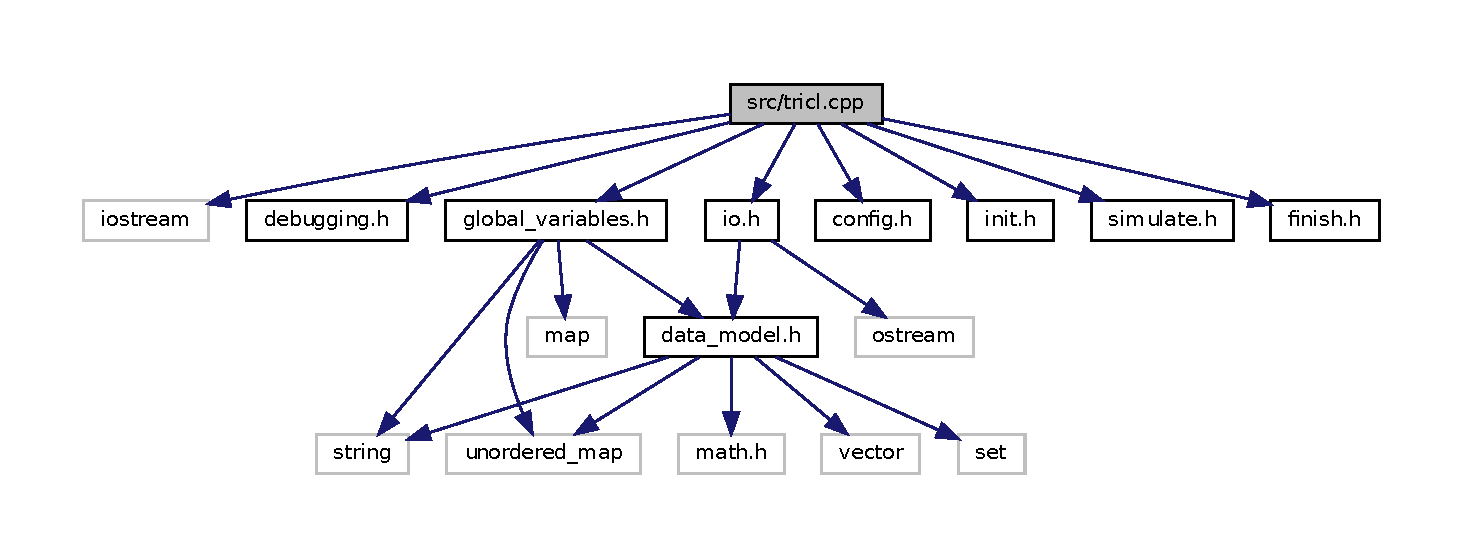
\includegraphics[width=350pt]{d0/d26/tricl_8cpp__incl}
\end{center}
\end{figure}
\subsection*{Functions}
\begin{DoxyCompactItemize}
\item 
\mbox{\Hypertarget{tricl_8cpp_ade42974a32e89c168c97127bbc971da4}\label{tricl_8cpp_ade42974a32e89c168c97127bbc971da4}} 
void \hyperlink{tricl_8cpp_ade42974a32e89c168c97127bbc971da4}{parse\+\_\+args} (int argc, const char $\ast$argv\mbox{[}$\,$\mbox{]})
\begin{DoxyCompactList}\small\item\em parse the command line arguments \end{DoxyCompactList}\item 
\mbox{\Hypertarget{tricl_8cpp_ac0f2228420376f4db7e1274f2b41667c}\label{tricl_8cpp_ac0f2228420376f4db7e1274f2b41667c}} 
int \hyperlink{tricl_8cpp_ac0f2228420376f4db7e1274f2b41667c}{main} (int argc, const char $\ast$argv\mbox{[}$\,$\mbox{]})
\begin{DoxyCompactList}\small\item\em main function of the tricl executable \end{DoxyCompactList}\end{DoxyCompactItemize}
\subsection*{Variables}
\begin{DoxyCompactItemize}
\item 
\mbox{\Hypertarget{tricl_8cpp_a6ff215d62218bc381c50ab2e7ef4731d}\label{tricl_8cpp_a6ff215d62218bc381c50ab2e7ef4731d}} 
string \hyperlink{tricl_8cpp_a6ff215d62218bc381c50ab2e7ef4731d}{config\+\_\+yaml\+\_\+filename}
\begin{DoxyCompactList}\small\item\em filename of configuration file \end{DoxyCompactList}\end{DoxyCompactItemize}


\subsection{Detailed Description}
Tri\+Cl, a generic model of social dynamics. 

\begin{DoxyAuthor}{Author}
Jobst Heitzig, Potsdam Institute for Climate Impact Research, \href{mailto:heitzig@pik-potsdam.de}{\tt heitzig@pik-\/potsdam.\+de} 
\end{DoxyAuthor}
\begin{DoxyDate}{Date}
Oct 18, 2019 
\end{DoxyDate}

%--- End generated contents ---

% Index
\backmatter
\newpage
\phantomsection
\clearemptydoublepage
\addcontentsline{toc}{chapter}{Index}
\printindex

\end{document}
